% Options for packages loaded elsewhere
\PassOptionsToPackage{unicode}{hyperref}
\PassOptionsToPackage{hyphens}{url}
\PassOptionsToPackage{dvipsnames,svgnames,x11names}{xcolor}
%
\documentclass[
  11pt,
]{book}
\usepackage{amsmath,amssymb}
\usepackage{lmodern}
\usepackage{iftex}
\ifPDFTeX
  \usepackage[T1]{fontenc}
  \usepackage[utf8]{inputenc}
  \usepackage{textcomp} % provide euro and other symbols
\else % if luatex or xetex
  \usepackage{unicode-math}
  \defaultfontfeatures{Scale=MatchLowercase}
  \defaultfontfeatures[\rmfamily]{Ligatures=TeX,Scale=1}
\fi
% Use upquote if available, for straight quotes in verbatim environments
\IfFileExists{upquote.sty}{\usepackage{upquote}}{}
\IfFileExists{microtype.sty}{% use microtype if available
  \usepackage[]{microtype}
  \UseMicrotypeSet[protrusion]{basicmath} % disable protrusion for tt fonts
}{}
\makeatletter
\@ifundefined{KOMAClassName}{% if non-KOMA class
  \IfFileExists{parskip.sty}{%
    \usepackage{parskip}
  }{% else
    \setlength{\parindent}{0pt}
    \setlength{\parskip}{6pt plus 2pt minus 1pt}}
}{% if KOMA class
  \KOMAoptions{parskip=half}}
\makeatother
\usepackage{xcolor}
\usepackage{longtable,booktabs,array}
\usepackage{calc} % for calculating minipage widths
% Correct order of tables after \paragraph or \subparagraph
\usepackage{etoolbox}
\makeatletter
\patchcmd\longtable{\par}{\if@noskipsec\mbox{}\fi\par}{}{}
\makeatother
% Allow footnotes in longtable head/foot
\IfFileExists{footnotehyper.sty}{\usepackage{footnotehyper}}{\usepackage{footnote}}
\makesavenoteenv{longtable}
\usepackage{graphicx}
\makeatletter
\def\maxwidth{\ifdim\Gin@nat@width>\linewidth\linewidth\else\Gin@nat@width\fi}
\def\maxheight{\ifdim\Gin@nat@height>\textheight\textheight\else\Gin@nat@height\fi}
\makeatother
% Scale images if necessary, so that they will not overflow the page
% margins by default, and it is still possible to overwrite the defaults
% using explicit options in \includegraphics[width, height, ...]{}
\setkeys{Gin}{width=\maxwidth,height=\maxheight,keepaspectratio}
% Set default figure placement to htbp
\makeatletter
\def\fps@figure{htbp}
\makeatother
\setlength{\emergencystretch}{3em} % prevent overfull lines
\providecommand{\tightlist}{%
  \setlength{\itemsep}{0pt}\setlength{\parskip}{0pt}}
\setcounter{secnumdepth}{5}
\usepackage{booktabs}
\usepackage{amsthm}
\usepackage{float}
\usepackage{fontspec}

%\setmainfont{cmunrm.otf}

\makeatletter
\def\thm@space@setup{%
  \thm@preskip=8pt plus 2pt minus 4pt
  \thm@postskip=\thm@preskip
}
\makeatother

\usepackage{a4wide}
\setlength{\parindent}{0in}
\setlength{\parskip}{1ex}
% grootte van de pagina


\setlength{\topmargin}{-0.25in}
\setlength{\oddsidemargin}{0.25in}
\setlength{\evensidemargin}{0.25in}
\setlength{\textwidth}{6.0in}
\setlength{\textheight}{9.0in}

\frontmatter
\pagenumbering{gobble}
\ifLuaTeX
  \usepackage{selnolig}  % disable illegal ligatures
\fi
\usepackage[]{natbib}
\bibliographystyle{apalike}
\IfFileExists{bookmark.sty}{\usepackage{bookmark}}{\usepackage{hyperref}}
\IfFileExists{xurl.sty}{\usepackage{xurl}}{} % add URL line breaks if available
\urlstyle{same} % disable monospaced font for URLs
\hypersetup{
  colorlinks=true,
  linkcolor={blue},
  filecolor={Maroon},
  citecolor={blue},
  urlcolor={blue},
  pdfcreator={LaTeX via pandoc}}

\title{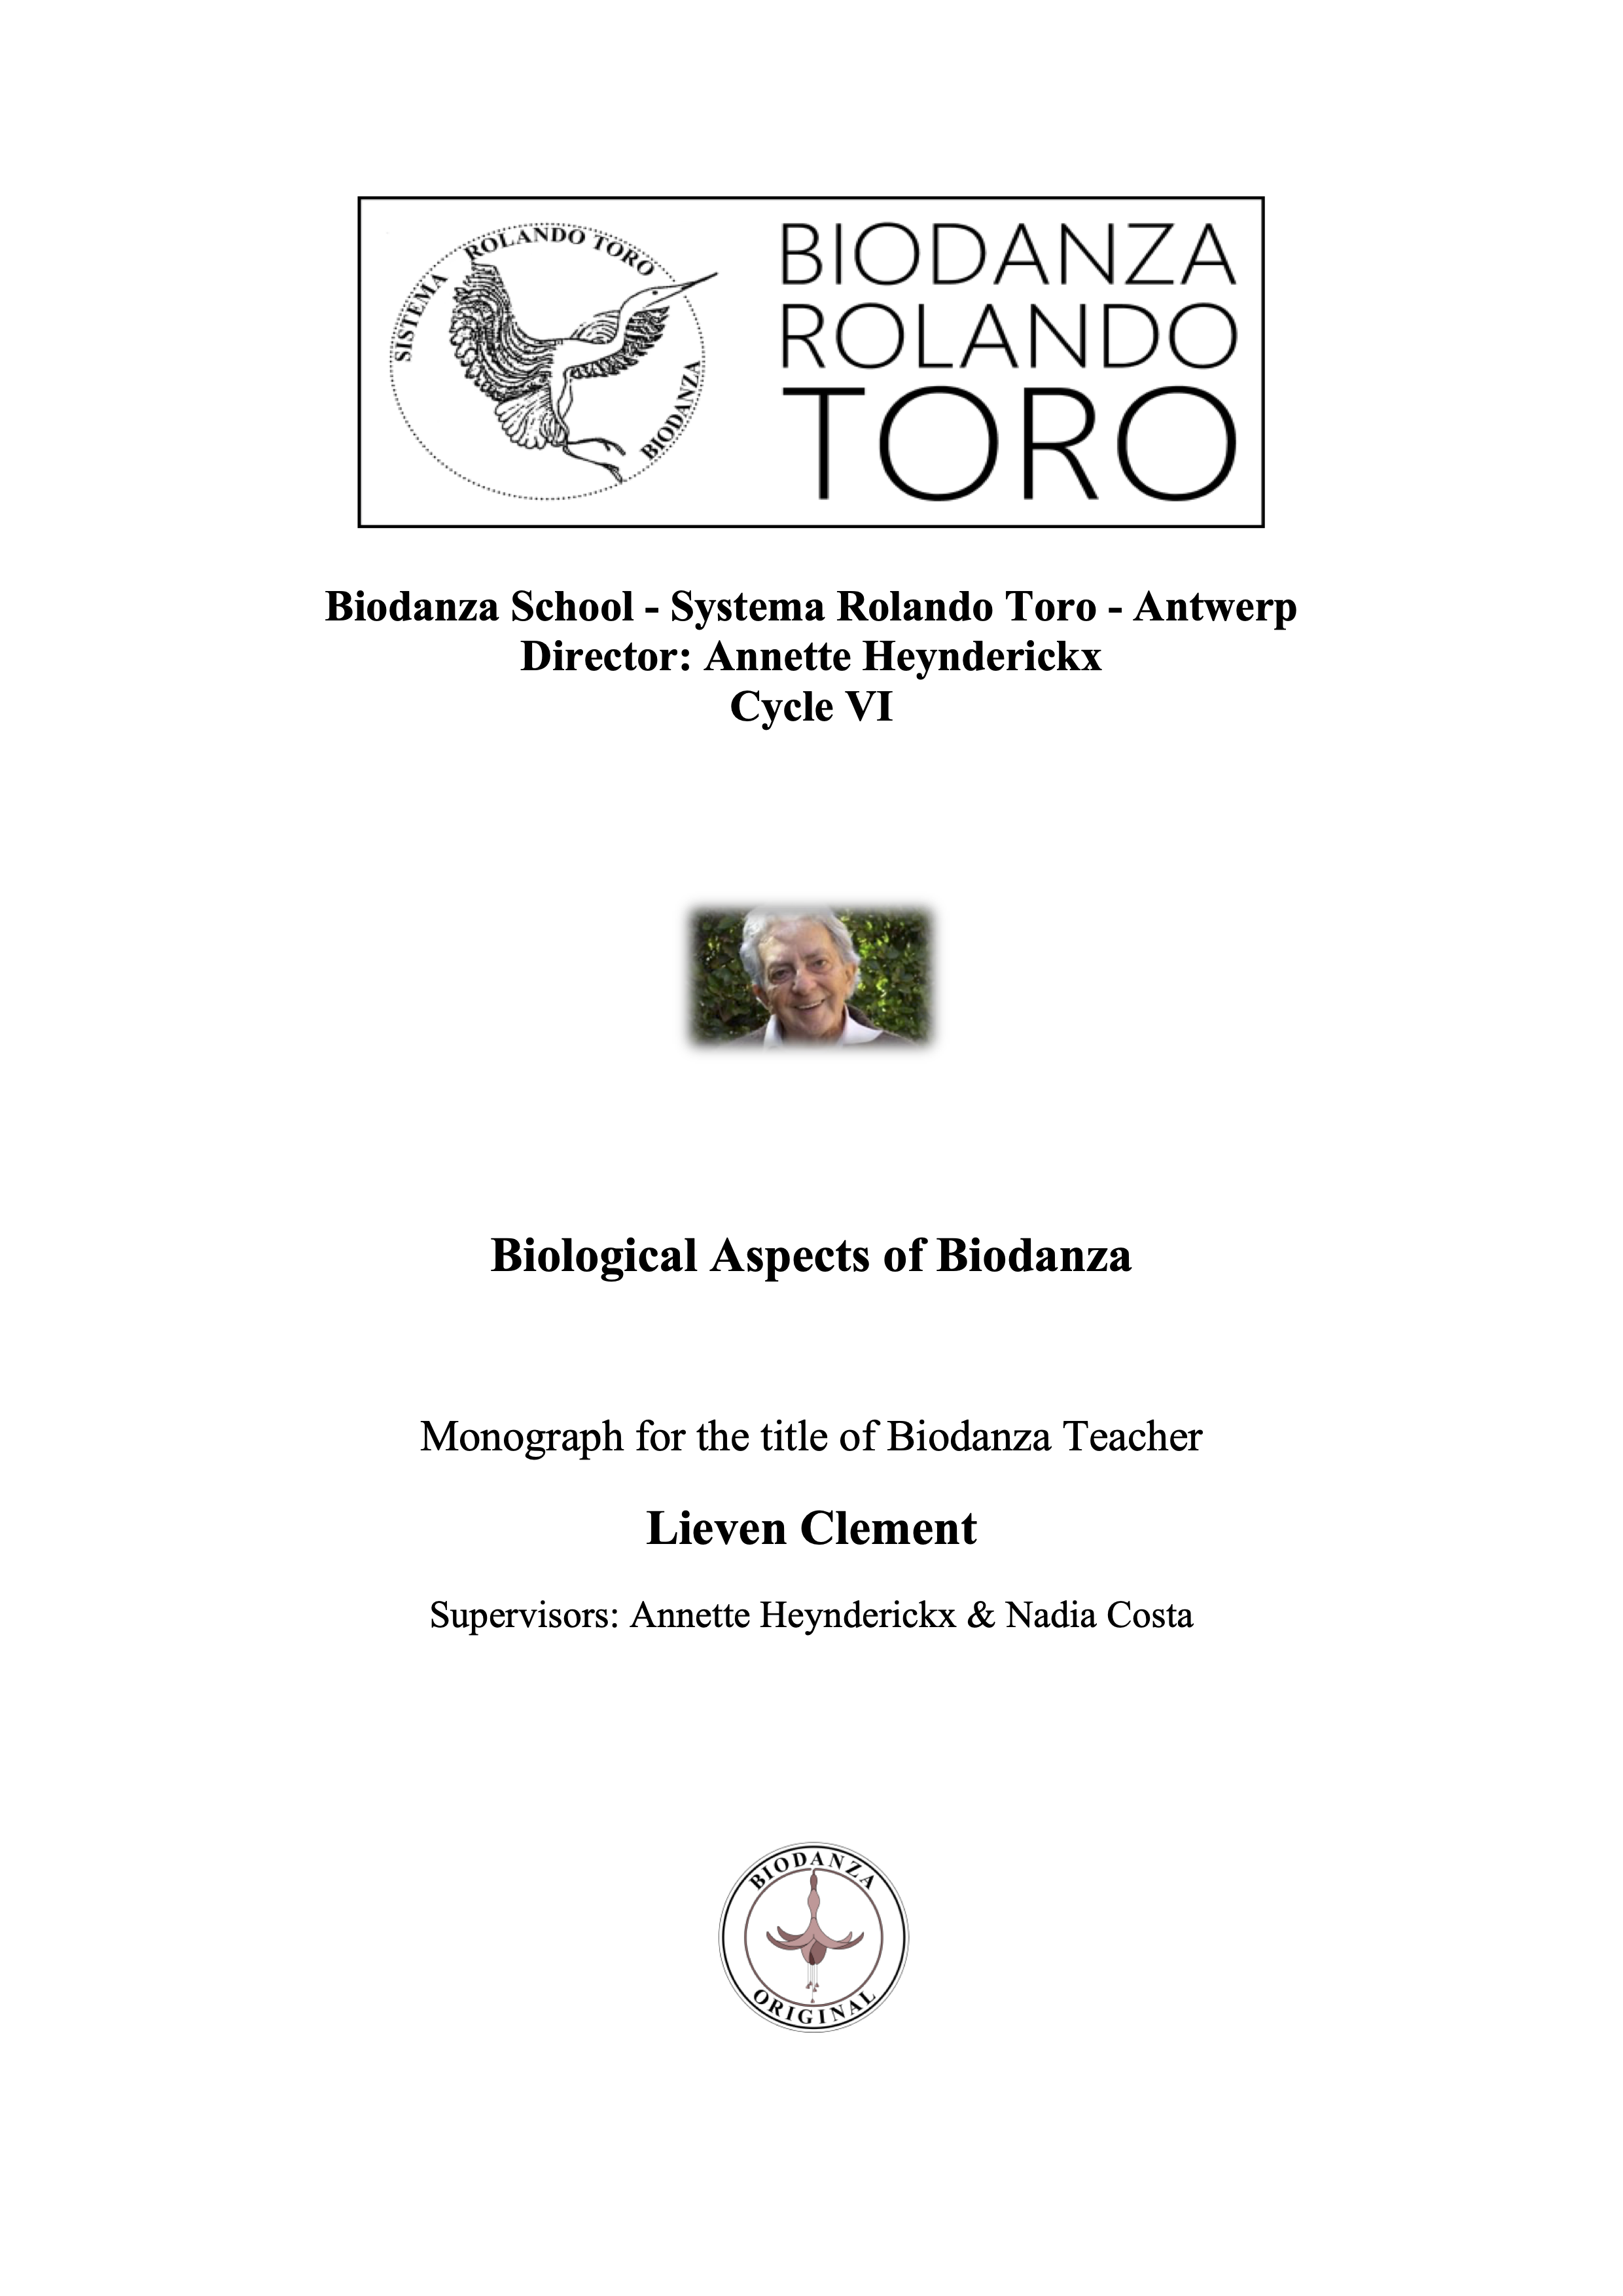
\includegraphics{figs/titlePage.png}}
\author{}
\date{\vspace{-2.5em}}

\begin{document}
\maketitle

{
\hypersetup{linkcolor=}
\setcounter{tocdepth}{2}
\tableofcontents
}
\hypertarget{section}{%
\chapter*{}\label{section}}
\addcontentsline{toc}{chapter}{}

\mainmatter

\hypertarget{licence-and-links}{%
\chapter*{Licence and links}\label{licence-and-links}}
\addcontentsline{toc}{chapter}{Licence and links}

This work is shared under the CC BY-NC-SA 4.0 licence on 22 August, 2023.

You may use the material for non-commercial purposes.

You are allowed to copy and redistribute the material in any medium or format and remix, transform, and build upon the material provided that you give proper credit to the author.

If you remix, transform, or build upon the material, you must distribute your contributions under the same license as the original.

A pdf version of this ebook can be found here: \href{https://biodanzabrugge.be/biologicalAspectsBiodanza/Biological-Aspects-of-Biodanza.pdf}{Biological-Aspects-of-Biodanza.pdf}

\hypertarget{summary}{%
\chapter*{Summary}\label{summary}}
\addcontentsline{toc}{chapter}{Summary}

I started the Biodanza teacher training in the School of Antwerp in 2021. Its enriched environment changed my views on life and how I experience life, entirely. It triggered a tremendous personal growth and stimulated me to reconnect my mind, body and hart.

From the first module of the teacher training, I was startled to see that the vertical axis in the model of Biodanza appeared to be so closely intertwined with my scientific path in the last 25 years. Indeed, Rolondo Toro had been inspired by so many leading scientists while developing his System of Biodanza. However, in my formal scientific education, I had never been exposed to many of the concepts that were touched upon in the first modules of the teacher training, and I could not comprehend these without consulting the work of the original authors.

My monograph, therefore, reflects my quest to understand Rolando's view on the biological aspects, which he enfolded in his model of Biodanza. In the first chapter, I introduce the model of Biodanza to put all readers on the same footprint. In the second chapter, I try to shed light on Rolando's view on life, his biocentric principle and vital unconsciousness. In this chapter I also lay the foundations for the remaining three chapters that each focus on an important biological aspect in the model of Biodanza: (1) Principles of cosmic life and the genesis of life, for which I give a short narrative on the history of the universe up to the origin of life, (2) Phylogenesis and evolution, in which I tells a brief story on the history of life and how life evolved, and, (3) Ontogenesis, where I shed some light on how we evolve from our origin as a fertilized egg cell up to our adult stage until we eventually die. In the latter chapter there is a strong focus on epigenetics, which is the missing link that Rolando Toro needed to explain how Biodanza can provide an enriched environment that induces change in how we use our genetic potential. Finally, I end this monograph with some concluding remarks and with an addendum with some additional texts and impressions that I have written during my Biodanza teacher training.

\hypertarget{intro}{%
\chapter{Introduction}\label{intro}}

My Biodanza journey started in 2018. Fien, my wife, took up the Biodanza teacher training and together we joined a weekly Biodanza group in Brugge. We quickly experienced the positive impact of our Biodanza practice on our lifes.

Two years later, true Biodanza magic happened.
In January 2019 my eldest son had a bike accident, which transformed our coupledom into a relationship of caring. In 2020, we realised that the events deepend our bound tremendously, however, at the cost of passion and attraction. Indeed, caring for each other implied us to alternate in strength to provide containment for the other, which drove us emotionally out of sync. Regardless of our efforts and mentally knowing what had to happen, it was difficult to get our feelings realigned.

Annette's Biodanza Summer Retreat in 2020 in the French Ardennes, was where the magic happened. The retreat started with an integrating vivencia (Biodanza session). The key exercise of the vivencia was the encounter. As soon as our eyes touched, I could see Fiens' emotions in her gaze and I knew that she felt the same. It happened in an instant, here and now, and ever since we have regained our emotional resonance. So this immense powerful vivencia did what all our mental work and struggle in 2020 could not accomplish.

How can Biodanza be so tranformative?
It uses the power of music and movement in an affective group to evoke vivencia, a deep experience with a strong bodily component. Vivencia happens here and now, and precedes our mental consciousness. It can triggers positive processes of change that continue well beyond Biodanza sessions and work through in our daily life.

\begin{figure}

{\centering 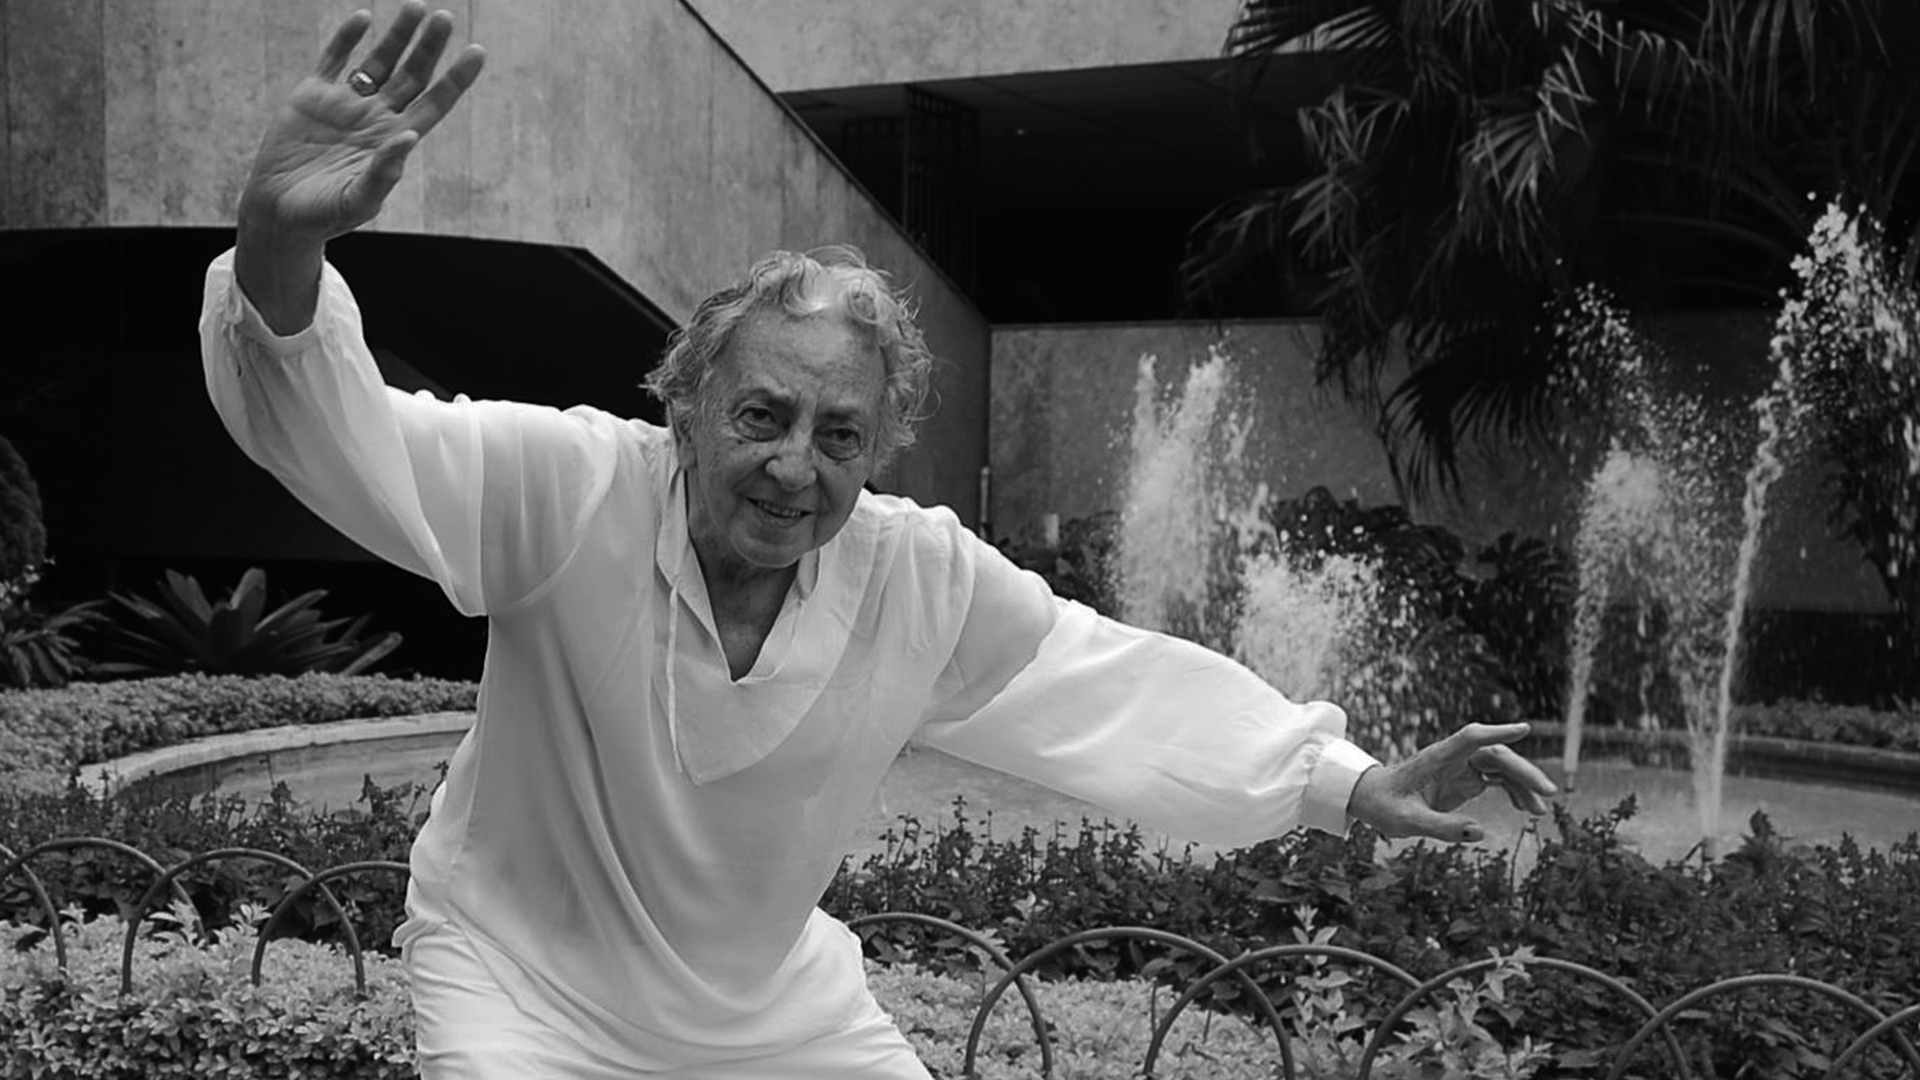
\includegraphics[width=0.45\linewidth]{./figs/rolando} 

}

\caption{Rolando Toro, the developer of Biodanza}\label{fig:rolandoToro}
\end{figure}

For Rolando Toro, the inventor and developer of Biodanza, the most important thing was: ``Vivencia, Vivencia, Vivencia''. Indeed, experiencing life through dance, music and movement enables us to deeply connect with our inner self, each other and the whole. Biodanza lets us feel that life is one and this through a deep and intense bodily experience.

With his system of Biodanza Rolando anticipated against the degeneration of humanity and the human society he observed during the second world war. For Rolando it was clear that modern human beings suffer from a disease he called ``society''. Our current society brings us far from our natural state of being, feeling, affection and sympathy, which can trigger anyone to extreme acts of violence and cruelty.

Therefore, he has developed his system of Biodanza from a nostalgia to love. A system that disseminates love and hope. A system that enables an affective re-education and that invites us to take part in a new way of live nourished by intense experiences.

Rolando was a passionate scientist and professor in psychology. He developed Biodanza from his own experiences and realized early on that his system has a strong foundation in the life sciences. During his development, he has also been inspired by the founders of modern dance and by primal people who still lay a deep meaning in each movement.

By rediscovering meaning in each of our movements, we ``re-humanize'' and can find how to truly live life deeply connected with the beauty of nature surrounding us.

\begin{figure}

{\centering 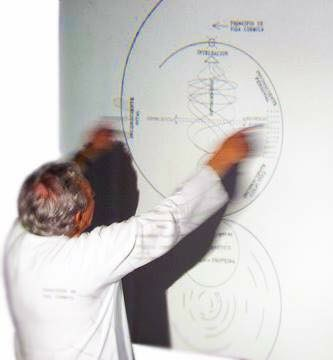
\includegraphics[width=0.45\linewidth]{./figs/rolandoAndModel} 

}

\caption{Rolando Toro explaining his Model of Biodanza}\label{fig:rolandoModel}
\end{figure}

Rolando has laid the foundation of his system during his career as a psychologist/researcher where he discovered the true impact of exercises that stimulate biological regression and identity, the first axis in his system. As opposed to the conventional mode of action in psychiatry, which has a starting point that is in essence symptomatic, for instance by dosing hormones or neurotransmitters that a patient is lacking, Rolando developed the vision that external stimuli (ecofactors) such as music, movement, touch, caressing, encounters and dance can induce us to reconnect to our self-healing potential. And this effectively stimulates us to tap into our genetic potential, which can promote immense growth and renewal both at a physiological and psycho-emotional level.

Growth and learning in Biodanza happens as how children learn: by seeing, imitating, experiencing and repetition, and, this deeply embedded in a enriched environment with positive reinforcement.

In this remainder of this chapter we will lay the foundation that is needed before delving into the biological aspects of Biodanza. We begin with the definition of Biodanza. We continue with the Biocentric Principle. We then introduce the model of Biodanza and we conclude with the aims of this monograph.

\hypertarget{definition-of-biodanza}{%
\section{Definition of Biodanza}\label{definition-of-biodanza}}

Rolando coined the term ``Biodanza'', which is a contraction of ``bios'', the Greek word for ``life'', and, ``danza'' the Italian word for dance. Here, the word ``danza'' is used in its original sense of ``natural movement'' that is full of meaning and well-connected with our emotions.

Rolando Toro defined Biodanza as a poetry of encounter. Indeed, all exercises can be seen as a preparation on the encounter with oneself, each other and the whole.

In Rolando's more academic definition Biodanza is a system of human integration, of organic renewal, of affective re-education and of re-learning the original functions of life.

The methodology of Biodanza consists of inducing integrating vivencia through music, movement and encounters in an affective group.

\hypertarget{vivencia}{%
\subsection{Vivencia}\label{vivencia}}

The concept of vivencia is key to understand the method of Biodanza.

Vivencia is an intense sensation of living, here and now, with a strong component of total organic sensation. It is a manifestation of being that precedes mental consciousness. Vivencia are passing experiences, e.g.~vivencia of fullness, of safety, of delight. The awareness of experiencing vivencia can come instantly or at a later moment and can give rise to deep emotions.

We do not have to try to rationalize our vivencia. They can been seen as manifestations of our bodily wisdom and spontaneously initiate integration and learning by experience. They are transformative experiences, which are the essence of the method of Biodanza. Indeed, our vivencia are key for growth and integration, and more important than mental consciousness. Nevertheless, practicing Biodanza might also induce a sense of awakening, but that is rather a side-product of noticing that actual growth has taken place upon embodying our vivencia.

\hypertarget{human-integration}{%
\subsection{Human Integration}\label{human-integration}}

Through vivencia a strong connection with life is established, which induces the integration with oneself, the human species and the universe.

The integration with oneself restores our psycho-physical unity, i.e.~the unity of the internal/psychic and external/physical world.

Integration with our fellow humans restores the connection within our species as a biological unity.

Integration with the universe re-unites us with nature and restores our intimate relation with the entire biosphere.
It lets us re-experience the deep connection of ourselves as part of the cosmos.

By restoring this connection to life, we can re-experience life to its very existence, here and now, which promotes growth and renewal on a biological, physiological and psycho-emotional level and can also be accompanied by a sense of a deep conscious awakening.

\hypertarget{organic-renewal}{%
\subsection{Organic Renewal}\label{organic-renewal}}

Biological systems possess the unique capacity of self-replication and self-organisation. However, stress, among others, can have a profound impact on cell and tissue maintenance and regeneration.

With transcendent Biodanza exercises we slow down our movements, lower our state of control and evoke a deep state of rest. This state is essential to switch on restoration and regeneration, and, reinforces homeostasis, i.e.~our bodies mechanism to maintain its equilibrium despite the changes in our environment.

\hypertarget{affective-re-education}{%
\subsection{Affective Re-education}\label{affective-re-education}}

In Biodanza many exercises stimulate and elicit affection and harmony, which can work through in our daily life by bringing harmony in our relation with ourselves, among each-other and with our environment.

\hypertarget{re-learning-of-the-original-functions-of-life}{%
\subsection{Re-learning of the Original Functions of Life}\label{re-learning-of-the-original-functions-of-life}}

Biodanza practice also reconnects us with our primal instincts, which are suppressed in our modern society and are often viewed as irrational behavior.
However, our instincts can be viewed as the biological wisdom of our species, which evolved for survival and maintenance of our species. By reconnecting ourselves with our innate impulses, we also restores harmony from within.

\hypertarget{sectionBiocentricPrinciple}{%
\section{Biocentric Principle}\label{sectionBiocentricPrinciple}}

The biocentric principle is at the heart of Rolando Torro's system of Biodanza. The biocentric principle considers the universe as the matrix of life, i.e.~a self-organizing structure that is building life. So not only living organisms, but, rather the entire cosmos is viewed as a massive living hologram.

This view invites people to radically rethink their relationship as a human being with the entire biosphere. Indeed, life itself becomes intrinsically sacred, which probes us to put all of life, and thus the entire universe, at the heart of our weltanschauung.

To me, it seems an invitation to gravitate from humanism, with human beings at its center, back to the view of primal cultures where the environment we are living in is not seen as the stage upon which we tread, but as an entity with whom we can communicate and build a deep intimate relationship.

Vivencia is the unique path to experience the Biocentric Principle and to genuinely become aware of it. This through our embodied mind, that also connects to that deeper knowledge that lies hidden in our inner self, ready to be touched by the intimate vivencial experience.

\hypertarget{sectionModelOfBiodanza}{%
\section{Model of Biodanza}\label{sectionModelOfBiodanza}}

Rolando Toro developed a scheme of his model of Biodanza that summarizes its foundation in the life sciences and its methodology, which is displayed in Figure \ref{fig:model}.

\begin{figure}

{\centering 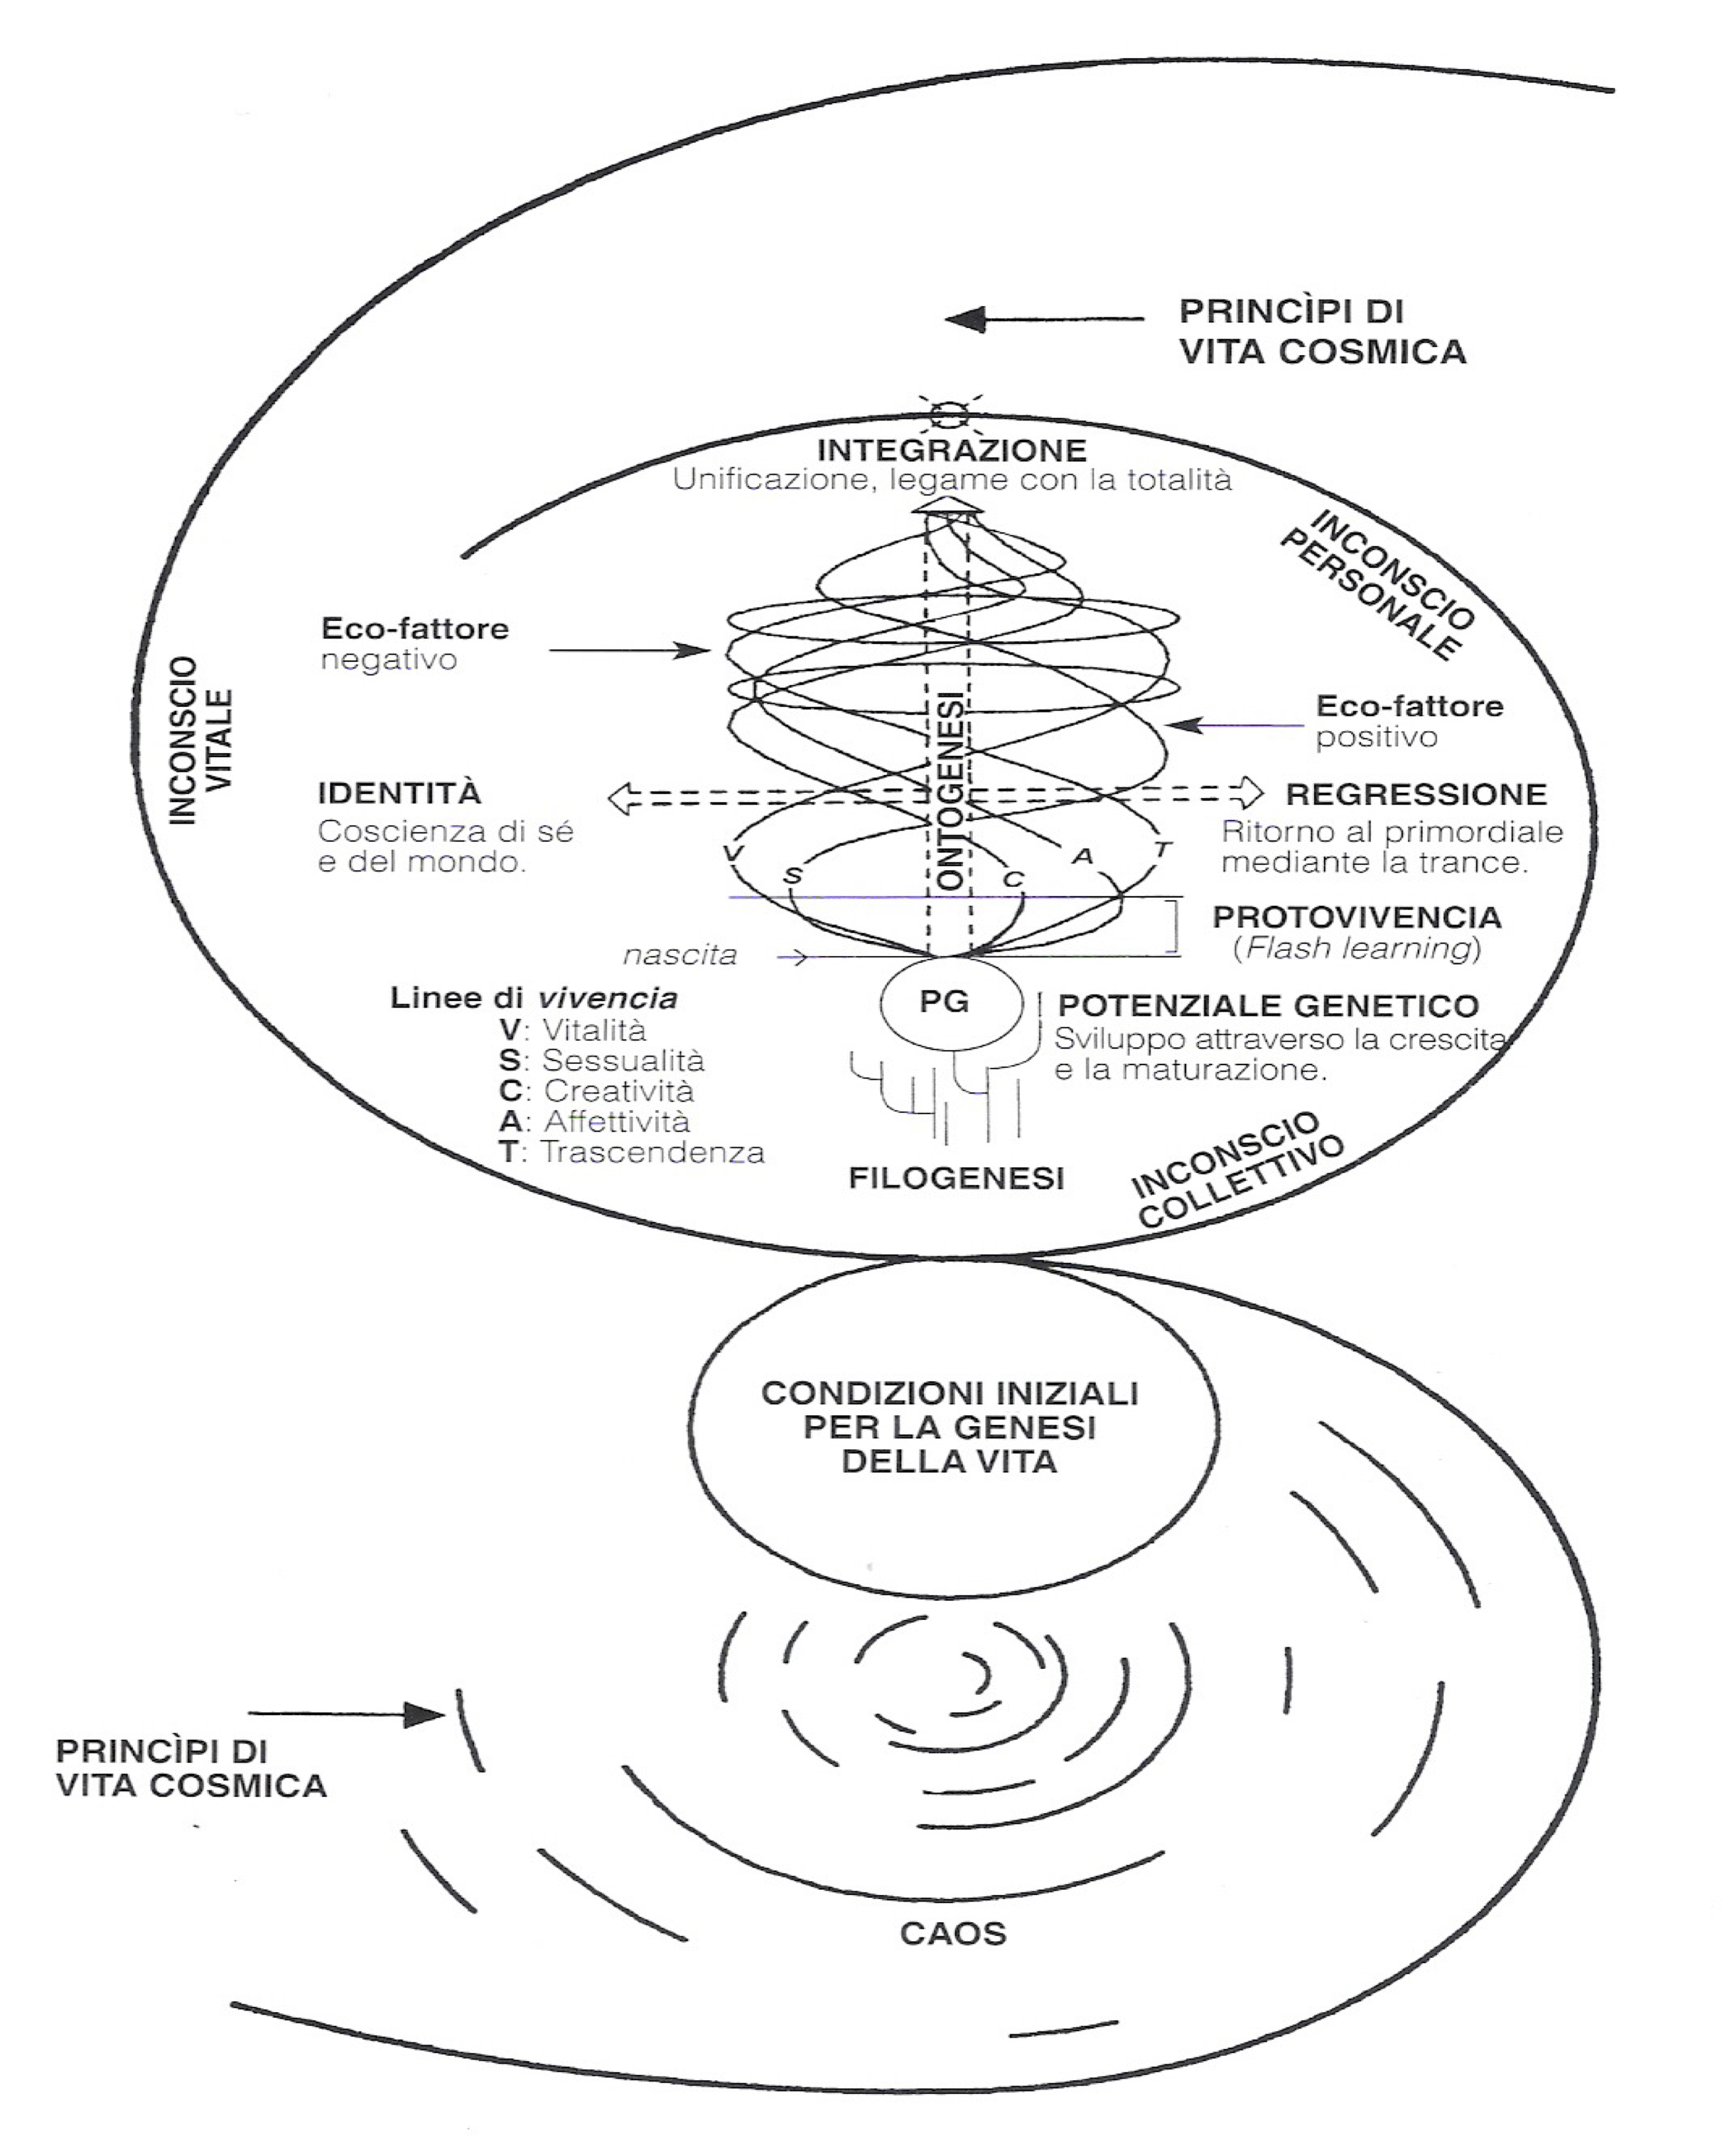
\includegraphics[width=1\linewidth]{./figs/biodanzaModel} 

}

\caption{Model of Biodanza}\label{fig:model}
\end{figure}

In this section I will briefly introduce the biological aspects in the model of Biodanza, which is the main theme of this monograph. Next, I will briefly touch upon the methodology of Biodanza.

\hypertarget{biological-aspects-of-biodanza}{%
\subsection{Biological Aspects of Biodanza}\label{biological-aspects-of-biodanza}}

In Figure \ref{fig:model} we see that the biological aspects of Biodanza are forming the vertical axis, the skeleton, of the Model of Biodanza. Note, however, that these concepts also have an important sociological, psychological, emotional and mystic dimension as a very substantial part of our human life takes place in the symbolic social domain.

The vertical axis consists of

\begin{enumerate}
\def\labelenumi{\arabic{enumi}.}
\tightlist
\item
  Principals of cosmic life and genesis of life
\item
  Evolution and phylogenesis
\item
  Genetic potential and ontogenesis
\end{enumerate}

Our cosmos as we know it originated out of chaos. It started with a very energy-rich state. It quickly cooled down enough for energy to be converted into mass - the majority in hydrogen and a fraction in more heavy helium nuclei. Due to the gravitational force, matter then started to cluster in nebula and eventually formed stars.

In the stars all elements have been formed by nuclear fusion and with each supernova, i.e.~an explosion of a star at the end of its life, these elements/atoms are projected into space.

In space these atoms further reacted and formed more complex molecules that eventually gave rise to precursors (``forerunners'') of the biological building blocks of life.

In a remote corner of our milky way, an average galaxy, on an average planet, Earth, there originated unique conditions that made the \emph{genesis of life} possible.
This was initiated by a chemical evolutionary process that gave rise to molecules with increasing complexity ultimately leading to chemistry that enabled self-replication and self-organisation and to the four essential bio-molecules of which all life is built:

\begin{itemize}
\tightlist
\item
  Lipids that enable the formation of membranes that are separating the inside of the cell from the outer world,
\item
  Carbohydrates or sugars that are used as energy sink/resource and as a backbone of many bio-molecules,
\item
  Proteins, the workhorses in our cells that facilitate the majority of chemical reactions in our cells, and
\item
  Nucleic acids, DNA and RNA, that are used to store and use our genome, i.e.~the set of genes, we inherited from our parents.
\end{itemize}

Once the first living cells emerged, they started to evolve and through evolution, they gave rise to all other living beings. This process is also referred to as phylogenesis.

We, humans, are a leaf on a small branch of the tree of life. Each of us with our own genetic potential. Through the course of our life, we develop from a fertilized egg cell to an embryo, a child, up to a full grown adult until we eventually die. During this process, which is also referred to as ontogenesis, the way how we use our genes is changed.

Indeed, at the conception we inherit the structure of our cells from our biological mothers' egg cell and our genome from our biological mother and father. At first this egg cell has access to all genes. But, as the cell divides into a clump of cells that starts to differentiate in different tissues, these more specialized cells have only access to a restricted set of genes that are essential for their function. This happens through small molecules that interact with our DNA and can switch genes on or off.
The study of how our development, behavior, and environment can cause changes that affect the way our genes are used, is also referred to as epigenetics.

Epigenetic changes are passed in cell division to the two new cells that are formed, which makes a liver cell to remain a liver cell and a brain cell to remain a brain cell upon cell division.

Also, external stimuli and eco-factors can induce epigenetic changes and thus how we use our genetic potential.\\

Note, that its broader definition ontogenesis not only looks at the biological development of the species, but also at the biological development of the individual which also implies an important social, psychological and emotional component.
Indeed, it was exactly in this larger field that Rolando was operating. A field that lies at the interface of the life sciences, anthropology, psychology, physiology, art and mysticism, and from which he developed his system for growth and integration of an individual towards a state which he referred to with his metaphor ``the cosmic human''.

\hypertarget{methodology-of-biodanza}{%
\subsection{Methodology of Biodanza}\label{methodology-of-biodanza}}

Vivencia is the cornerstone of the method of Biodanza. It reconnects us with the essence of life, which can work through both at the psycho-socio-emotional and the physiological level. Indeed, when we experience a deep vivencia, this is accompanied by intense bodily experiences. So, a Biodanza session might induce physiological changes, and can trigger the production of hormones, neurotransmitters and proteins, which originate from the expression of specific genes in our body and brain.

By integrating our vivencia and repeating exercises, Biodanza can promote human growth and evolution. Indeed, people who practice Biodanza for a longer period also experience that it can have a deep impact on their life and their social interactions. Note, that this can also go hand in hand with changes at a biological - physiological level. Indeed, ecofactors can induce epigenetic changes that activate or silence the expression of genes, and new neural connections can also emerge or can be promoted. So practicing Biodanza can affect the expression of our genetic potential.

The methodology of Biodanza is the central part in the model of Biodanza see Figure \ref{fig:model}, which I view as the body that is added to the skeleton of life.

\hypertarget{music-movement-and-vivencia}{%
\subsubsection{Music, Movement and Vivencia}\label{music-movement-and-vivencia}}

Vivencia is evoked by means of music, movement and encounters in an affective group.

Music is a universal language and is a very powerful source of transformation. In Biodanza it has an essential function of evoking vivencia. Hence, the pieces of music used in Biodanza are very carefully chosen upon studying their emotional content, evaluating the organic effects they promote, and the type of vivencia they evoke; before they were added to the Biodanza repertoire \citep{toro2008}.

Movement is another universal language that can be transformative, and, also plays a key function in evoking vivencia. Hence, movements are also very carefully chosen in Biodanza exercises. They stem from natural movements of human beings, gestures used in `socializing rituals', such as giving hands, embracing, caressing, etc.; and archetypical gestures, which we also find back in art of all human cultures and traditions. The movements can be executed by anyone. However, their sophistication comes from the meaning, emotion and feeling that is laid in it by the participant, which are of key importance for the depth of the vivencia \citep{toro2008}.

So music, movement and vivencia form a gestalt. A tiny change to one component can radically alter the vivencial experience that emerges.
With the delicate choice of the sequence of Biodanza exercises, the sequence of vivencia, an overarching vivencia unfolds for the entire session.

Biodanza cannot be practiced in isolation. The encounter with each other is an essential component of movement and for generating a field that accommodates integration of oneself, with our human species and the whole.

\hypertarget{horizontal-axis-identity-and-biological-regression}{%
\subsubsection{Horizontal Axis: Identity and Biological Regression}\label{horizontal-axis-identity-and-biological-regression}}

Rolando has laid the foundation of his system during his career as a psychologist/researcher where he discovered the true impact of exercises that stimulate identity and biological regression, the horizontal axis in his system.

A Biodanza session typically starts with vital rhythmic exercises that make participants aware of their body and their identity.
Then we make the bridge to more deepening exercises where we slow down our movements to lower our state of control. This can evoke a deep state of rest, dissolution of our ego, transcendence and integration. Indeed a state of biological regression that is harmonious and progressive, which reactivates important physiological patterns and brings us in contact with our origin and self-healing potential, among others. In Biodanza regression always refers to this important state of biological regression.

\hypertarget{vertical-axis-five-lines-of-biodanza}{%
\subsubsection{Vertical Axis: Five Lines of Biodanza}\label{vertical-axis-five-lines-of-biodanza}}

Rolando structured our genetic potential in five lines: Vitality, Sexuality, Creativity, Affectivity and Transcendence. They are his translation of the biological concept of genetic potential towards a broader biological and socio-psycho-emotional realm in which human growth and development takes place.
In a Biodanza session we typically work in two or more of these lines.

In the model the five lines are spiraling around the vertical axis of ontogenesis. Indeed, a Biodanza session provides the ecofactors that induce growth in these five lines and that can have long-lasting effects on a genomic, physiological and psycho-socio-emotional level.

We already get exposed to these five lines very early on in our lives, which Rolando referred to as protovivicencia. Indeed, protovivencia are the experiences of a newborn in response to internal and external stimuli, e.g.~through attention, food, love, care, caressing among others.

The protovivencia go hand in hand with flash learning, the very rapid learning that happens in the first six months of a newborn. These protovivencia can also be structured according to the five lines of Biodanza. As Rolando described in his book Biodanza \citep{toro2008}, the protovivencia of vitality stem from movement, action and rest; the protovivencia of sexuality is induced by contact and caresses; that of creativity by expression and curiosity; that of affectivity by nourishment and protection; and that of transcendence by the harmony a child experiences with their environment and surroundings.

During a Biodanza session we let (a subset of) the five lines pulsate by a sequence of exercises that first strengthen our identity and then induce biological regression.
Exercises that strengthen identity let practitioners become more aware of themselves, the world around them and how they stand in that world. Exercises that stimulate biological regression on the other hand stimulates the ego to dissolve and promote a connection with our different levels of unconsciousness.

\hypertarget{unconsciousness}{%
\subsubsection{Unconsciousness}\label{unconsciousness}}

In the periphery of methodology of Biodanza in the Model (Figure \ref{fig:model}), we find the personal unconsciousness, collective unconsciousness and vital unconsciousness.
Which is a resonance with ideas and information on ourselves, our primal instincts and archetypes, and the information that pulsates in the matrix of life, respectively.

Indeed, when a father caresses his baby, he connects with
his personal unconsciousness through the bound he experiences with his child, with the Demeter or mother archetype in his collective unconsciousness, and, with his vital unconsciousness through the physiological response he experiences through the proteins, hormones and neurotransmitters that are expressed in his cells.

So many of our actions are steered by our unconsciousness.
Through Biodanza exercises aiming for biological regression and transcendence we can deeply connect with these three types of unconsciousness.

When practicing Biodanza on a longer term we thus stimulate our genetic potential towards integration and connectedness with ourselves, our species and life as a whole, which Rolando referred to with the metaphor ``the cosmic human''.

\newpage

\hypertarget{aims-of-this-monograph}{%
\section{Aims of this monograph}\label{aims-of-this-monograph}}

This monograph focuses on the Biological aspects of Biodanza. It is my impression on ``Module III: Vital Unconsciousness and Biocentric Principle'' and ``Module IV: Biological Principles of Biodanza'' of the Biodanza teacher training that I followed in the School of Antwerp.

In particular, I will try to place all concepts that appear in the official learning material of these two modules in the context of the Model of Biodanza. It is my humble attempt to provide more insight in these biological aspects for Biodanza teachers and enthusiasts who want to dive deeper into the scientific background of the System of Biodanza.

This attempt consists of four parts:

\begin{enumerate}
\def\labelenumi{\arabic{enumi}.}
\item
  ``What is Life'', in which I lay a basic foundation and introduce important biological concepts that might provide a deeper insight in the concepts Biocentric Principle and Vital Unconciousness.
\item
  ``Principles of Cosmic Life and the Genesis of Life'', a short narrative on the history of the universe up to the origin of life.
\item
  ``Evolution and Phylogenesis'', which tells a brief story on the history of life and how life evolved.
\item
  ``Ontogenesis'', where I shed some light on how our cells evolve from our origin as a fertilized egg cell up to our adult stage until we eventually die.
\end{enumerate}

While the remainder of this monograph focuses on the Biological Aspects of Biodanza, it is important, however, to keep in mind that it is not my intention to reduce the Model of Biodanza to its biological aspects, only. Indeed, many of the concepts that we will touch upon from a biological perspective also have an important sociological, psychological, emotional and mystic dimension as a very substantial part of our human life takes place in the symbolic social domain.

\hypertarget{what-is-life}{%
\chapter{What is Life?}\label{what-is-life}}

One of the key drivers for Rolando Toro to develop his System of Biodanza was the disconnection he observed of men and women from the cosmic matrix, throughout our Western history, which has generated destructive cultural forms. This resulted from our Cartesian way of thinking, which caused a fragmented view of life. Indeed, it implied a division between body and mind, humanity and nature, living matter and non-living matter, and it considers the universe as being analyzable in separately existing parts that more or less interact as parts of a machine \citep{bohm1980}. This fragmented world view disconnected us from the universe that we inhabit and broke up our human society into distinct religious, political, economical and racial groups, among others leading to the exploitation of our natural resources, plants, animals and of fellow humans.

Ronando, therefore, has put his biocentric principle against this old world view. When formulating his principle, Rolando started from the axiom that ``life is the essential condition for the genesis of the universe''. In his book on Biodanza \citep{toro2008} he refers to the universe as a living hologram or the matrix of life, i.e.~a self-organising structure that is building life, and his view is that the entire cosmos has to be understood as a gigantic living system, by itself. This principle invites us to radically rethink our relationship as a human being with the entire biosphere that we inhabit. From this point of view, life itself is intrinsically sacred, which probes us to put all living beings, or all of life, at the heart of our weltanschauung.

From my scientific background the axiom that ``life is the essential condition for the genesis of the universe'' appeared rather radical. However, I immediately felt that Biocentrism ``an sich'', which starts from the deep astonishment that life, as we know it, simply exists, and puts it at the hearth of our weltanschauung was key for Rolando's system of Biodanza. Indeed, it starts from the simple fact that life exists, here and now, and that cognition and human growth originate through the vivencia of life. The latter can trigger us to think about our origin and our place in the universe, but more important than these thoughts is the experience, which promotes a deeper cognition from within, and this immediately with our embodied mind that is touched by vivencia.

With his axiom, however, Rolando went one step further. Indeed, in his book on Biodanza \citep{toro2008}, he explicitly mentions that ``The universe exists because life exists'', and not that ``Life exists because the universe exists'', which triggered me to try to grasp his views on the matter. I quickly learnt that Rolando's rationale is deeply rooted in the work of leading scientists. Indeed, Rolando often refers to Christian de Duve and his quotes ``Life is a cosmic imperative'' and ``Life is an obligatory manifestation of matter, written into the fabric of the universe'', Ilya Prigogine's ``dissipative structures'', ``dissipative zones'' and ``attractors'', and Maturana and Varella's ``autopoesis'' and ``autopoetic units'', among others. Many of these were concepts to which I had never been exposed in my formal scientific education and that I could not comprehend without consulting the work of the original authors.

When thinking about science, however, it is crucial, as \citet{bohm1980} nicely formulates, to acknowledge that scientific theories are not ``true knowledge'' corresponding to ``the reality as is'', but rather ever-changing insights that are giving shape and form to how we view and experience the world. This reflects my quest in this monograph: to shed light on Rolando's insights on biological aspects, which he enfolded in his model of Biodanza.

\hypertarget{rolando-toros-view-of-life-and-his-biocentric-principle}{%
\section{Rolando Toro's View of Life and his Biocentric Principle}\label{rolando-toros-view-of-life-and-his-biocentric-principle}}

In his book of Biodanza Rolando argues that the universe can be understood as a living system and that ``the realm of life embraces much more than the plants, the animals and man. Everything that exists, from neutrinos to quasars, from the fine stone to the most subtle thought, is a part of this prodigious living system'', which he often refers to as a gigantic living hologram.

\hypertarget{holographic-analogy-for-the-universe}{%
\subsection{Holographic analogy for the universe}\label{holographic-analogy-for-the-universe}}

Where did Rolando's holographic analogy for the universe come from?
The term ``hologram'' was coined for a photographic recording of a light field that originates by the interference\footnote{Interference: when two waves come together they result in a new wave that can have an amplitude that is higher or lower if the waves are in phase or out of phase respectively. Suppose that two identical waves interfere, when they are completely in phase their peaks and valleys are aligned and their interference will result in a new wave with a peak and valley that is twice as high and twice as deep as each of the original waves (constructive interference). When the waves are completely out of phase the peak of the first wave aligns with the valley of the second wave and vice versa so their resulting wave will be flat, i.e.~both waves cancel eachother out (destructive interference). Interference can be observed for all types of waves, e.g.~light, radio, acoustic, surface water, electric, matter and gravity waves among others.} of an incoming light beam with the light of this beam that has been scattered by illuminating an object.
From the recording a 3D image can than reconstructed e.g.~see figure \ref{fig:hologram1}. The recording at every spot on the photographic plate is the result of the interference of light waves that are scattered by all locations of the object. Each part of the record thus contains information of the whole object unlike a traditional photograph where there is a point-to-point correspondence of the object and the recorded image. As \citet{bohm1980} nicely phrases it ``form and structure of the entire object may be said to be enfolded within each region of the photographic record'' and ``when one shines light on any region, this form and structure are unfolded to give a recognizable image of the whole object once again''.

\begin{figure}

{\centering 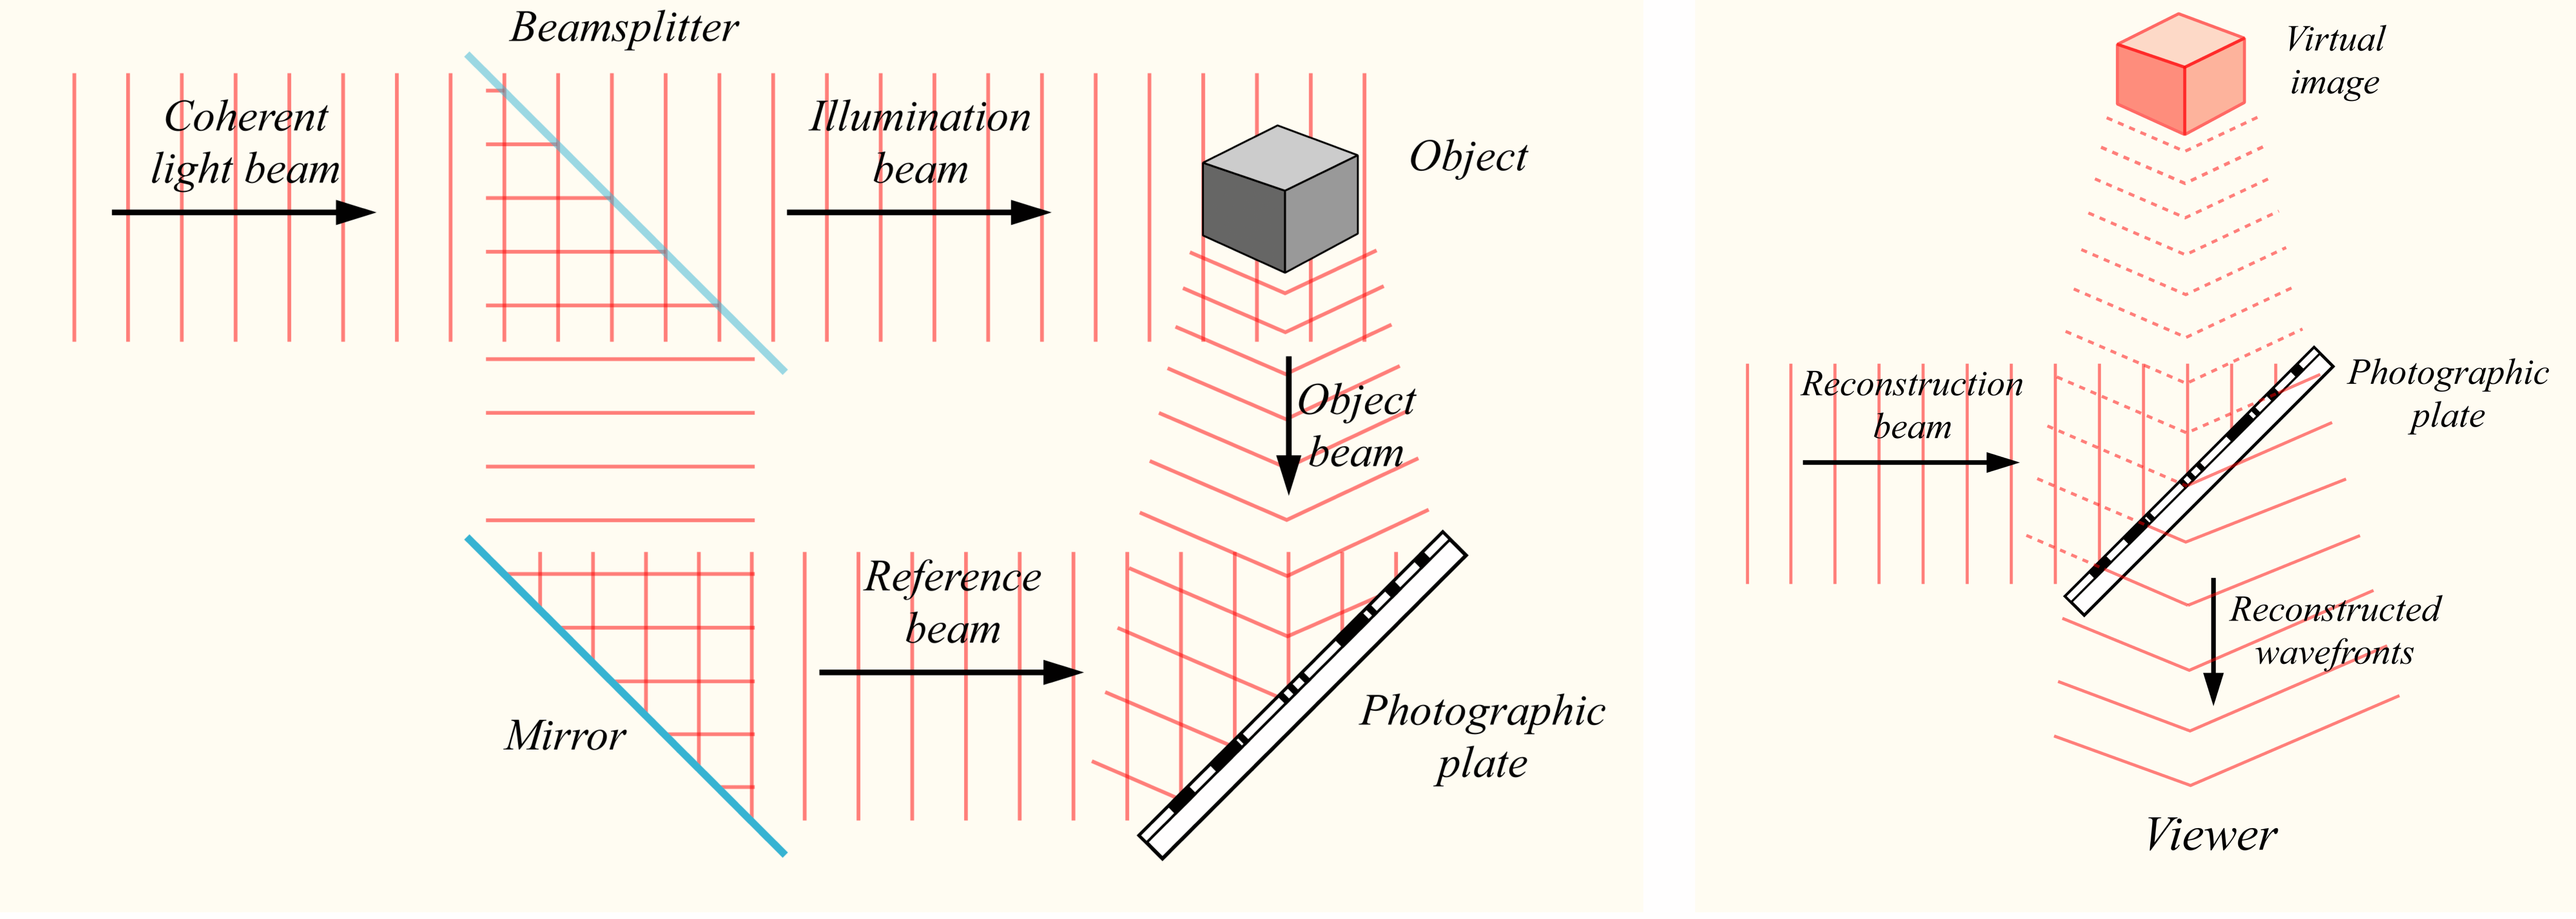
\includegraphics[width=1\linewidth]{./figs/holographySmall} 

}

\caption{Holographic recording and reconstruction. (Source: Bob Mellish, Wikipedia)}\label{fig:hologram1}
\end{figure}

In quantum mechanics, both matter and electromagnetic waves (such as light, microwaves and X-rays amongst others) have a particle and wave character, and every physical structure is defined by a wave function that in principle extends over the whole universe. As \citet{bohm1980} points out in an insightful example: ``when we look to the night sky we are able to discern structures covering immense stretches of space and time, which are in some sense contained in the movements of light in the tiny space encompassed by the eye and (\ldots) also how instruments (\ldots) can discern more and more of this totality, contained in each region of space.'' This illustrates how according to these insights, information on the entire universe, or on its \emph{total order}, is \emph{enfolded} or contained in some implicit sense, in every region of space-time and how it can be \emph{unfolded} by our eye or instruments. \citet{bohm1980} further argues that this enfoldment and unfoldment does not only applies to light waves, but extends to electromagnetic waves in general, as well as to other waves such as to the electronic, protonic, gravitational, sound waves, etc. and even towards fields that are yet unknown and may be discovered later.

\citet{bohm1980} therefore replaced the old Cartesian analogy of the universe as a machine by a novel analogy: that of a holographic universe, which refers to its unbroken and undivided totality that is enfolded in every region of space-time.

So when Rolando was referring to the universe as a living hologram, he expressed his view that life is part of this unbroken and undivided totality that is enfolded in every region of space-time.

To get a better understanding of this view, we will introduce Bohm's example of a seed from which an entire plant is growing. The plant is also holographic. Indeed each of its cells contains all information from the seed, i.e.~all its DNA as well as its cellular structure. \citet{bohm1980} further points out that the seed contains little to nothing from the actual biomass of the plant that it has developed. The seed merely contains the information that is required to transform its environment to grow the plant from solar energy and the chaos of simple molecules CO\(_2\), nitrogen, phosphorous, etc. Remarkably, the plant will eventually produce new seeds, which will spread its information further throughout the environment and will transform it over and over again to grow plants. It thus becomes obvious that we no longer need to make the distinction between ``inanimated'' and ``animated'' matter. Indeed, if we would stick to this old Cartesian way of thinking we are confronted with confusing questions like when would a so-called ``inanimated'' carbon atom become animated? As soon as it enters the leaf stomata or when it transformed into an organic compound? Does the carbon atom becomes inanimated again when it is released from the plant as it burns the sugars it has assimilated into CO\(_2\) during the night? All these confusing questions spontaneously resolve when considering the universe as an unbroken and undivided totality. Indeed, from this paradigm we consider that the environment is augmented with the information of the seed, which somehow seems to direct its environment to grow a corresponding plant. So life itself can be regarded as belonging to a totality including plant and the environment. Life is somehow enfolded in this totality and already implicitly present even before it is unfolded and explicitly manifests itself. Indeed, the ensemble of all atoms that eventually will form the plant that will grow from a certain seed are already present in the environment. In this way, so-called ``inanimated matter'' can be seen as a subtotality of the whole in which life can be unfolded, for instance when the environment is enriched with the information from a plant seed. So \citet{bohm1980} concludes that ``we do not need to fragment the whole into life and inanimated matter, nor do we have to try to reduce life completely to nothing but an outcome of the latter''.

\hypertarget{the-universe-as-a-self-organising-structure}{%
\subsection{The universe as a self-organising structure}\label{the-universe-as-a-self-organising-structure}}

Rolando also referred to the universe as a self-organising structure that is building life. The universe as we know it likely started off with the big bang: a massive spike of energy. Shortly after the big bang, matter was formed. As \citet{davies1987} describes it, this matter was rather formless existing of subatomic particles more or less uniformly distributed in space at a more or less uniform temperature.
Paul Davies further argues that the universe than gradually has been unfolding from this largely featureless state towards its current richness in physical and chemical forms and structures as it is ageing. Or to quote him: ``the creative power of nature manifested mainly AFTER the initial flash of existence''. Indeed, the creative ability of nature continues through all time.

Ilya Prigogine was one of the first scientists who developed the theory to explain how matter and energy have the innate ability to bring about self-organising processes. Convection currents are for instance an example of a simple physical process generating massive structures. They can be observed when simply heating a shallow layer of fluid or gas from below, which establishes a temperature gradient that lets the fluids rest state to become unstable. Indeed, the warmer fluid at the bottom is lighter and starts to float to the top where it cools down again, whereas the colder fluid at the top is more heavy and sinks to the bottom, where it is heated. Large ensembles of molecules therefore start to exhibit coherent patterns of motion (see Figure \ref{fig:convectionCells}).

\begin{figure}

{\centering 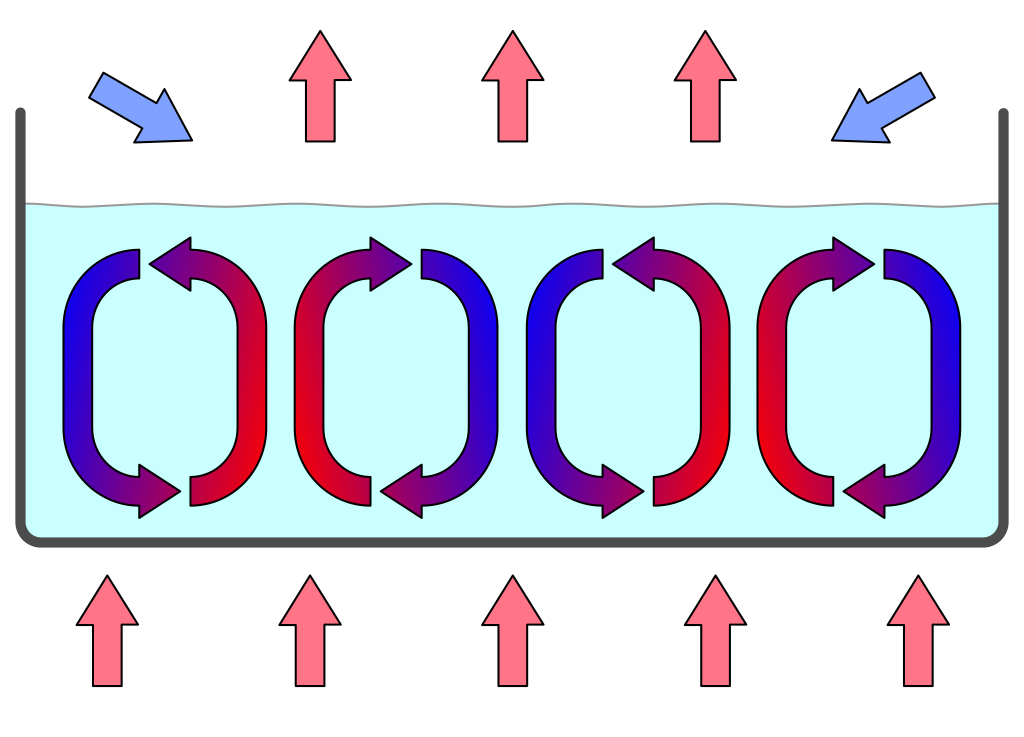
\includegraphics[width=0.8\linewidth]{./figs/convection_cells} 

}

\caption{Convection cells in a gravitational field. A fluid layer is heated from the bottom. The warmer fluid at the bottom becomes lighter and floats to the top where it cools down again, whereas the more heavy colder liquid sinks to the bottom where it is heated. This organizes the fluid layer in hexagonal convection cells (Source: Wikipedia - users Eyrian and Con-struct)}\label{fig:convectionCells}
\end{figure}

The convection motion leads to a spontaneous complex spatial organisation, almost a dance, of billions of molecules moving coherently and forming hexagonal convection cells. Such convection cells can be observed in a small dish of a fluid in a lab, up to the level of the earth's atmosphere and the solar photosphere (see movie below).

\emph{Movie of the solar photosphere observed with the Swedish 1-m Solar Telescope (SST) on La Palma, Spain. The movie shows solar granulation which is a result of convective motions of bubbles of hot gas that rise from the solar interior. When these bubbles reach the surface, the gas cools and flows down again in the darker lanes between the bright cells. In these so-called intergranular lanes, we can also see small bright points and more extended bright elongated structures. These are regions with strong magnetic fields. (Source: Wikipedia, user Luc.rouppe, link: \url{https://en.wikipedia.org/wiki/File:Granulation_Quiet_Sun_SST_25May2017.webm})}

Prigogine showed that spontaneous self-organisation also occurs in chemical systems that are operated far from equilibrium by continuously pushing matter and energy through it. These self-organising processes are largely unpredictable and spontaneously arise in our universe.
\citet{prigogineStengers1984} further argue that such chemical and physical processes are the basis of the complex self-organisation that we observe in living systems.

So instead of clinging to the destructive division of humanity and nature, or to the equally destructive idea that we humans are an incidental and irrelevant feature of the cosmos, we rather can embrace ourselves as children of our universe. A result of its remarkable creativity with a beauty similar to all magnificent self-organising structures that are surrounding us.

\hypertarget{organisation-of-this-chapter}{%
\subsection{Organisation of this chapter}\label{organisation-of-this-chapter}}

The remaining of this chapter builds on the work of five scientists who were very influential and whose insights can help us to increase our understanding on the biological aspects that Rolando Toro included in his Model for Biodanza:

\begin{itemize}
\tightlist
\item
  Erwin Schrödinger who explicitly defined life as structuring ``order-from-disorder'',
\item
  Ilia Prigogine who developed the theory for this and coined the term ``Dissipative Structures'',
\item
  Christian de Duve one of the founding fathers of biochemistry, and
\item
  Humberto Maturana and Francisco Varela with their concept of autopoiesis.
\end{itemize}

Note, that the subsections in ``Christian de Duve: a biochemical view of life'' always start with a general overview followed with subsections including more technical details. I have chosen to include these technical details in this monograph because they can help interested readers to understand all terms and concepts that are only touch upon very briefly in the reader of the Biodanza teacher training ``Module IV: Biological Principles of Biodanza''. The sections ``Maturana and Varela: a Systems View of Life'' and ``Links to Vital Unconsciousness'' are more philosophical in nature.

\hypertarget{schruxf6dinger-and-prigogine-a-thermodynamic-view-of-life}{%
\section{Schrödinger and Prigogine: a Thermodynamic View of Life}\label{schruxf6dinger-and-prigogine-a-thermodynamic-view-of-life}}

In his seminal lecture series: ``What Is Life? The Physical Aspect of the Living Cell'' \citet{schrodinger1944} defined life as

\begin{enumerate}
\def\labelenumi{\arabic{enumi}.}
\item
  an open system that can generate order from chaos by exploiting external energy sources,
\item
  with the capacity to transmit its own specific blueprint from generation to generation.
\end{enumerate}

Note, that in his seminal lecture series \citet{schrodinger1944} also laid out key functions of the molecule that was involved in this specific blueprint and this while DNA was not even discovered.

At first, the property that life can generate order or structure seems to contradict the second law of thermodynamics that states that: a system is always gearing towards maximal entropy.

Entropy can be loosely defined as a physical quantity for the level of how energy is spread out. It is thus the tendency of a system to evolve from a concentrated energy state to an energy state that is more spread out. This can be easily understood from a simple example known to each of us: if you put a hot pot in a large room, the pot will cool down and the temperature in the room will slightly rise until the pot and the room have the same temperature. As a result the concentrated heat energy from the pot is nicely spread out over the entire room.

Schrödinger understood that life was not violating this second law. Indeed, by being an \emph{open} system, it can interact with the environment, and by eating and breathing there has to be a way of ``concentrating order'' or maintaining a higher more concentrated energy state.

Prigogine was the first one who provided the theoretical framework for a type of chemistry that is key for life \citep{prigogineStengers1984}. He realized that the chemistry of life is totally different from most chemical systems that were studied up to then. Indeed, the chemistry and processes of life are highly non-linear with many feedback loops\footnote{A feedback loop in a chemical system occurs if part of the produced molecules are used again as input} and are operated far from equilibrium by continuously pushing matter and energy through it.

We intuitively know the latter: our body is typically at a higher energy state than the corresponding material in a non-living state. We can simply acknowledge that as we are hotter than the room, and a crude way to estimate how long we are death is by measuring the temperature of a corpse. To maintain our higher energy state, to concentrate chemicals in our cells, and, to build complex molecules, cells and tissues from it, we have to keep on eating and breathing.

\hypertarget{dissipative-structures}{%
\subsection{Dissipative structures}\label{dissipative-structures}}

Prigogine discovered that complex self-organising systems can spontaneously arise if they are open and can exchange lots of energy and matter with their surroundings.
Key for it is a chaos of matter and a flow of energy through the system.
In chemical systems, and life is to a large extent chemistry, the influx of energy allows the generation of structure while producing lots of entropy by dissipation. Dissipation means that energy has been converted from one energy form to another and that it can no longer be converted back in its original form. So dissipation is irreversible, which adds the arrow of time to life. Indeed conversion of energy to heat inherently takes place in all underlying chemical reactions and these cannot be reversed without the addition of new energy. Hence, a large part of the concentrated energy that enters cells through sunlight or chemical energy in food, is spread out in a less concentrated energy form: heat.

The structure that spontaneously emerges in living organisms is thus not violating the second law because of the rise in entropy by the dissipation of heat.
Prigogine therefore coined the novel term dissipative structures for such systems.

\hypertarget{attractors}{%
\subsection{Attractors}\label{attractors}}

In the reader of the Biodanza teacher training ``Module III Vital Unconsciousness and Biocentric Principle'' Rolando Toro often uses the term attractor. Dissipative structures typically have multiple attractors, i.e.~states, regimes, forms, shapes or structures to which they spontaneously evolve. The specific attractor to which the system is organising itself highly depends on the initial environmental conditions.
Note, that dissipative structures are also characterized by feedback loops.
These feedback loops allow the system to remain at its current attractor upon changes in the environment, e.g.~a kind of homeostasis.
However, some environmental stimuli are amplified by the feedback loops and can switch the dissipative structure towards another attractor and thus induce a regime switch.

Prigogine argued that chemistry in cells, cells itself, tissues, organs, organisms, populations of organisms, ecosystems and our globe can be seen as dissipative structures \citep{prigogineStengers1984}.
The fruiting body of slime molds are a compelling example of a living system that often changes from attractor, see Figure \ref{fig:Dictyostelium}. Dictyostelium slime molds, spend most of their lives as separate single-celled amoeba. But, upon stress one of the amoebas releases a chemical signal cAMP. Others detect this signal, and respond in two ways: the amoeba moves towards the signal and secretes more cAMP effectively boosting the signal. So the signal gets amplified by a feedback loop which eventually triggers the system to switch from their current attractor - a state of free living amoebas - towards a novel attractor - their fruiting body - that will release spores and will spread the slime molds towards novel environments (see e.g.~youtube movie \url{https://youtu.be/bkVhLJLG7ug}).

\begin{figure}

{\centering 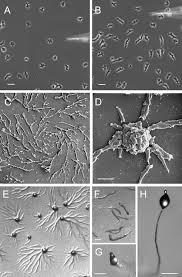
\includegraphics[width=0.6\linewidth]{./figs/Dictyostelida} 

}

\caption{Stages of Dictyostelium lifecycle. (A - B) Dictyostelium cells chemotaxing toward cAMP released from a micropipette. Cells that have not yet sensed cAMP are shown in (A). Within 1 or 2 min the cells polarize and migrate toward the source of chemoattractant (B). (C - D) Scanning electron micrograph of streaming Dictyostelium cells (C) and the formation of aggregates (D). (E) Formation of aggregation centers on an agar plate. (F) Slugs moving on an agar plate. (G) Culmination stage. (H) Fruiting body. Figure from Müller-Taubergen et al. 2012}\label{fig:Dictyostelium}
\end{figure}

\hypertarget{dissipative-zones}{%
\subsection{Dissipative zones}\label{dissipative-zones}}

In the reader of the Biodanza teacher training ``Module III Vital Unconsciousness and Biocentric Principle'' it is also mentioned that we live in a dissipative zone. Indeed, our whole globe can be seen as a large dissipative structure located in our solar system, which is a dissipative zone.

\begin{enumerate}
\def\labelenumi{\arabic{enumi}.}
\item
  There is an energy source, the sun that is radiating concentrated energy in photons.
\item
  Life forms are organising structure from the chaos of molecules on Earth by dissipating energy from the solar photons, light and UV, to heat through their organic pigments, e.g.~chlorophyll.
\item
  Animals, bacteria and fungi are secondary dissipative structures that are feeding on the concentrated chemical energy in the form of sugar, starch, proteins and fats that are produced by plants and cyanobacteria. They again dissipate energy in the form of heat through respiration.
\item
  The heat produced by life is dissipated to water and air and this induces tertiary dissipative processes like the water cycle, wind and sea currents etc.
\item
  Eventually heat is radiated to space, which acts as an energy sink.
\end{enumerate}

Because the temperature of Earth remains roughly stable, the same amount of energy is radiated to space under the form of heat as what comes in under the form of photons from the sun. As the energy content of heat is lower and more disperse it has a higher entropy than that of the incoming sunlight.
Because almost no mass is exchanged between Earth and space, mass has to be recycled and life is inherently cyclic.

This cyclic nature with its eternal reappearance is key for renewal and vitality, and has been recognized in all human cultures in their rich rituals that celebrate this cyclic origin. Biodanza also recognizes the importance of connecting and resonating with our cyclic origin. Indeed, biological regression in Biodanza is a moment of returning to, connecting with and the reappearance of our origin, which revitalize and initiates processes of renewal on a biological, physiological as well as on a psycho-socio-emotional level.

\newpage

\hypertarget{de-duve-a-biochemical-view-of-life}{%
\section{de Duve: a Biochemical View of Life}\label{de-duve-a-biochemical-view-of-life}}

In his Book ``Life Evolving - Molecules, Mind and Meaning'', \citet{deDuve2002} gave a very simple but brilliant definition of life:

Life is

\begin{enumerate}
\def\labelenumi{\arabic{enumi}.}
\tightlist
\item
  One,
\item
  Chemistry, and
\item
  Information
\end{enumerate}

In the following sections we will explore what de Duve meant with each component in his definition. Note, that each section starts with the key idea and then consists of more technical subsections that introduce the biological concepts in the reader ``Module IV Biological aspects of Biodanza'' in more detail.

\hypertarget{lifeOne}{%
\subsection{Life is One}\label{lifeOne}}

The first part in the definition of de Duve, ``Life is One'', has been instrumental for Rolando Toro when he coined the term ``Vital Unconsciousness''.

Life is one because all living organisms on earth

\begin{itemize}
\tightlist
\item
  are built of cells
\item
  evolved from the same ancestor
\item
  use the same molecule for storing, converting and using energy
\item
  use the same biological building blocks: lipids, sugars, amino acids for proteins and nucleic acids (DNA and RNA) to store our genetic information.
\end{itemize}

Readers who would like to skip technical details can immediately go to section \ref{lifeChemistry} Life is Chemistry.

\hypertarget{all-living-organisms-are-built-of-cells}{%
\subsubsection{All Living Organisms are Built of Cells}\label{all-living-organisms-are-built-of-cells}}

``Life is One'' because all organisms are composed of cells.
Green algae that can perform photosynthesis are a beautiful example of unicellular organisms. They were key for the development of life on our planet by releasing oxygen in our atmosphere (Figure \ref{fig:greenAlgae}).

\begin{figure}

{\centering 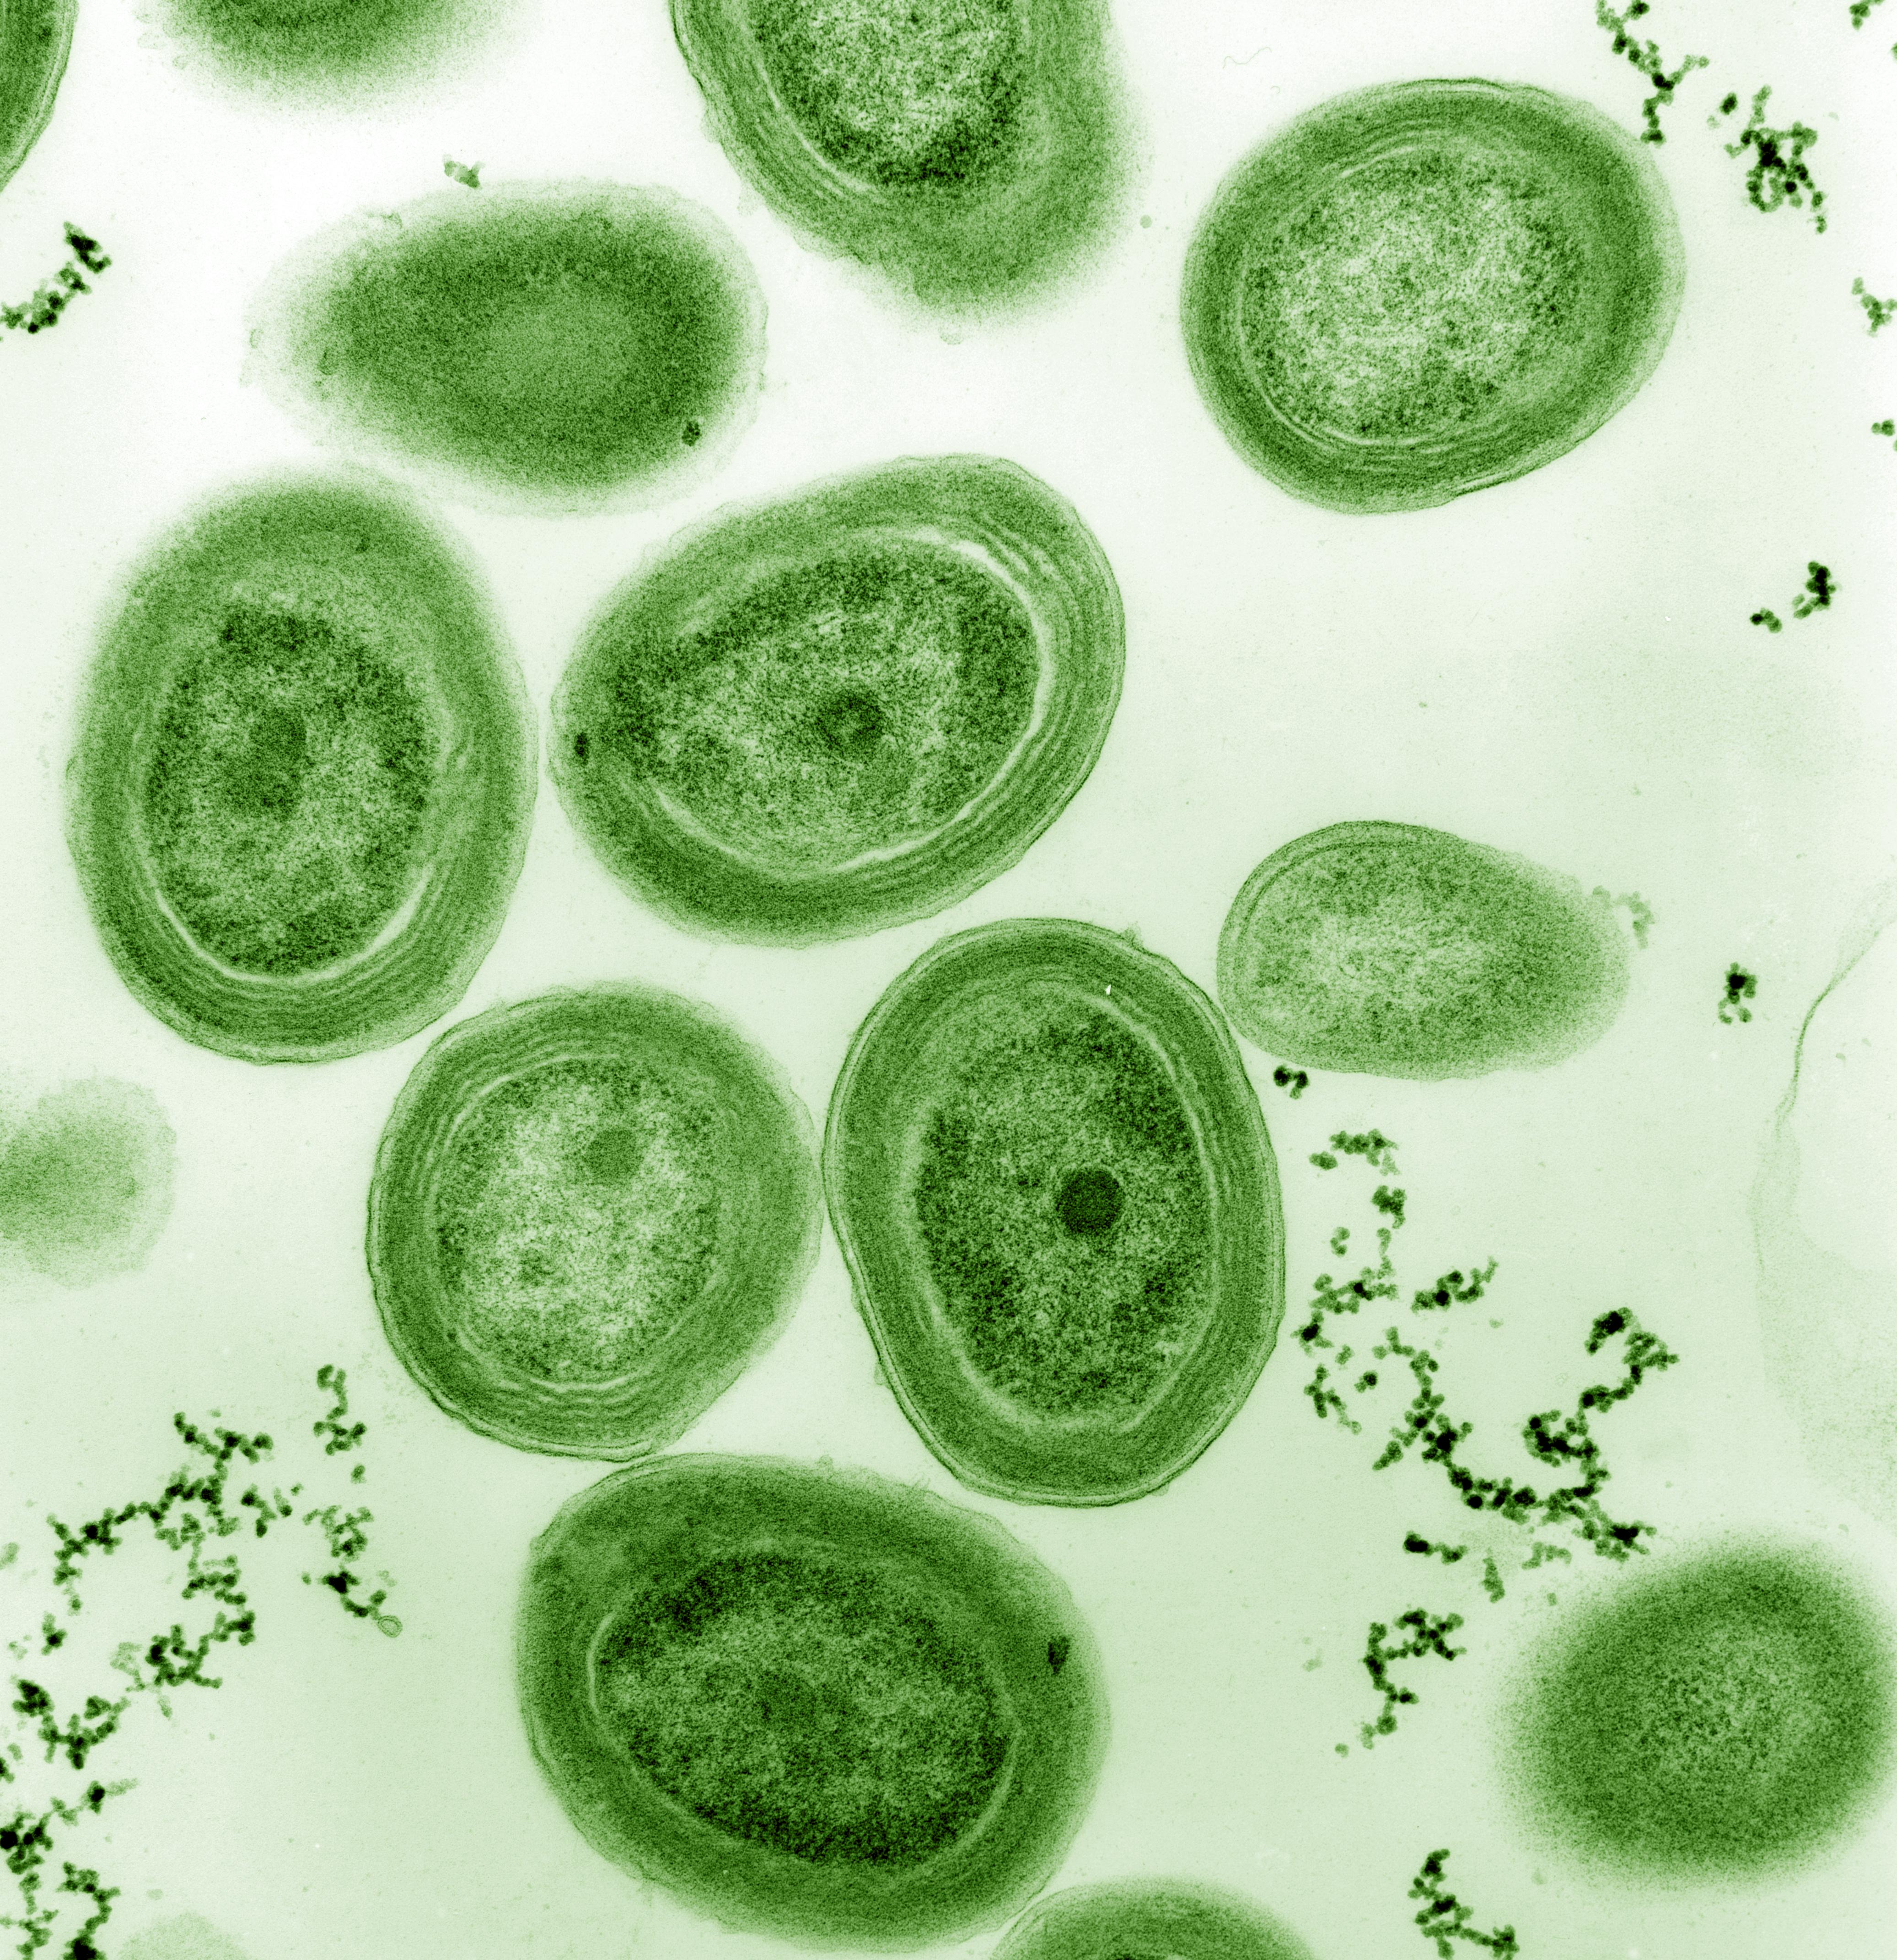
\includegraphics[width=0.3\linewidth]{./figs/Prochlorococcus_marinus} 

}

\caption{Cyanobacteria, unicellullar organisms that can perform photosynthesis. They were key in the development of life and radically changed Earth by releasing oxygen to our atmosphere (Source: Chisholm Lab, Wikipedia)}\label{fig:greenAlgae}
\end{figure}

A vital component of a cell is its membrane that is separating them from their environment while enabling them to interact with it and to concentrate chemicals inside the cell.

Multicellular organisms are composed of multiple cells. The cells are organised in
tissues, e.g.~spongy tissue in our bones or epithelium cells of our stomach; organs, e.g.~bones or our stomach; organ systems, e.g.~skeleton or digestive system; upto the organism. Figure \ref{fig:multiCellular} also shows how organisms are further organised in populations of organisms, ecosystems, and eventually our entire Biosphere. So ``Life is One'' because all living organisms consist of cells that are organised in large networks that work together.

\begin{figure}

{\centering 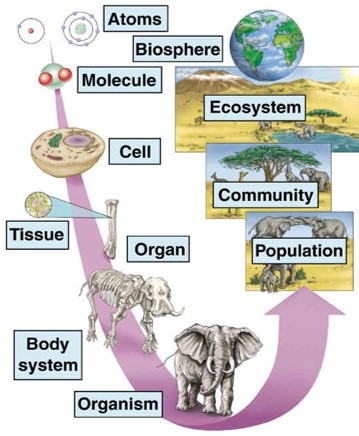
\includegraphics[width=0.3\linewidth]{./figs/organisationMulticellular} 

}

\caption{Multicellular organisms and biological organisation (Source: mrssmithsbiology)}\label{fig:multiCellular}
\end{figure}

\hypertarget{last-universal-common-ancestor}{%
\subsubsection{Last Universal Common Ancestor}\label{last-universal-common-ancestor}}

``Life is One'' because all species evolved from the same ancestral population of cells.
This is also referred to as the Last Universal Common Ancestor (LUCA). It is nicely indicated by the tree of life in Figure \ref{fig:treeOfLife}, which is one of the most important organising principles in biology. It shows the evolutionary relationships among different organisms and that all living beings eventually can be traced back to LUCA who is located at the root of the tree. Note, that the animal kingdom to which we belong is only a small branch in the tree.

\begin{figure}

{\centering 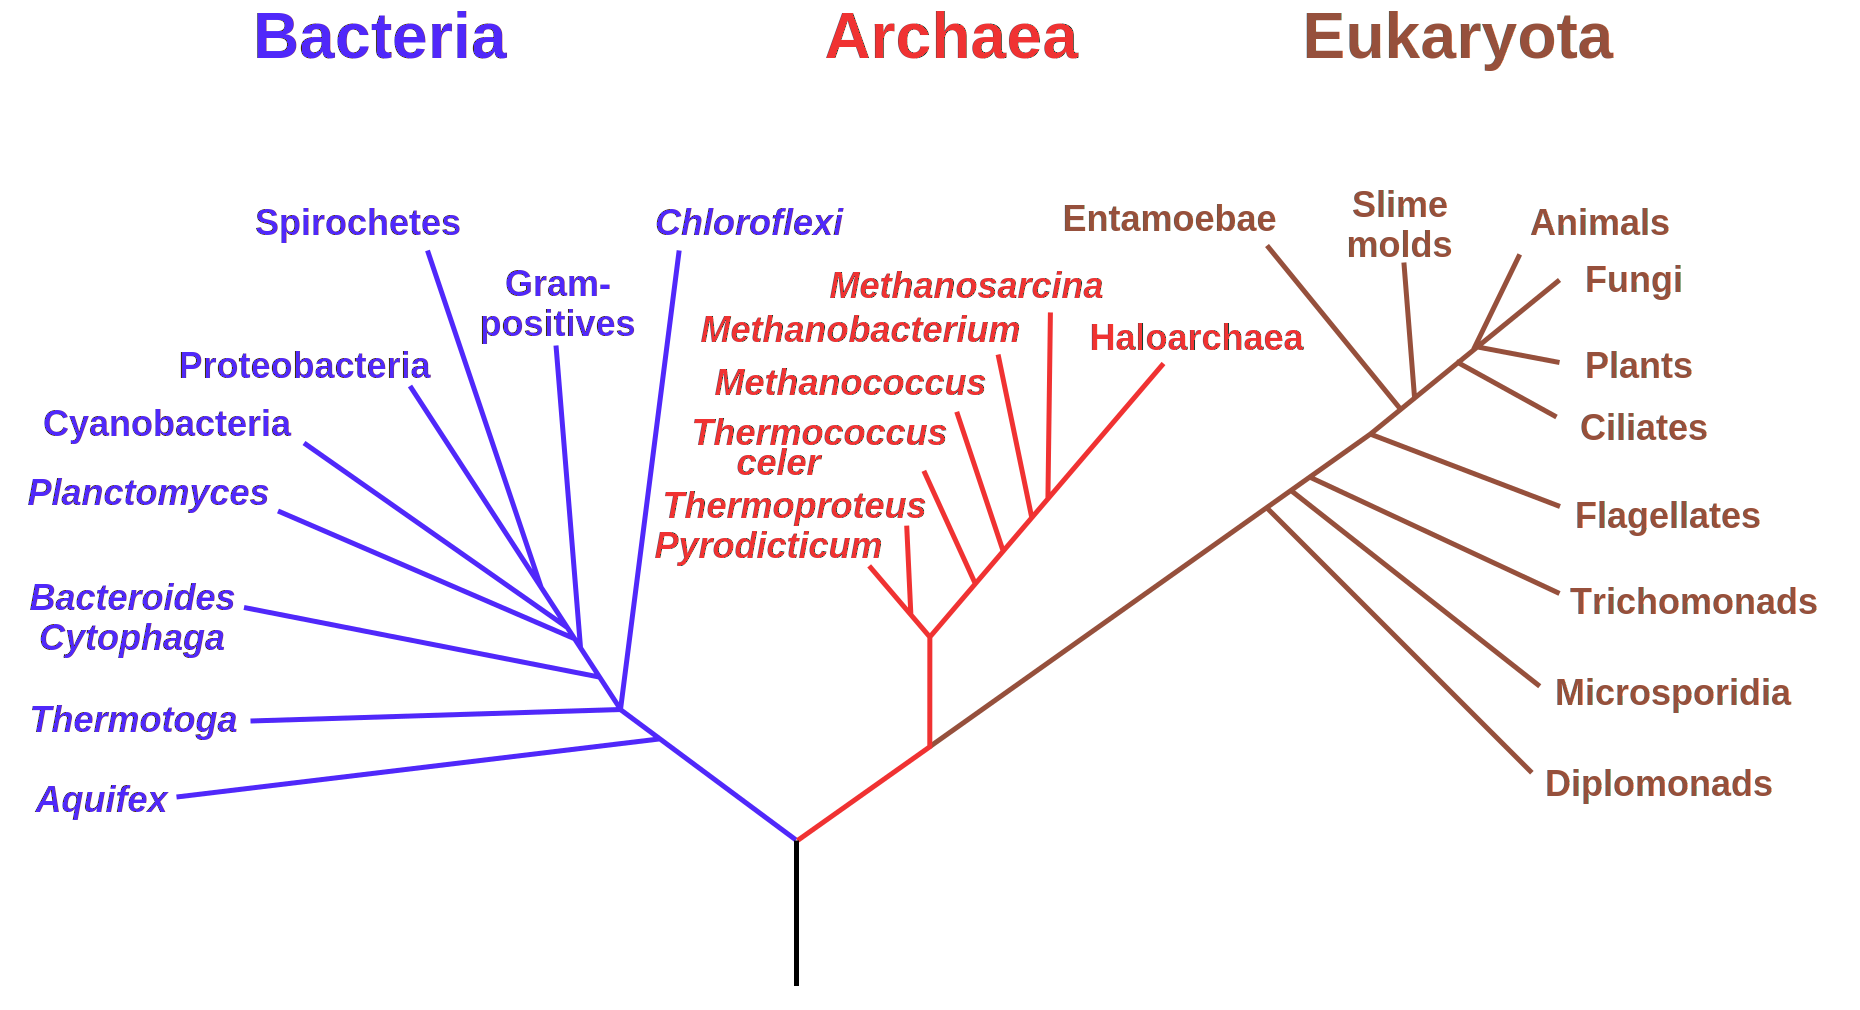
\includegraphics[width=0.8\linewidth]{./figs/Phylogenetic_tree} 

}

\caption{The tree of life is one of the most important organising principles in biology. It shows the evolutionary relationships among different organisms and also that all living beings eventually can be traced back to the last universal common ancestor (LUCA), who is located at the root of the tree (Source: Wikipedia)}\label{fig:treeOfLife}
\end{figure}

\newpage

\hypertarget{sectionEnergyCoin}{%
\subsubsection{Energy coin}\label{sectionEnergyCoin}}

``Life is One'' because all living organisms use the same ``energy coin'', the ATP-ADP system, to store and reuse energy.
Explained in technical terms, Adinosine-triphosphate (ATP) consists of a ribose sugar with 3 phosphate groups and a base adinine.
Splitting a phosphate group from adinosine-triphosphate (ATP) results in adinosine-diphosphate (ADP), a free phosphate group and energy.
The other way around, energy can be stored as chemical energy by binding a phosphate group to ADP.



\begin{figure}

{\centering 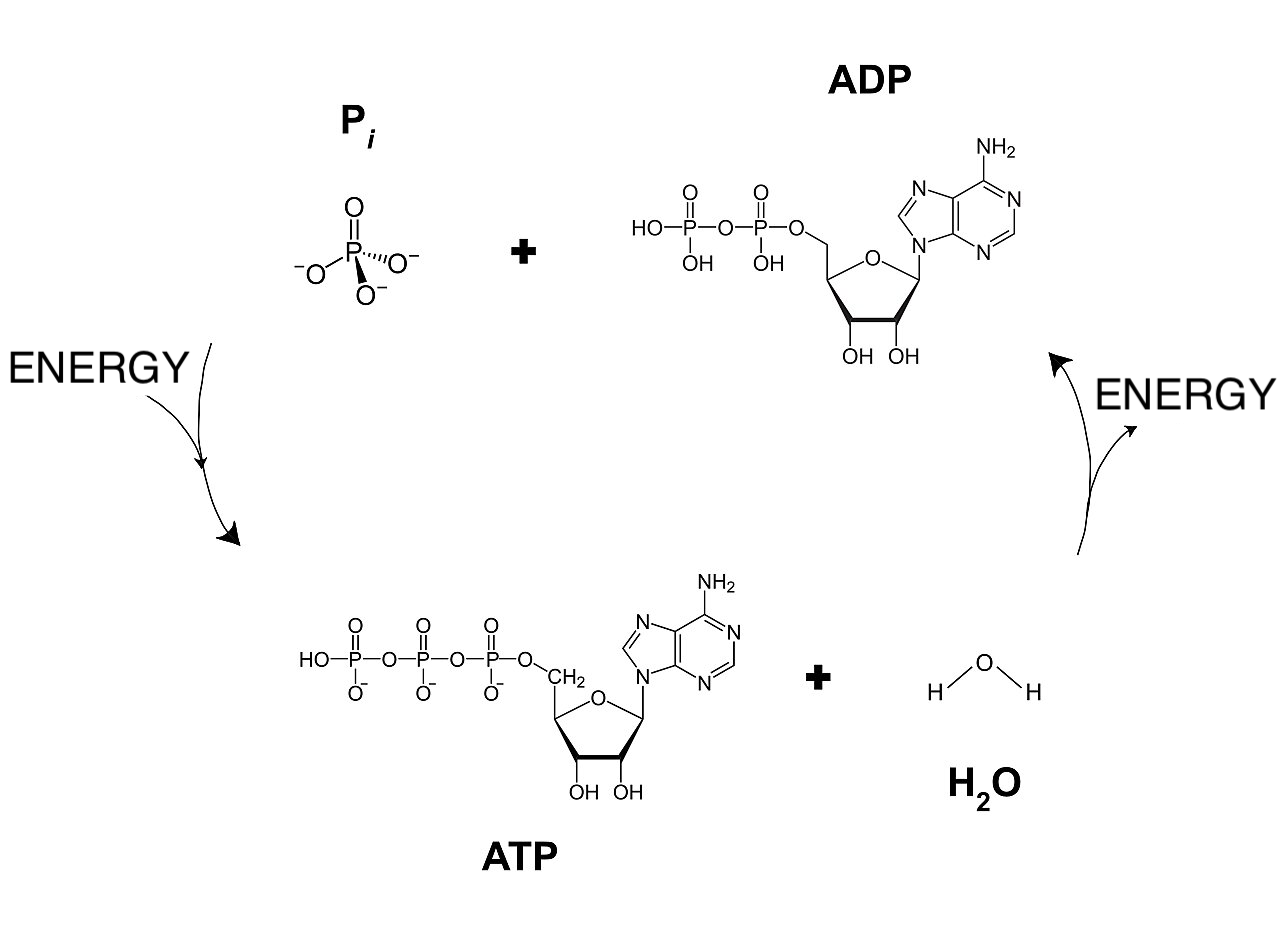
\includegraphics[width=0.7\linewidth]{./figs/ATP-ADP} 

}

\caption{Our energy coin ATP-ADP. Adinosine-triphosphate (ATP) consists of a base adinine, a ribose sugar and 3 phosphate groups. Splitting a phosphate group from adinosine-triphosphate (ATP) by a reaction with water (H\(_2\)O) results in adinosine-diphosphate (ADP), a free phosphate group and energy (Source: Adapted from Wikipedia)}\label{fig:atp-adp}
\end{figure}

Note, that ATP is also used to build RNA, an important molecule involved in storing, passing and expressing our genetic information (see Section \ref{sectionNucleicAcids} for more details on RNA). Indeed, ATP is incorporated in RNA upon splitting two phosphate groups. The resulting AMP (adinosine monophosphate) is one of the building blocks of RNA. So there is a close link between energy and genetic information!

\hypertarget{building-blocks-of-life}{%
\subsubsection{Building Blocks of Life}\label{building-blocks-of-life}}

``Life is One'' because all living organisms are composed of the same basic bio-molecules and we all know more than we think about them because we are what we eat!\\
Almost all molecules of living organisms are composed of

\begin{enumerate}
\def\labelenumi{\arabic{enumi}.}
\tightlist
\item
  Lipids, oil and fats, for storage and as building blocks for membranes,
\item
  Carbohydrates, sugars, for storing energy and as a backbone of large bio-molecules,
\item
  Amino acids, the building blocks of proteins, which are the workhorses of a cell, and
\item
  Nucleic Acids, building blocks of RNA and DNA, which are used to store and use the genetic information we inherit from our parents.
\end{enumerate}

Below, we focus on each of these building blocks in more detail.

\hypertarget{lipids}{%
\paragraph{Lipids}\label{lipids}}

\begin{figure}

{\centering 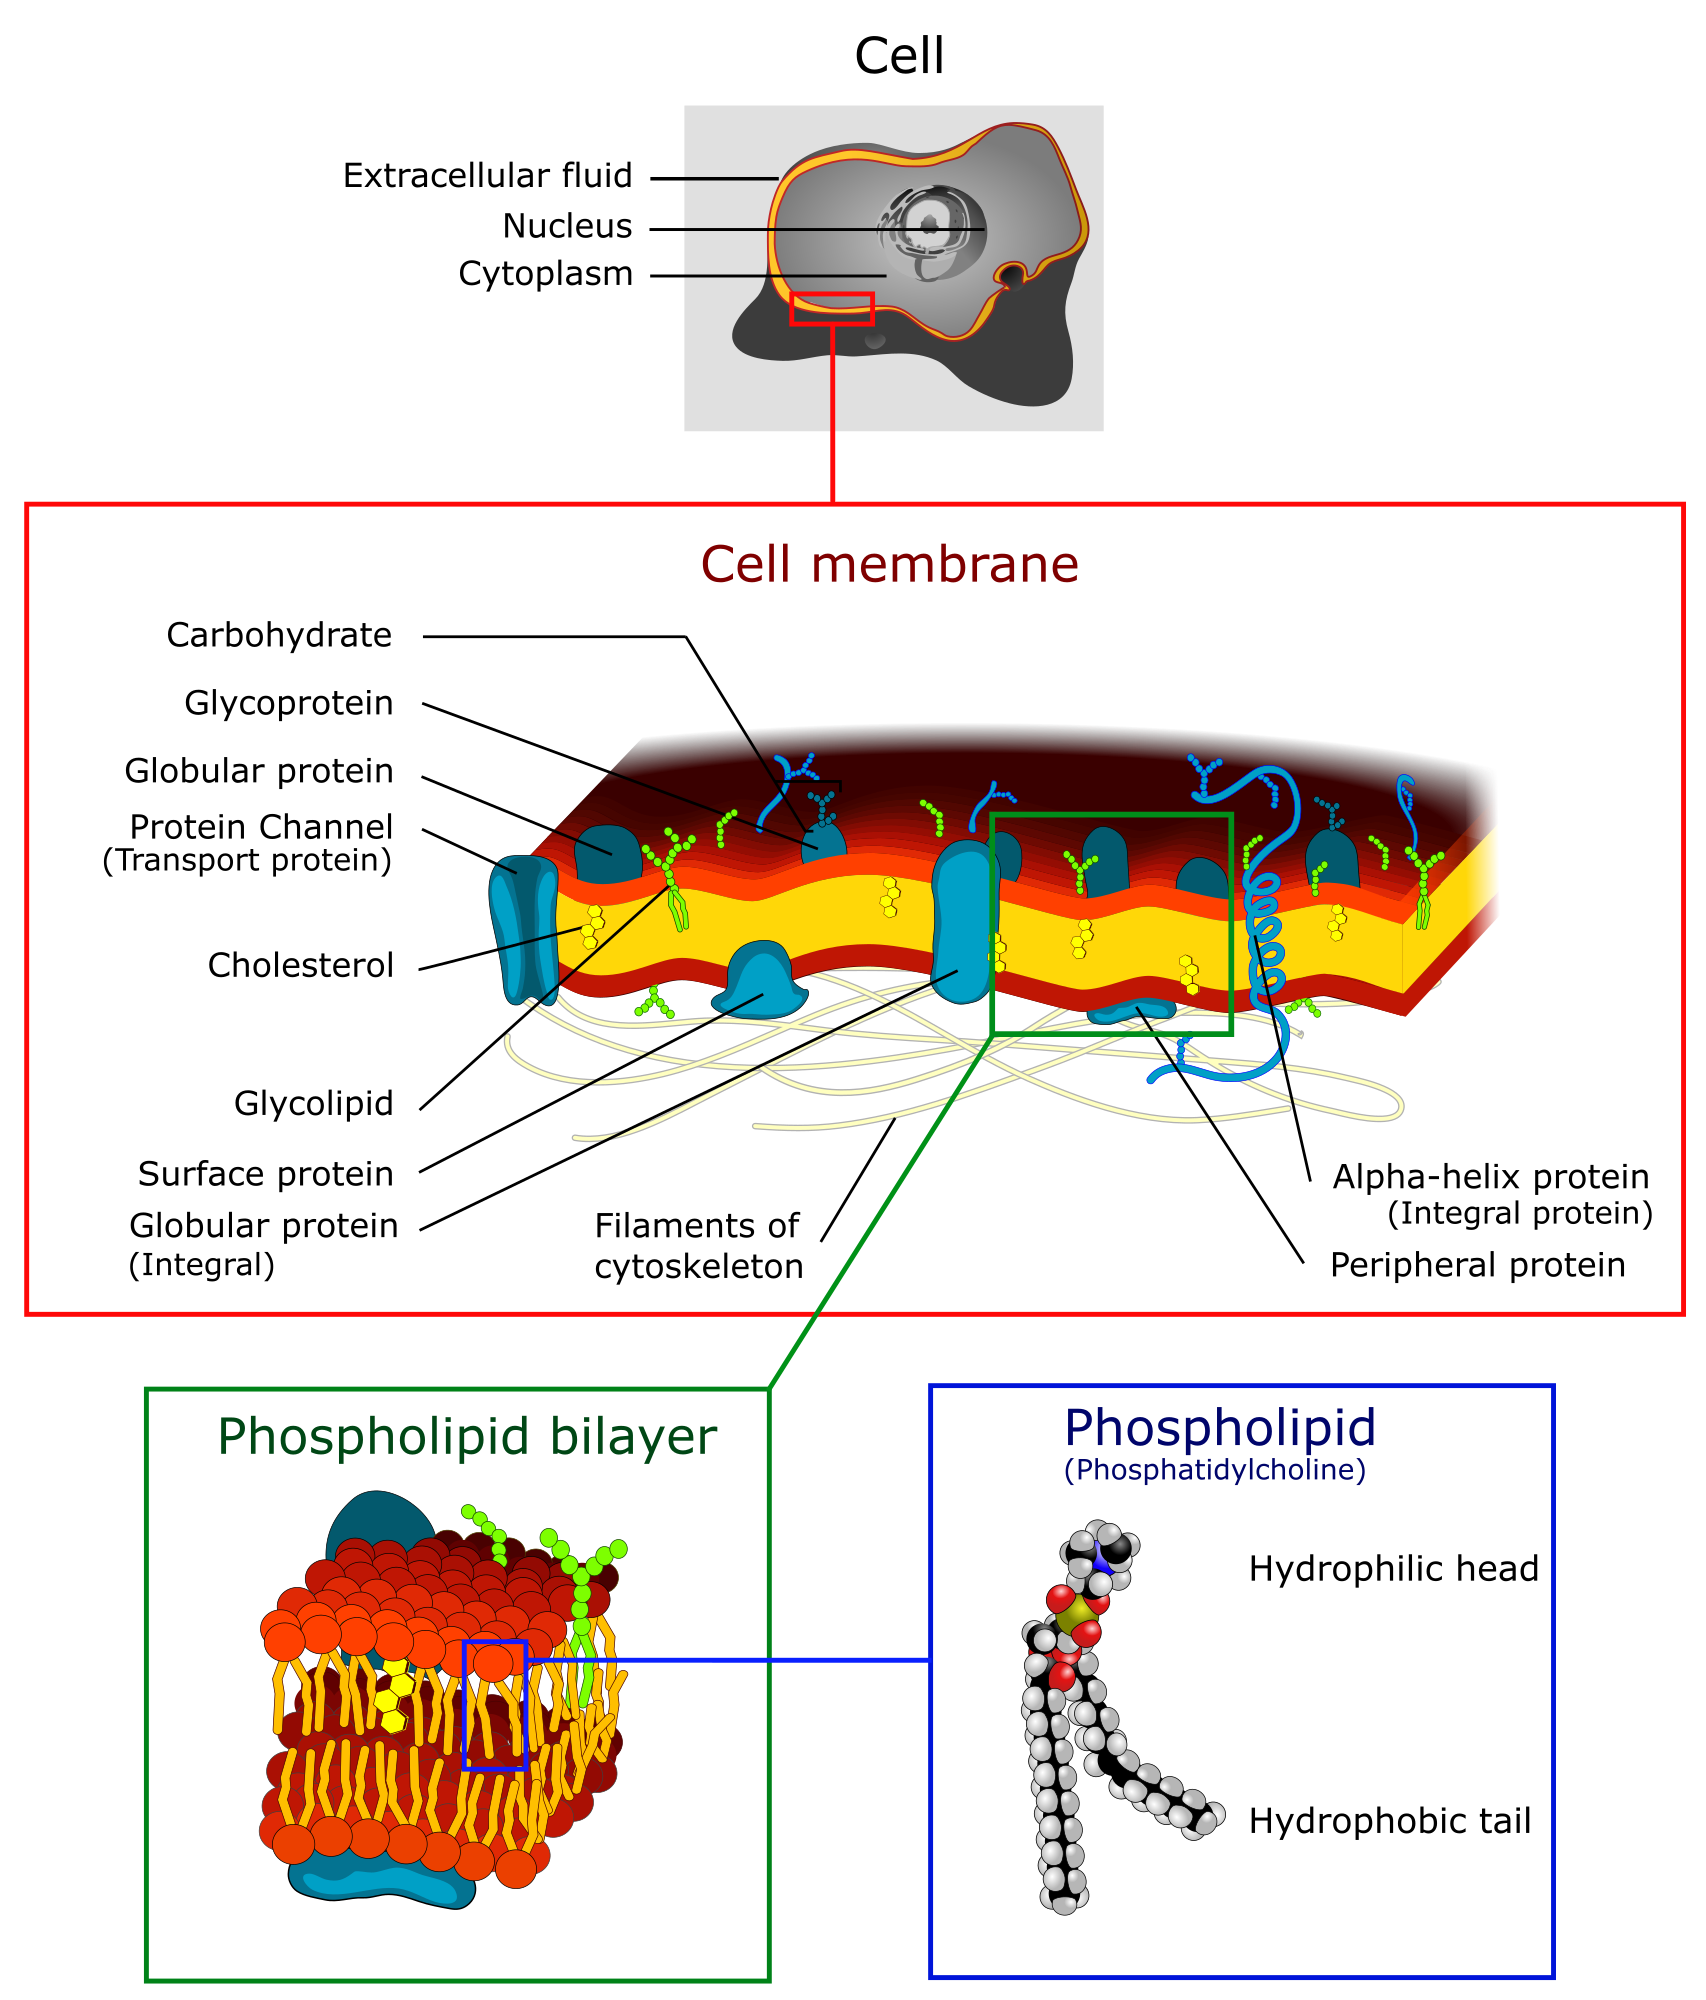
\includegraphics[width=0.8\linewidth]{./figs/Cell_membrane_detailed_diagram_4} 

}

\caption{Phospho-lipids have a very important role in life as they form membranes. Phospholipids have a hydrophilic head that likes to mix with water and long hydrophobic tails that do not mix with water. They sponteneously gives rise to bilayers in aqueous solutions similar to the structure seen in membranes. Membranes are the boundaries of the cell and they allow passivie diffusion of small molecules through their bilayer. Larger molecules can be actively exchanged with the environment through membrane proteins (Source: Doug Hatfield, Wikipedia)}\label{fig:lipids}
\end{figure}

Lipids, fats and oils, are used for storage. However, an important class of lipids, the phospholipids, make up membranes of cells and unicellular compartments called organelles see Figure \ref{fig:lipids}. Indeed phospholipids have a polar head that likes to be in water and a long apolar tail that does not mix with water. Therefore bilayers of phospholipid molecules are spontaneously formed in aqueous solutions.

Membranes provide the basis for concentrating specific molecules in (compartments of) living cells. This enable cells to build up a disequilibrium of chemical molecules that can perform work as a concentration gradient spontaneously dissipates toward its equilibrium value. So phospholipids are key for creating the boundary conditions necessary for cellular organization.

\hypertarget{carbohydrates}{%
\paragraph{Carbohydrates}\label{carbohydrates}}

Carbohydrates are important bio-molecules that are used for storage, energy and structure (Figure \ref{fig:carbohydrates}).

\begin{figure}

{\centering 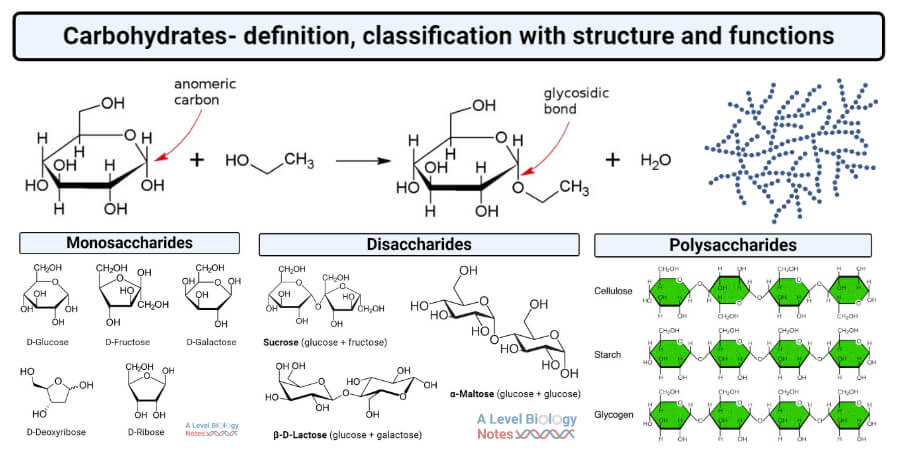
\includegraphics[width=1\linewidth]{./figs/Carbohydrates-definition-classification-with-structure-and-functions} 

}

\caption{Carbohydrates perform the important functions of storage, energy source and structure. They can be organised in biopolymers, long chains of carbohydrate molecules that are bound together. The polysaccharides starch and glycogen for instance are used to store energy by plant and animal cells, respectively. Cellulose, on the other hand, is a polysaccharide that gives plants structure. Deoxyribose and ribose are important carbohydrates that form the backbone of the biopolymers DNA and RNA, respectively. (Source: thebiologynotes.com)}\label{fig:carbohydrates}
\end{figure}

\begin{itemize}
\tightlist
\item
  Storage: glucose is stored inside animal cells using glycogen, a polymer of thousands of glucose molecules that are bound to each-other. Plants use a similar molecule, starch.
\item
  Energy source: specific proteins can split glycogen and starch into glucose that is subsequently metabolized for energy.
\item
  Structure: carbohydrates form the backbone of many bio-molecules, e.g.~long chains of desoxyribose and ribose act as the backbone of the bio-polymers DNA and RNA, respectively; and glucose is the backbone of cellulose, which give plants structure.
\end{itemize}

\hypertarget{amino-acids}{%
\paragraph{Amino Acids}\label{amino-acids}}

Amino acids by themselves are simple molecules (Figure \ref{fig:aminoAcids}).
Although hundreds of amino acids exist in nature, life is using only 20 of them and it is combining them in long molecules, polymers, which are referred to as proteins.
Proteins are hetero-polymers, consisting of the 20 amino acids that are arranged in long sequences that differ from protein to protein.
So unlike starch, that only consists of glucose molecules that are all identical, proteins are capable of carrying information.



\begin{figure}

{\centering 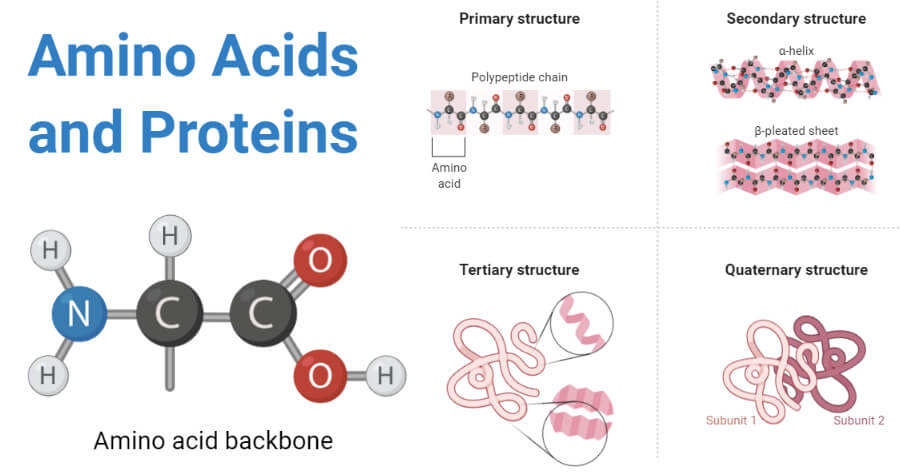
\includegraphics[width=1\linewidth]{./figs/Amino-acids-and-Proteins} 

}

\caption{Amino acids are simple molecules. They can be combined in long molecules, polymers, also known as proteins. Their long chain of amino acids spontaneously folds into a complex 3D structure from which their biological function emerges (Source: thebiologynotes.com)}\label{fig:aminoAcids}
\end{figure}

The crux of proteins is that their long chain of amino acids spontaneously folds into a complex 3D structure, which is determined by the properties and the specific sequence of its amino acids. From their complex and specific 3D structure their biological function emerges.

Indeed, many proteins work as a ``lock'' in which specific (bio)molecules fit as a ``key''. This enables proteins to bring molecules close together and to promote chemical reactions without being consumed. This process is also referred to as catalysis and proteins that perform catalysis are called enzymes, see Figure \ref{fig:enzyme}.

\begin{figure}

{\centering 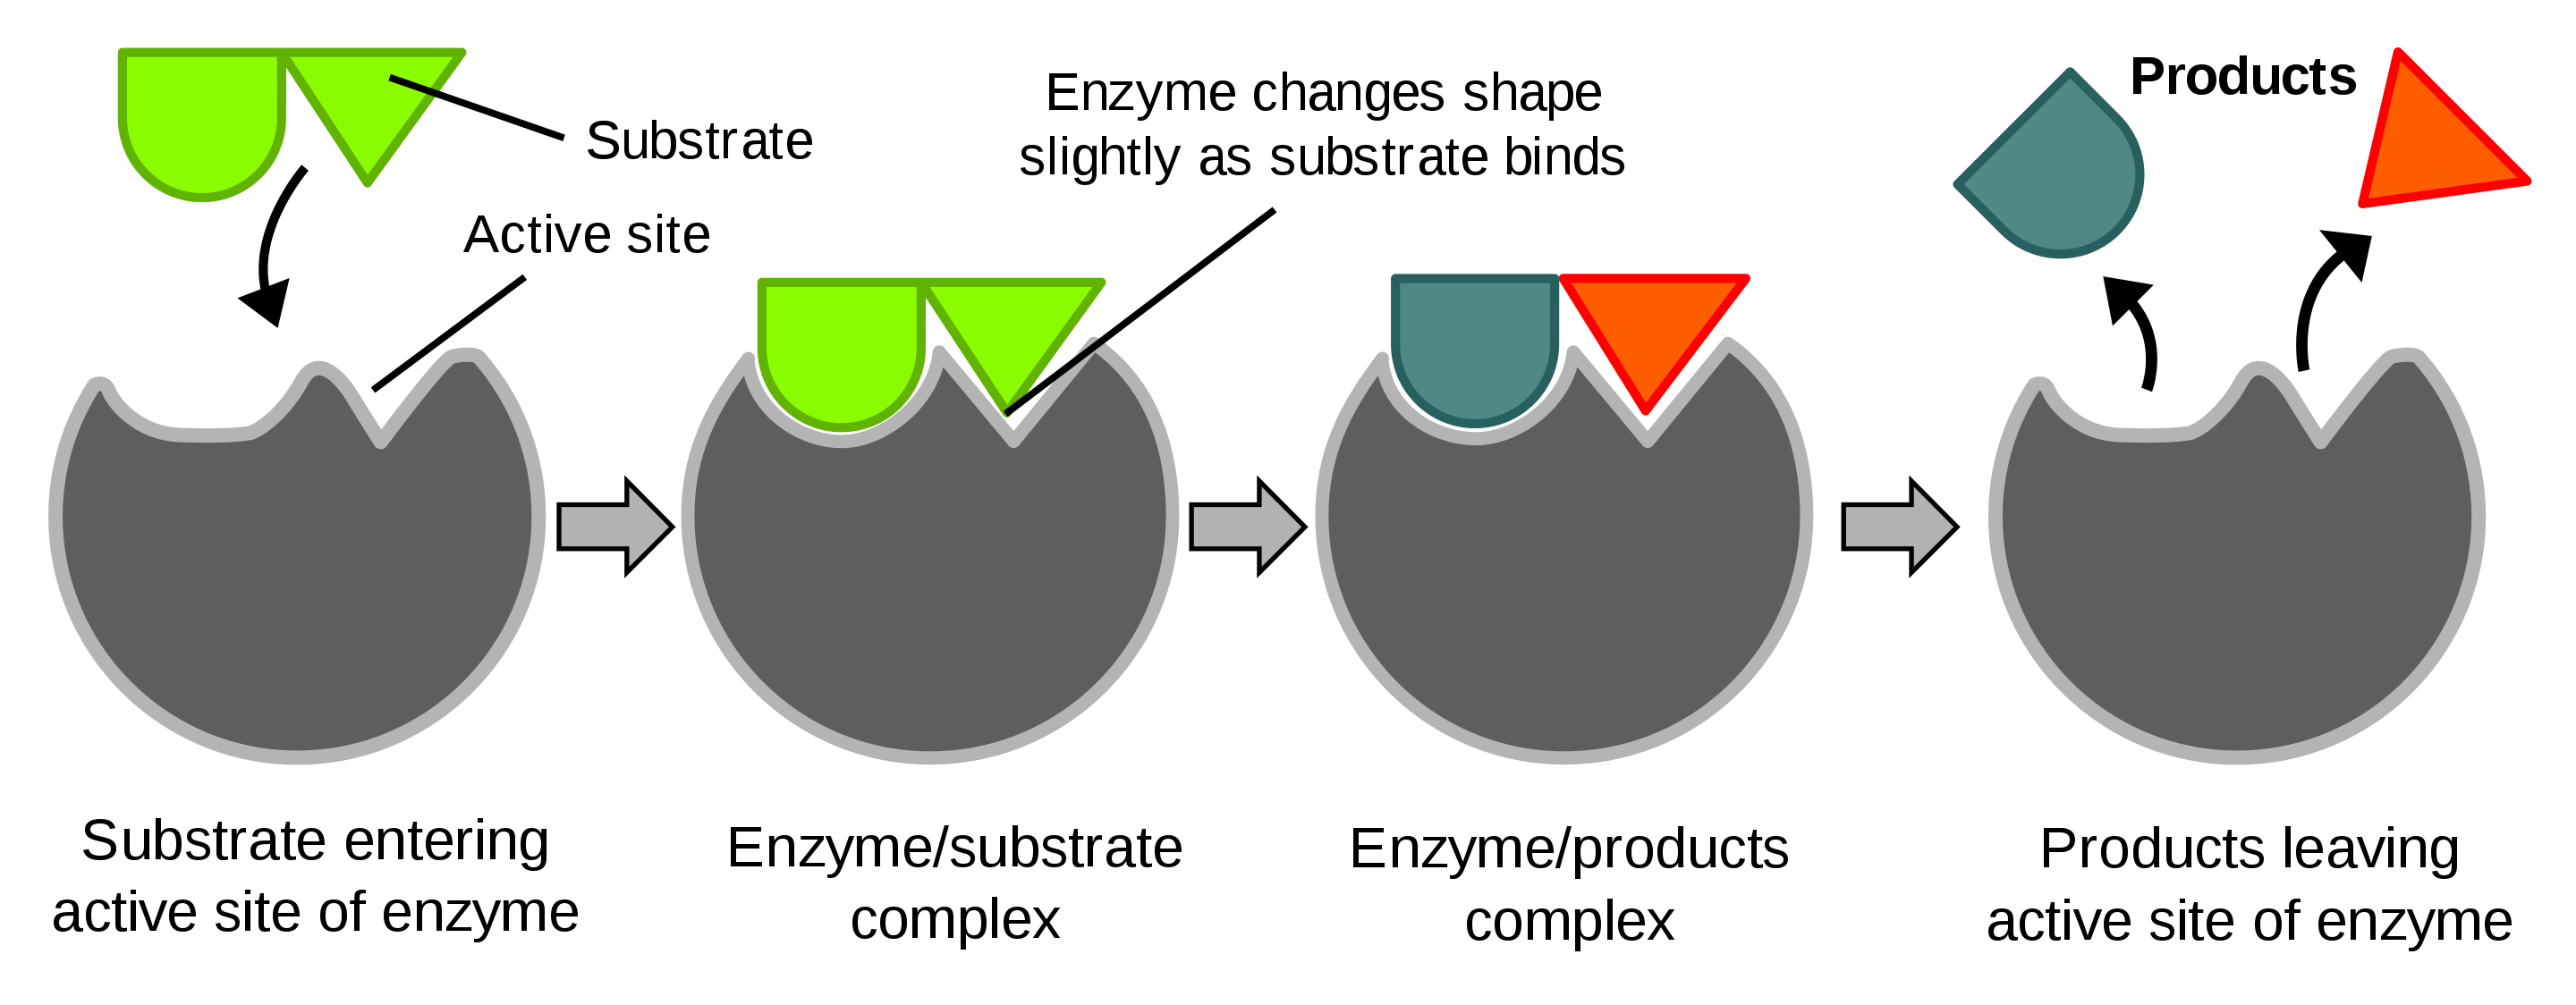
\includegraphics[width=0.5\linewidth]{./figs/EnzymePadlockKey} 

}

\caption{Diagram of a protein performing an enzyme action (Source: Wikipedia)}\label{fig:enzyme}
\end{figure}

Proteins are the main workhorses of the cell and they are important for moving food, digesting food, copying DNA, for giving the cell structure, affecting the rates at which other proteins work, etc\ldots{}

\newpage

\hypertarget{sectionNucleicAcids}{%
\paragraph{Nucleic Acids}\label{sectionNucleicAcids}}

Nucleic acids are build of nucleotides.
Each nucleotide is composed of one of four nitrogen-containing nucleobases, which carry the information

\begin{enumerate}
\def\labelenumi{\arabic{enumi}.}
\tightlist
\item
  cytosine {[}C{]},
\item
  guanine {[}G{]},
\item
  adenine {[}A{]} or
\item
  thymine {[}T{]} (DNA) or uracil {[}U{]} (RNA) ,
\end{enumerate}

a phosphate group and a sugar, i.e.~ribose in ribonucleic acid (RNA, Figure \ref{fig:RNA}) and deoxyribose in deoxyribonucleic acid (DNA, Figure \ref{fig:DNA}).

These nucleotides are the building blocks that are combined in long polymers: RNA and DNA.
DNA and RNA are hetero-polymers and the nucleotides conceptually can be combined in any order.
So they can contain information.
Indeed, they are key to store and use the genetic information we inherit from our parents.

DNA typically occurs as a double strand, where C and G, and, A and T hybridize to each other using respectively three and two hydrogen bridges to form the iconic double stranded helix structure, see Figure \ref{fig:DNA}.

There is a general consensus that life probably began by using RNA as information carrier.
DNA, however, is much more stable and lasts longer in water than RNA. Therefore, DNA probably emerged later and is now used to store the genetic information in most organisms.

Life is also one because we share the same genetic code, but we refer to Section \ref{lifeInformation} ``Life is Information'' for more details.

\begin{figure}

{\centering 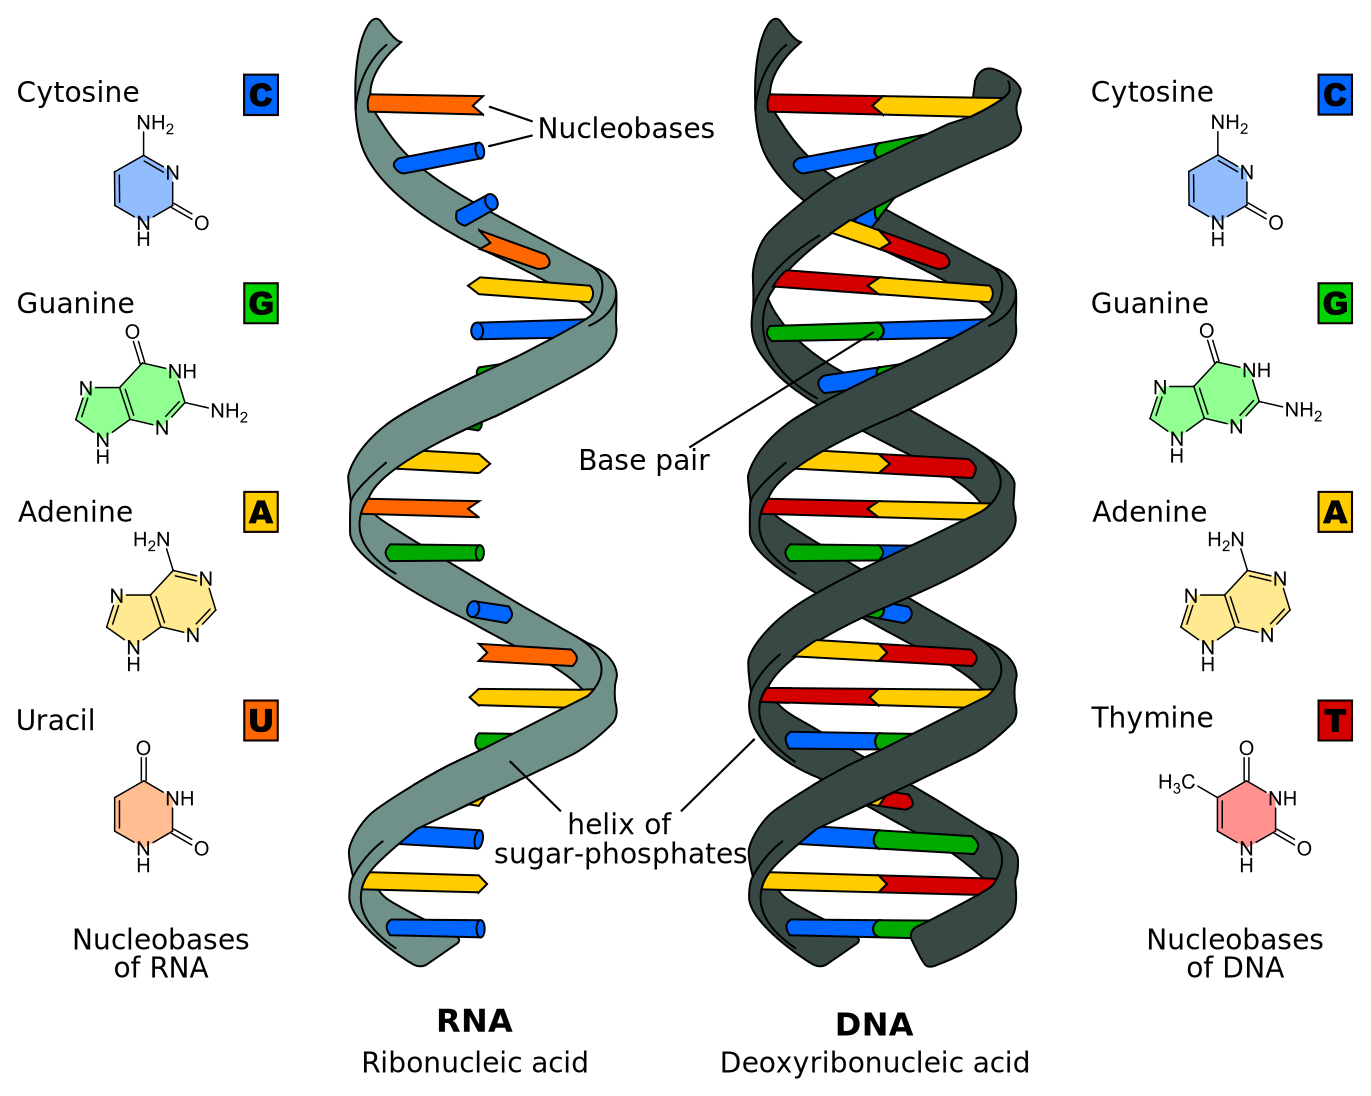
\includegraphics[width=0.5\linewidth]{./figs/Difference_DNA_RNA-EN} 

}

\caption{Nucleic acid: RNA (left) and DNA (right). RNA appears typically in a single strand and DNA as a double stranded molecule (Source: Wikipedia)}\label{fig:RNAvsDNA}
\end{figure}

\begin{figure}

{\centering 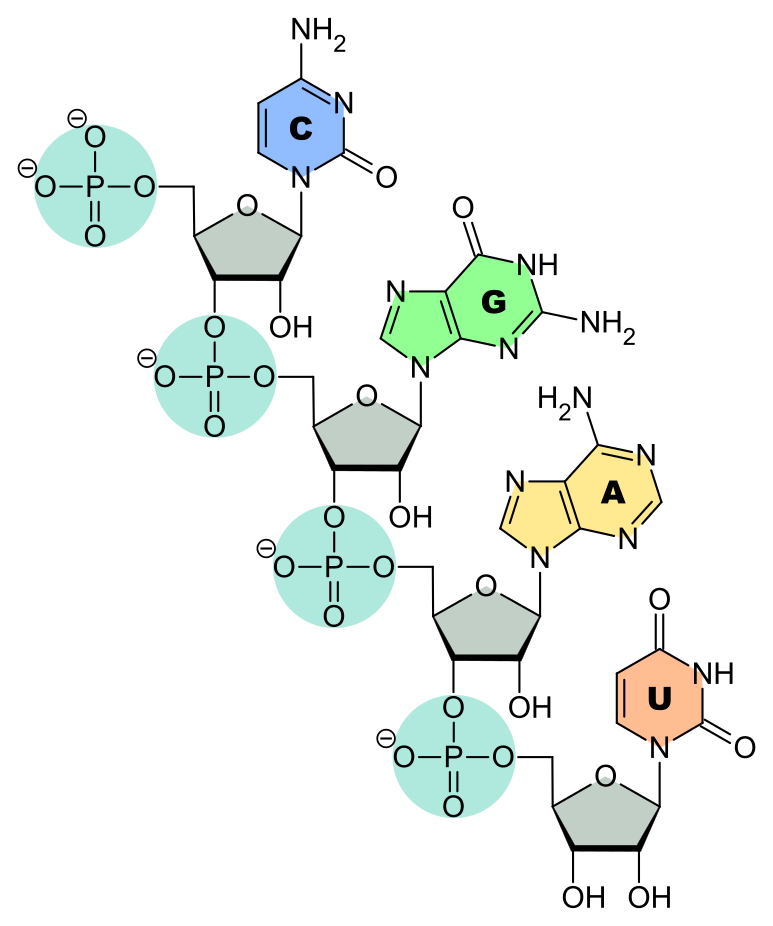
\includegraphics[width=0.5\linewidth]{./figs/RNA-Nucleobases} 

}

\caption{RNA is a polymeric molecule with various biological roles in coding, decoding, regulation and expression of genes. RNA consists of a chain of nucleotides. Each nucleotide is build from a ribose sugar that forms the backbone of the RNA  polymer, a phosphate group that is used to connect the ribose sugar molecules and a base adenine (A), cytosine (C), guanine (G) or uracil (U) that are the carriers of information. The bases can form hydrogen bonds between cytosine and guanine, between adenine and uracil, and, between adenine and thymine (a base from DNA) (Source: Adapted from Wikipedia)}\label{fig:RNA}
\end{figure}
\begin{figure}

{\centering 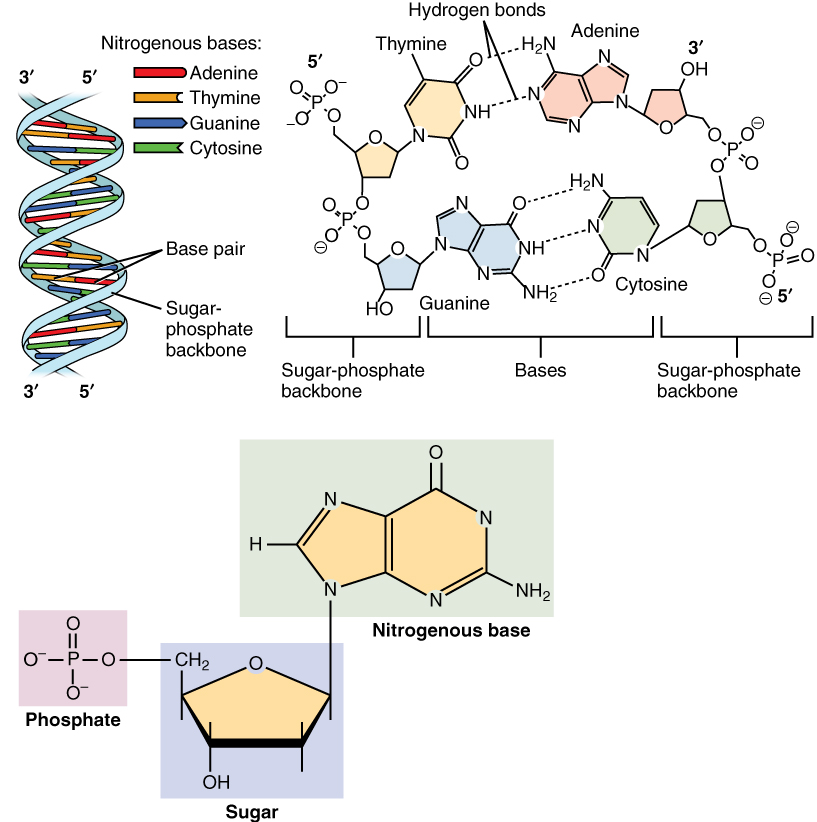
\includegraphics[width=0.5\linewidth]{./figs/DNA_Nucleotides} 

}

\caption{DNA is a polymer composed of two polynucleotide chains that coil around each other to form a double helix carrying genetic instructions for the development, functioning, growth and reproduction of all known organisms and many viruses. Each DNA single strand consists of a chain of nucleotides. Each nucleotide is build from a deoxyribose sugar that forms the backbone of the DNA  polymer, a phosphate group that is used to connect the deoxyribose sugar molecules and a base adenine (A), cytosine (C), guanine (G) or thymine (T) that are the carriers of information. The bases form hydrogen bonds between cytosine and guanine, and, adenine and thymine to assemble single stranded DNA in double stranded DNA. (Source: Wikipedia)}\label{fig:DNA}
\end{figure}

\newpage

\hypertarget{lifeChemistry}{%
\subsection{Life is Chemistry}\label{lifeChemistry}}

``Life is Chemistry'' because a cell consists of a complex network of chemical reactions that are connected to each other. Many feedback loops exist in this chemistry making it largely nonlinear. The feedback loops enables a cell to maintain in its regime or to switch from regime or attractor upon external and/or internal stimuli. An overview of most reactions in a living cell is given in Figure \ref{fig:chemicalReactionsCell}. I only included this overview to provide the reader with a sense of the complexity and the wealth of chemistry that takes place in each single cell. You can zoom in on this map on \url{http://biochemical-pathways.com/\#/map/1}.

\begin{figure}

{\centering 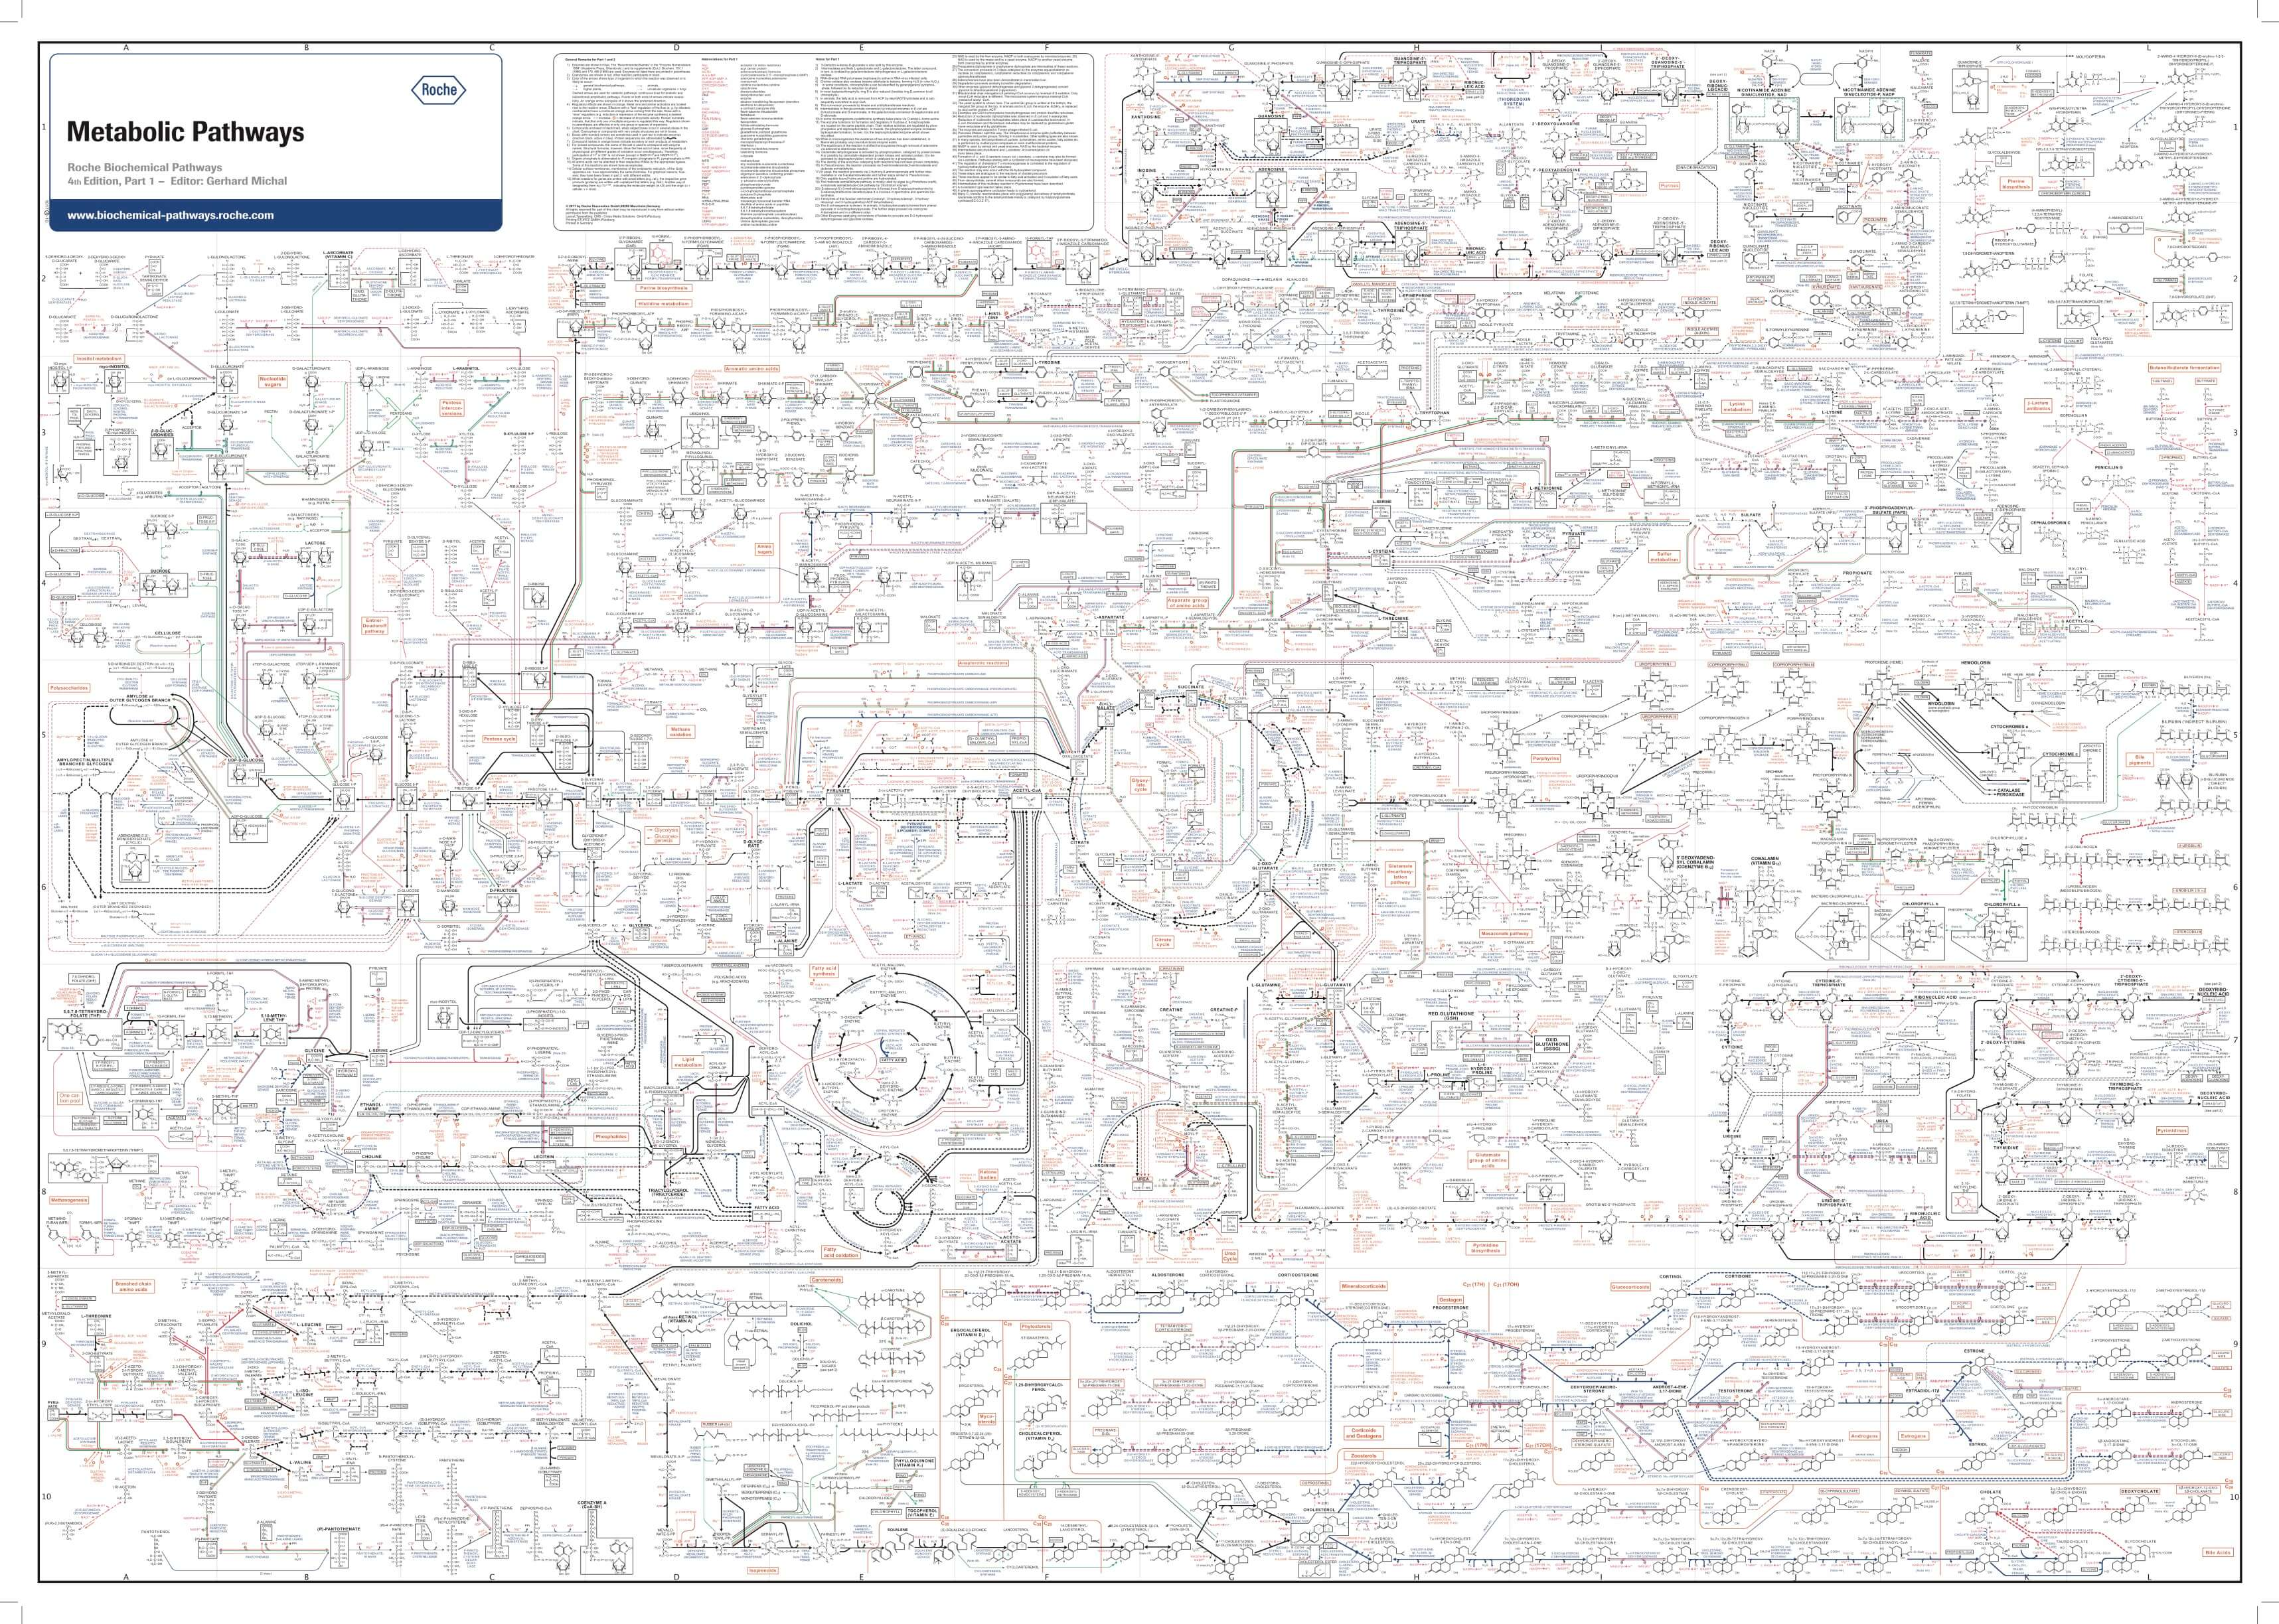
\includegraphics[width=1\linewidth]{./figs/roche_pathways} 

}

\caption{Network of the most important reactions in a living cell (Source: Dr. Gerhard Michal, Roche)}\label{fig:chemicalReactionsCell}
\end{figure}

In the remainder of this section we will introduce energy and catalysis in more detail, and we also give an intriguing example of how proteins play a role in the self-organisation of a cell. Readers who would like to skip technical details can immediately go to section \ref{lifeInformation} Life is Information.

\hypertarget{energy}{%
\subsubsection{Energy}\label{energy}}

``Life is Chemistry'' because it uses chemical reactions to store and use energy. See the ATP-ADP system in Section \ref{sectionEnergyCoin}

\hypertarget{catalysis}{%
\subsubsection{Catalysis}\label{catalysis}}

``Life is Chemistry'' because most chemical reactions are catalyzed, i.e.~initiated, promoted and made faster by proteins. The proteins facilitate the reaction without being used. The reactions would never take place if we would only mix the molecules at the concentrations that are typically occurring in a cell.

A catalyst is a chemical substance that helps a reaction to take place without being consumed. Proteins that are catalysts are also referred to as enzymes.

Enzymes are proteins that

\begin{itemize}
\tightlist
\item
  initiate the reaction
\item
  speed up the reaction and
\item
  make sure that the outcome is always the same.
\end{itemize}

Loosely speaking they are

\begin{itemize}
\tightlist
\item
  ``fishing'' certain molecules from the complex mixture in a cell,
\item
  which consists of thousands of chemical compounds generally at low concentrations,
\item
  through binding sites they can facilitate that these molecules (substrates) are getting close so that they can react and form a new compound.
\end{itemize}

These binding sites emerged from to the unique 3D structure of the protein. In Figure \ref{fig:enzyme} a schematic overview is given of the enzyme action of a protein.

In most cases enzymes work together in pathways, which consist of multiple chemical reactions for which (part of the) molecules produced in the previous reaction are used by another enzyme to facilitate the next reaction.

The Krebs cycle is a well known example. This pathway is the main source of energy for a cell through metabolising carbohydrates, lipids and/or proteins. The Krebs cycle is a cyclic pathway of multiple chemical reactions each catalyzed by another enzyme (see Figure \ref{fig:krebsCycle} or the you tube movie \url{https://www.youtube.com/embed/yk14dOOvwMk}).

The Krebs cycle is also used to generate building blocks for constructing certain nucleotides and amino acids.

\begin{figure}

{\centering 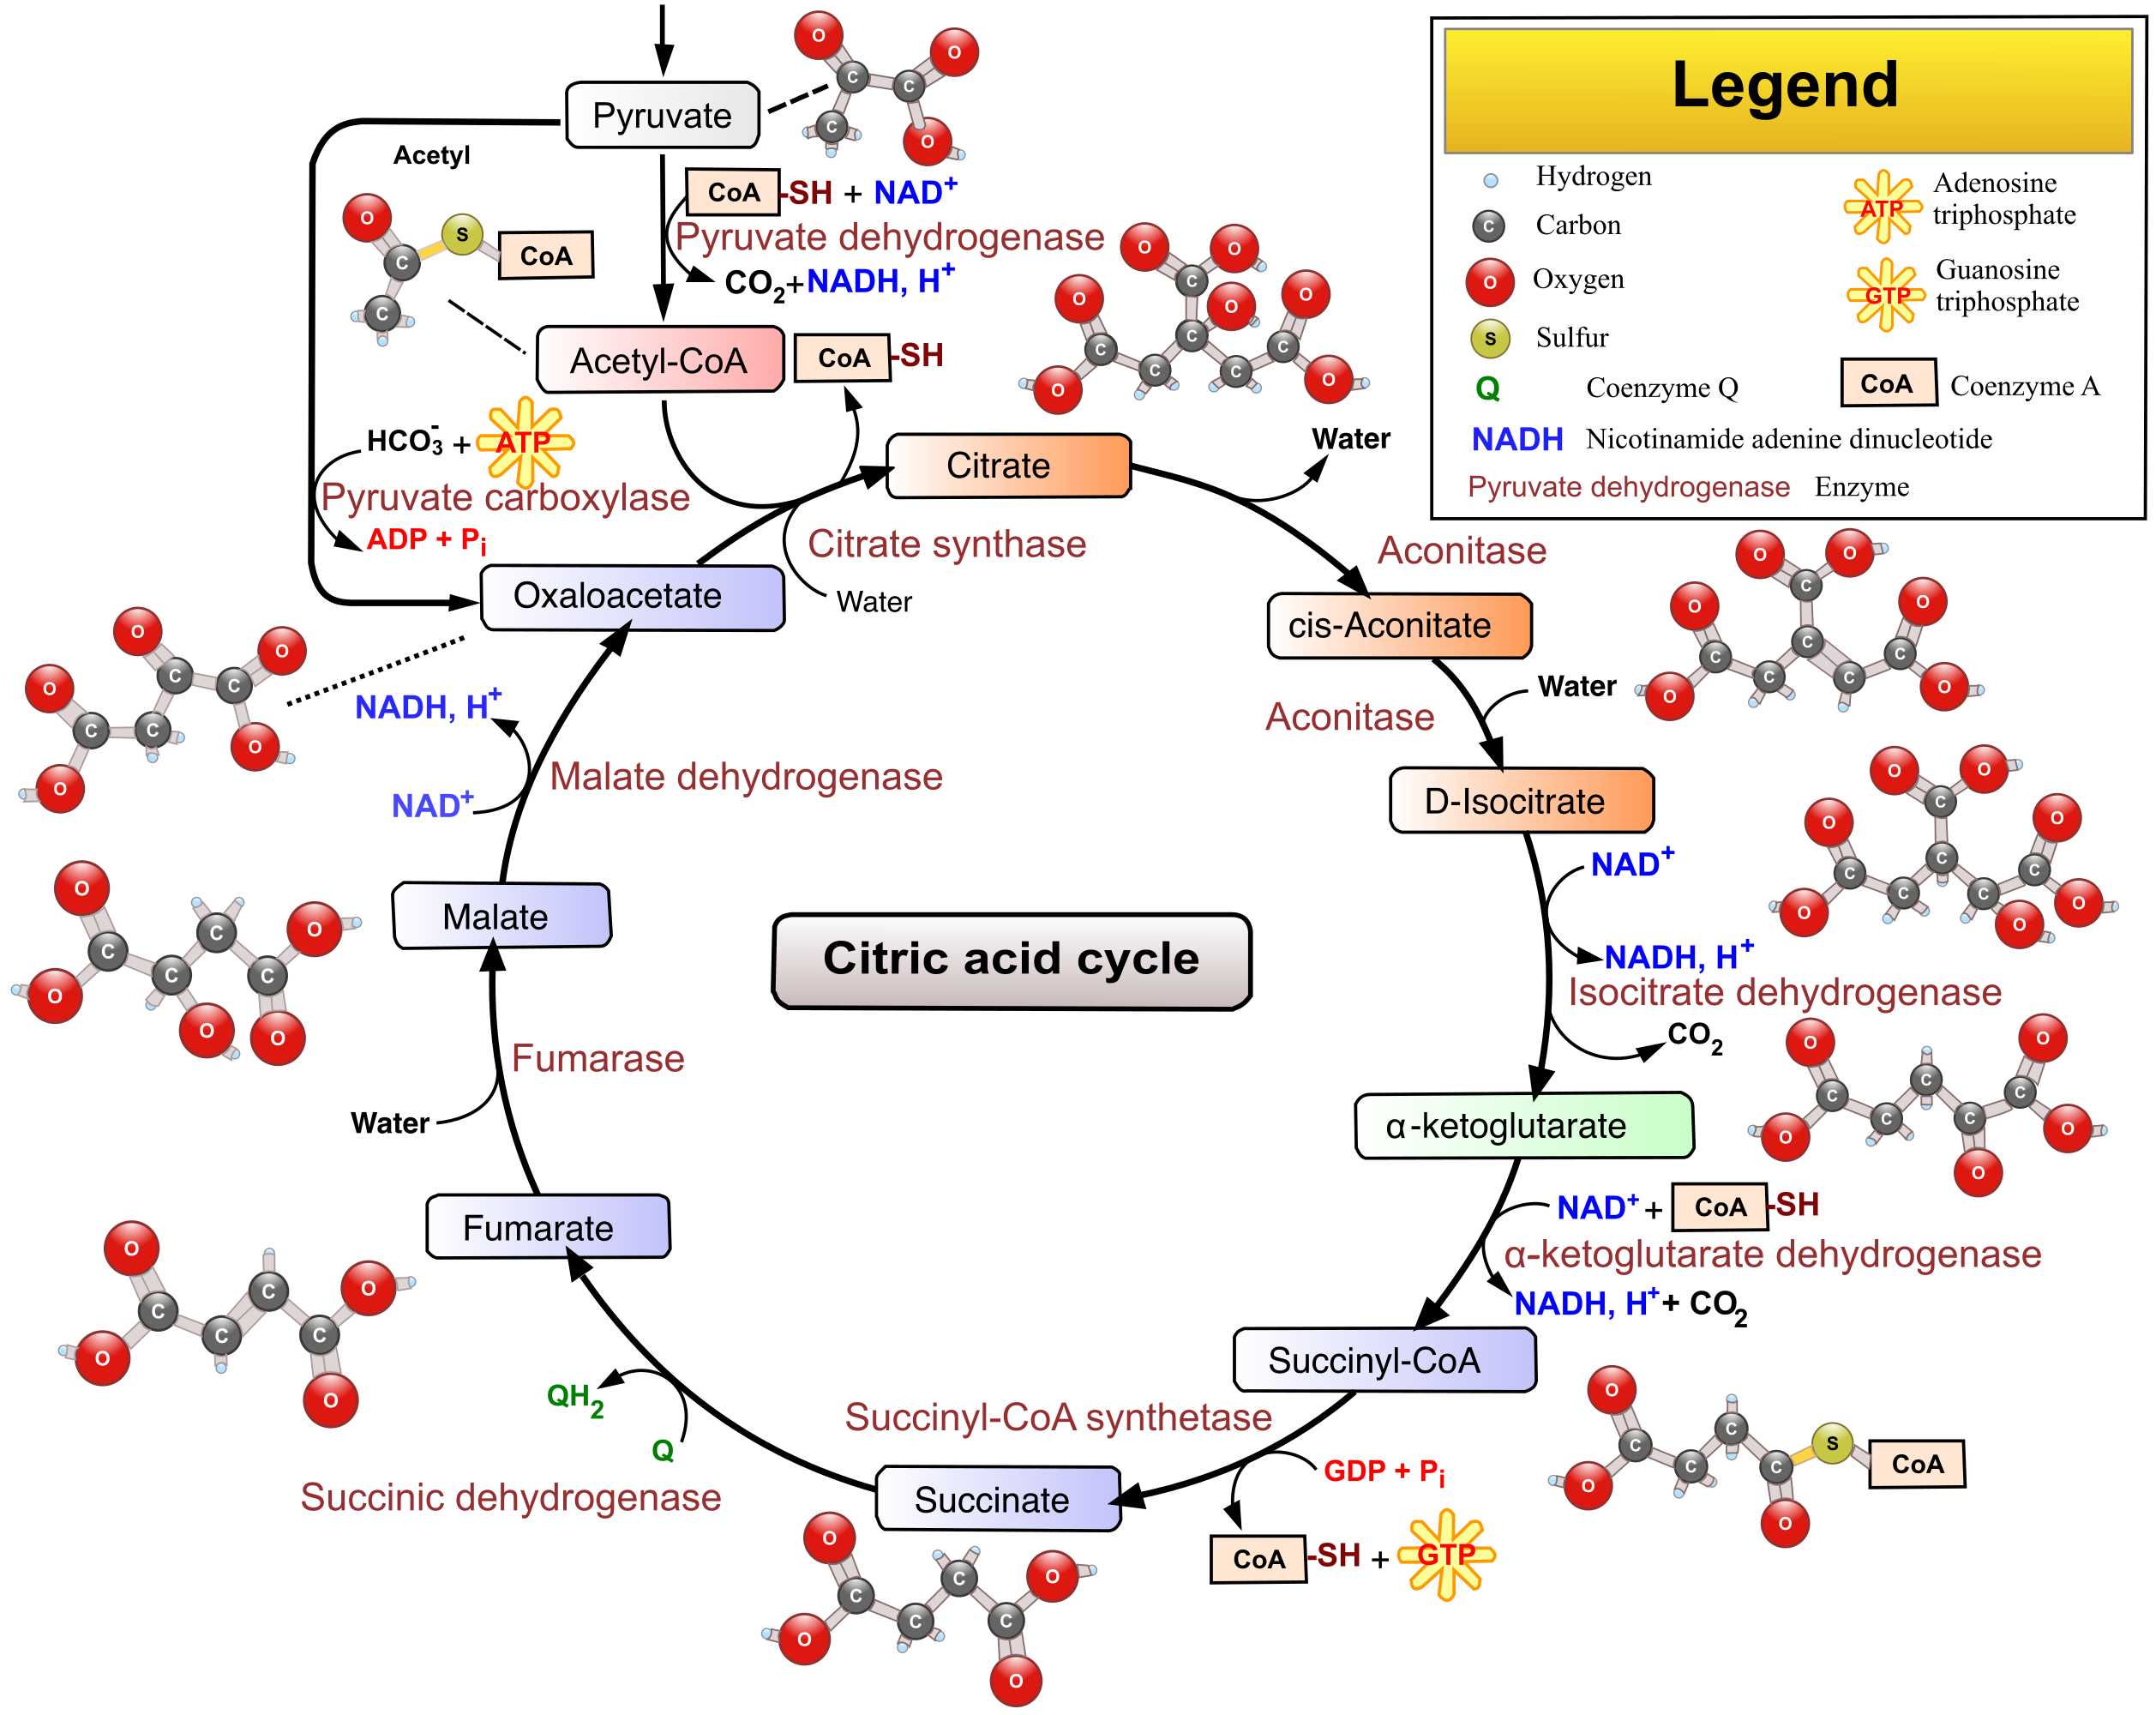
\includegraphics[width=0.7\linewidth]{./figs/Citric_acid_cycle_with_aconitate_2} 

}

\caption{Krebs cycle, a cyclic pathway connecting multiple reactions that provide the main source of energy for our cells by metabolising carbohydrates, proteins and lipids. Each reaction is catalised by an enzyme  (Source: Narayanese, Wikipedia)}\label{fig:krebsCycle}
\end{figure}

We can end this section with a quote of \citet{deDuve2002}: ``Any living organism is a reflection of its enzyme arsenal''.

\newpage

\hypertarget{self-organisation}{%
\subsubsection{Self-Organisation}\label{self-organisation}}

Life is also characterized by its ability for self-organisation. Some proteins are also important to give structure to a cell and they can spontaneously form structure.
An intriguing illustration of self-organisation is provided by \citet{Cheng2019} who
homogenized Xenopus laevis egg cell cytoplasma extracts, i.e.~the liquid with structures from the cell, and showed that the homogeneous extract spontaneously reorganized itself in cell like structures in a matter of minutes (see Figure \ref{fig:selforganisation} and you tube movie \url{https://www.youtube.com/embed/prq1Occu22s}).



\begin{figure}

{\centering 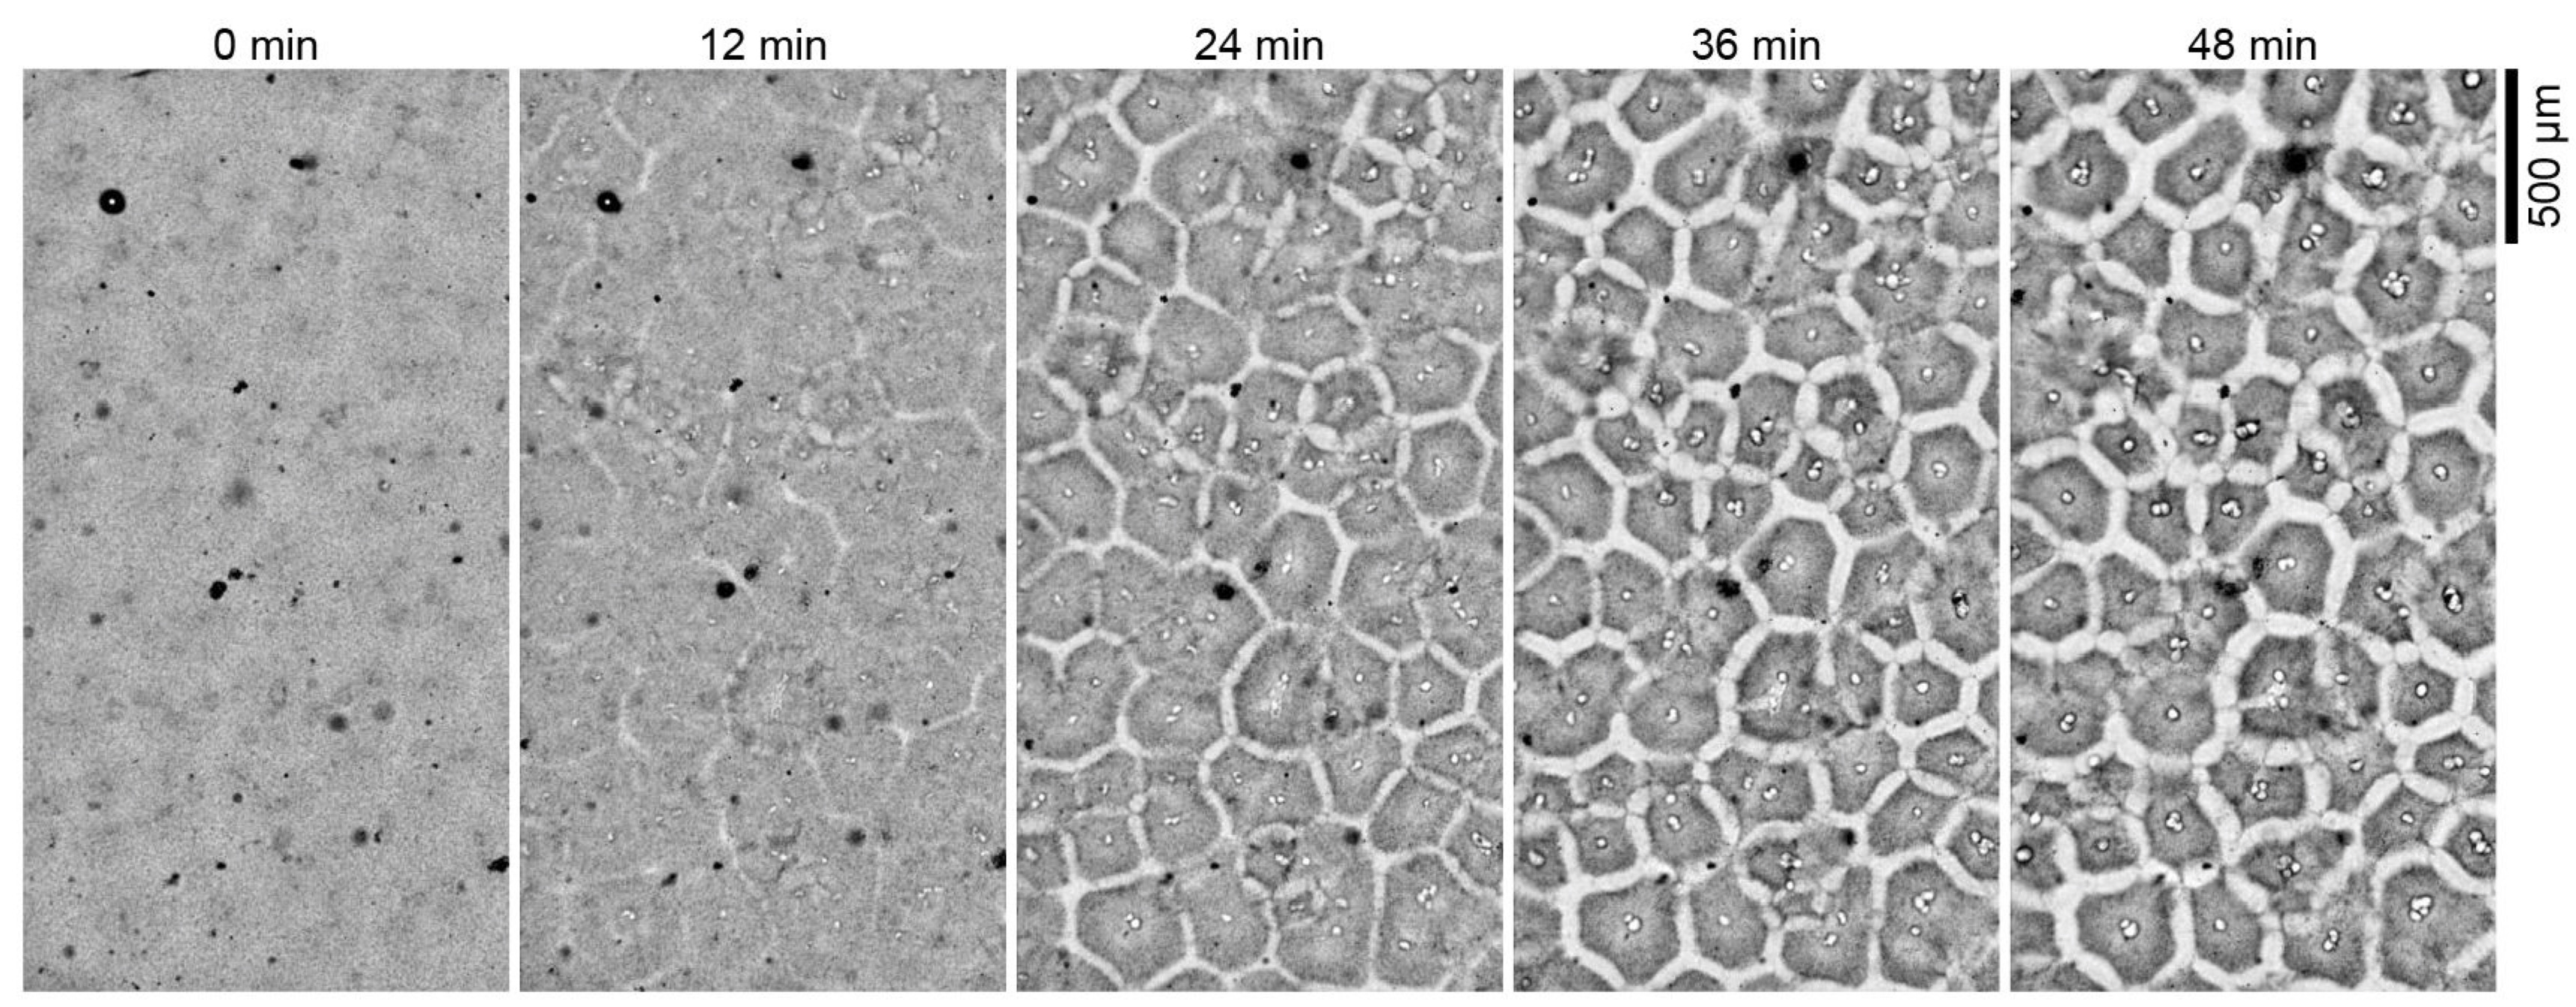
\includegraphics[width=1\linewidth]{./figs/selforganisation} 

}

\caption{Homogenized Xenopus laevis egg cytoplasmic extracts spontaneously organized into cell-like compartments \citep{Cheng2019}}\label{fig:selforganisation}
\end{figure}

\citet{Cheng2019} found that ATP, the energy currency of a cell; microtubuli, a kind of filamentous proteins; and dynein, a kind of motor protein, were required and driving this process of self-organisation.

\begin{figure}

{\centering 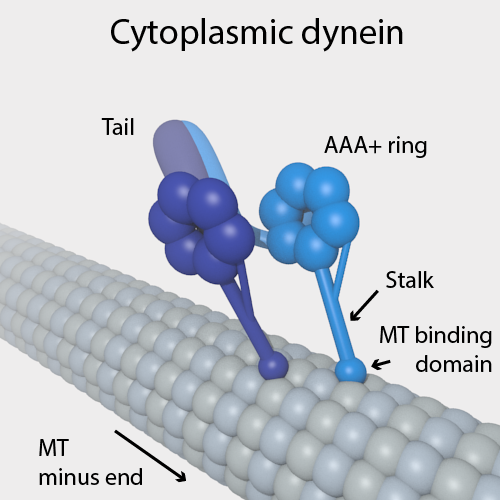
\includegraphics[width=0.3\linewidth]{./figs/DyneinHeavyChainOnMT} 

}

\caption{Microtubulus (long filamentous protein) with Dynein "motor" protein attached (Source:  Wikipedia)}\label{fig:dynein}
\end{figure}

Note, that proteins thus play a central role in life. They are key for catalysis and giving structure. Hence, a cell thus not only inherits genetic information, but, also its spatial organisation from a mother cell!

\newpage

\hypertarget{lifeInformation}{%
\subsection{Life is Information}\label{lifeInformation}}

Our genetic information to build all our bio-molecules, which we inherit from our parents, is stored in our DNA. DNA is a hetero-polymer or a long chain of 4 different building blocks, nucleotides. So the genetic information is stored in an alphabet of 4 letters. This is
adenine (A), cytosine (C), guanine (G) and thymine (T) for DNA.

It makes no physical or chemical difference what the identity of the next nucleotide is in the DNA chain. So our DNA can be seen as a coding system to store and pass genetic information from one generation to the next. Life is therefore also information and not only chemistry.

In the reminder of this section we will focus on the flow of information in a cell in more detail. Readers who would like to skip technical details can immediately go to section \ref{maturanaVarela} Maturana and Varela: a Systems View of Life.

\hypertarget{the-central-paradigm-of-molecular-biology}{%
\subsubsection{The central paradigm'' of molecular biology}\label{the-central-paradigm-of-molecular-biology}}

The ``central paradigm'' of molecular biology states that the sequence of nucleotides in DNA are first \emph{transcribed} into RNA and then \emph{translated} into proteins, see Figure \ref{fig:centralParadigm}.

Note, that some RNA molecules are also end products. Indeed RNA can also have a catalytic function, i.e.~initiate and promote chemical reactions without being consumed.

A \emph{gene} is the unit of genetic material, a DNA sequence that is encoding for the synthesis of a gene product, either a protein or a functional RNA.

\begin{figure}

{\centering 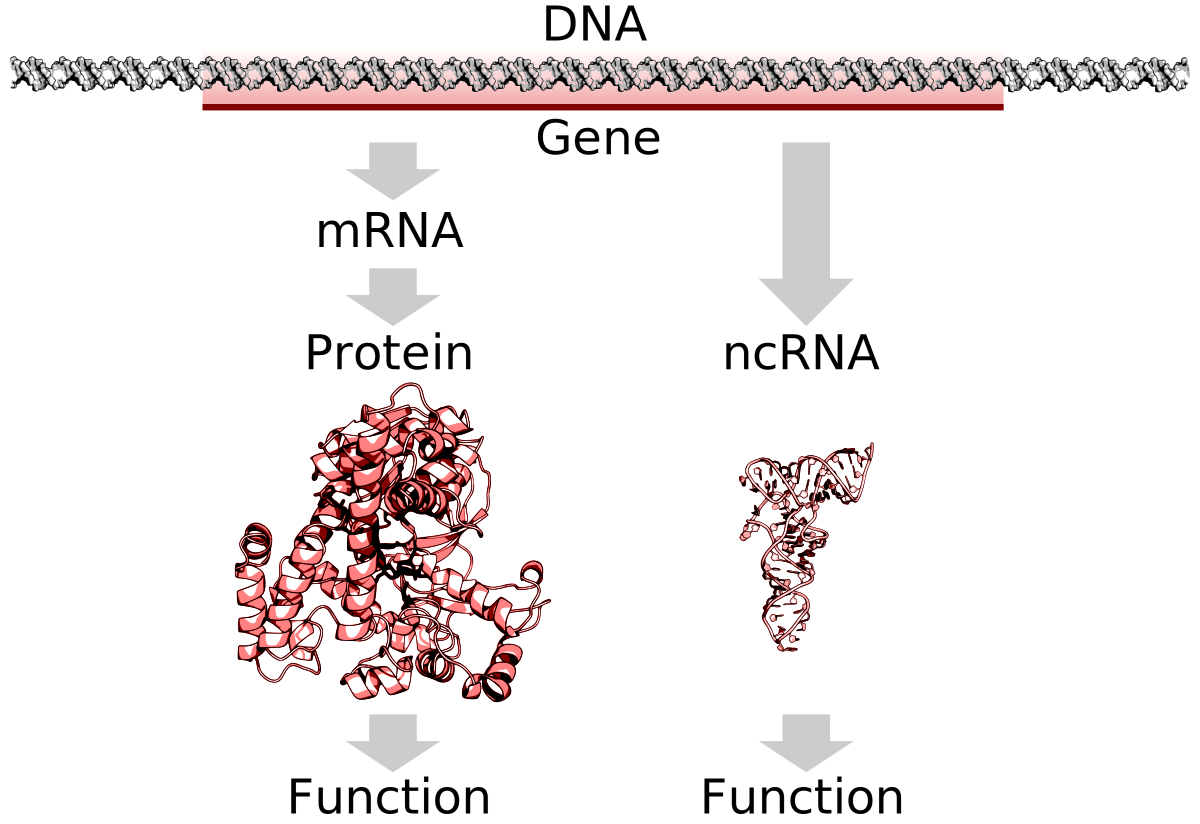
\includegraphics[width=0.5\linewidth]{./figs/gene} 

}

\caption{Central paradigm of biology: a gene, a specific region in the DNA, is first transcribed into RNA and then into proteins. Note, that for RNA-genes the RNA molecule is the end product itself, which is referred to as non-coding RNA (ncRNA) (Source: Thomas Shafee, Wikipedia)}\label{fig:centralParadigm}
\end{figure}

Figure \ref{fig:transcriptionTranslation} shows the process of transcription of a gene from DNA to RNA and the translation of RNA to proteins.

\begin{enumerate}
\def\labelenumi{\arabic{enumi}.}
\item
  The transcription of DNA to RNA is initiated by opening the
  DNA double strand. Then a complementary RNA strand is synthesized by exploiting that A hybridizes to U (or T) and G to C through hydrogen bounds.
\item
  Once that the complementary RNA strand is made, it is further processed in the nucleus into messenger RNA (mRNA). The mRNA travels from the cell nucleus to the cell cytosol (cell liquid) where it is translated into proteins, and, where the majority of the reactions take place.
\item
  There mRNA is translated into proteins by ribosomes.
  In the ribosomes the mRNA is bound to transfer RNA (tRNA). tRNA can bind to the mRNA molecule if it has 3 consecutive nucleotides that are complementary to the triplet of the 3 consecutive nucleotides on the mRNA template that is lying in the ribosome.
\item
  The transfer RNA transports one specific amino-acid that is then incorporated in the protein that is being formed, which is the growing amino acid chain in Figure \ref{fig:transcriptionTranslation}. The sequence of 3 consecutive nucleotides of DNA of a gene is therefore also called a \emph{codon} because it encodes for a specific amino acid.
\item
  Upon incorporation, the ribosome shifts to the next triplet of the mRNA and the next transfer RNA is bound to it, and so on until a stop codon is reached and the protein is finished.
\end{enumerate}



\begin{figure}

{\centering 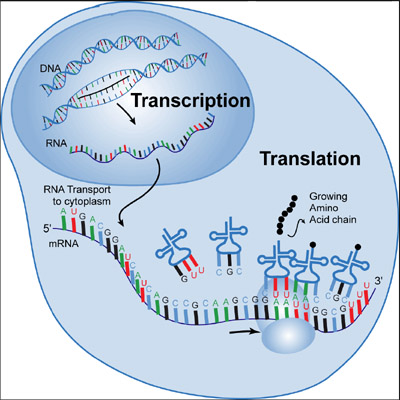
\includegraphics[width=0.5\linewidth]{./figs/transcription_2} 

}

\caption{In the cell nucleus the DNA strand opens up and is transcribed into an RNA molecule. Upon processing, the messenger RNA (mRNA) travels from the nucleus to the cytosol where it is translated into proteins. The mRNA is the template that fits into a ribosome that has the function to bind transfer RNA molecules to the mRNA template. It does that by hybridising to a tRNA, which has a triplet of three nucleotides that are complementary to those of the mRNA template. The tRNAs have a amino acid on their tail, which is incorporated into a long chain of amino acids, the protein that is produced. If the amino acid is incorporated, the ribosome moves to the next triplet and the process happens all over with a new tRNA (Source: \href{http://www.tokresource.org/tok_classes/biobiobio/biomenu/transcription_translation/}{tokresources.org})}\label{fig:transcriptionTranslation}
\end{figure}

There are in total 64=4\(^3\) codons encoding for each of the 20 amino acids, and, for a start and a stop codon to initiate and stop the protein translation, respectively. Hence, there is a redundancy in the code, see \ref{fig:codonTable}.

\begin{figure}

{\centering 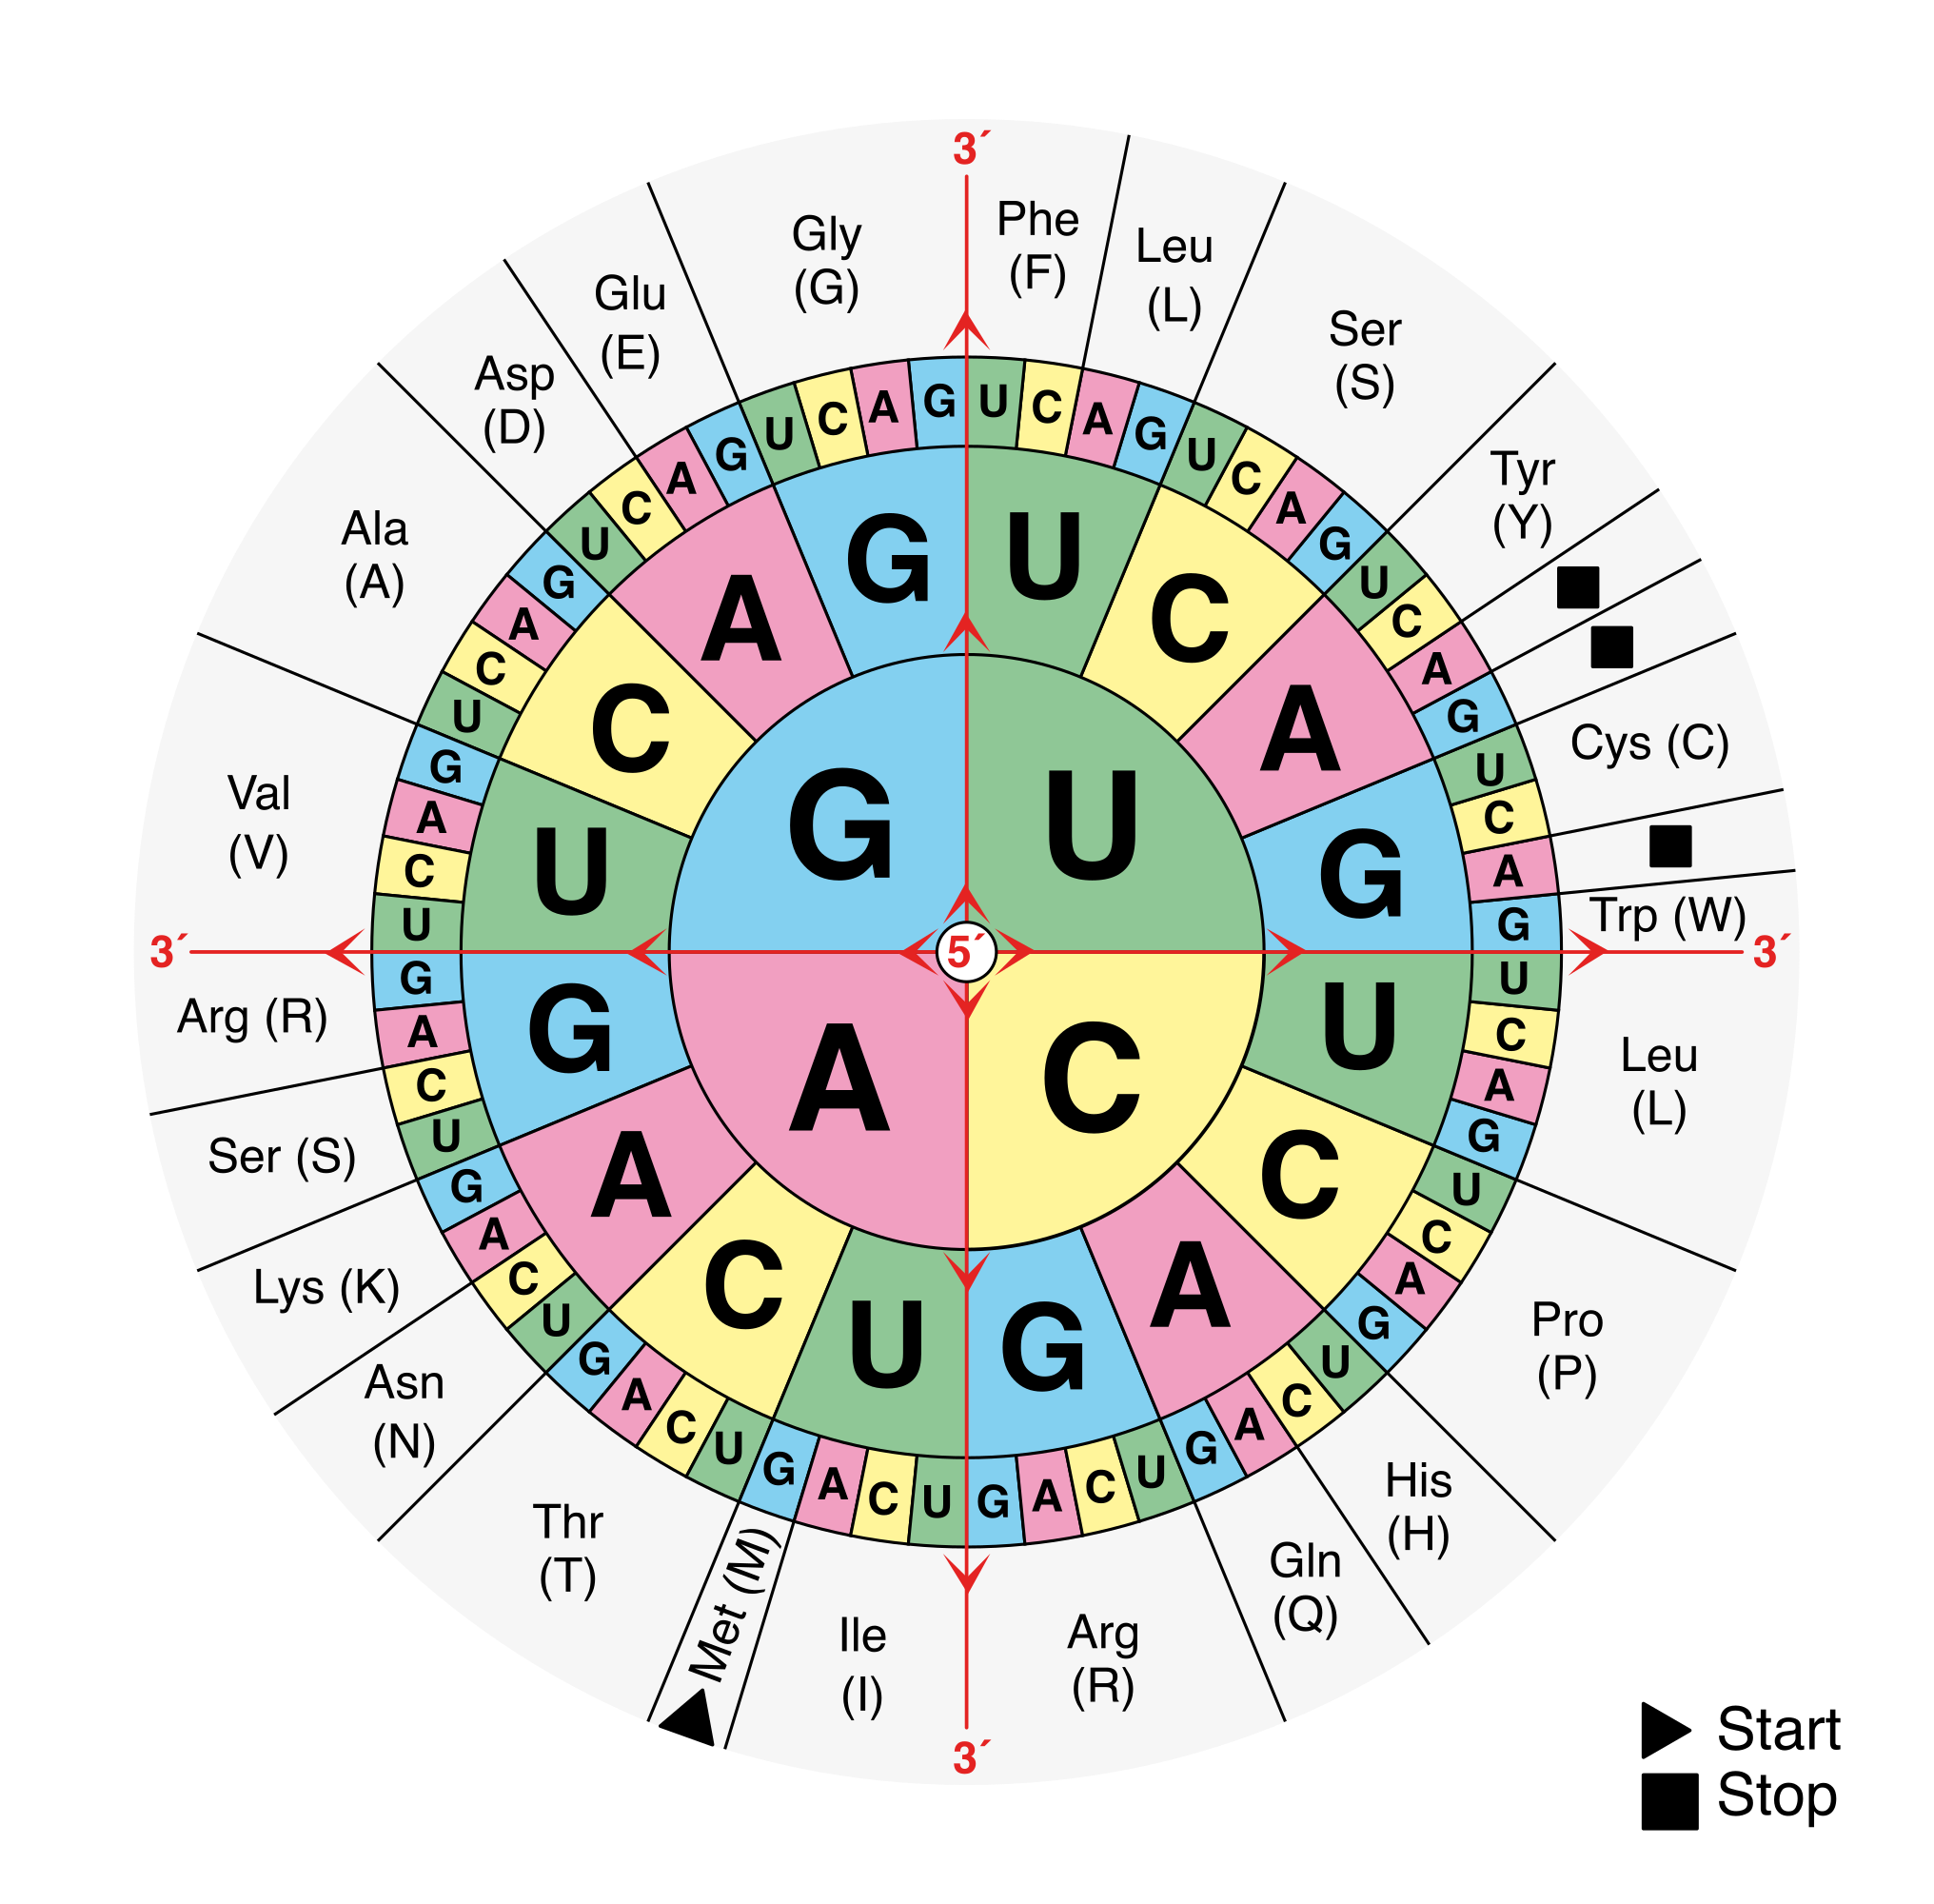
\includegraphics[width=0.5\linewidth]{./figs/Aminoacids_table} 

}

\caption{Codon table connecting triplets of nucleotids to amino acids (Source: Wikipedia)}\label{fig:codonTable}
\end{figure}

We can learn an important message from the codon table:

\begin{itemize}
\item
  There is no chemical necessity that explicitly connects the three nucleotides ``CGG'' to the amino acid arginine rather than to glutamine.
\item
  Nucleotides themselves do not seem to a have chemical connection to the amino acids they encode
\item
  Therefore we call it a code or information rather than just ``genetic chemistry''
\end{itemize}

The code apparently evolved so that many mutations give rise to

\begin{itemize}
\tightlist
\item
  synonymous codons (same amino acid) or
\item
  to incorporate amino acids that are similar
\end{itemize}

so that protein function is conserved.

DNA is thus the carrier of genetic information. However, RNA plays a more central role:

\begin{itemize}
\tightlist
\item
  Messenger RNA brings the genetic information from the cell nucleus to the cell cytosol where they are translated into proteins and where most of the chemical reactions take place.
\item
  Ribozymes, i.e.~catalytic RNA molecules, initiate and speed up particular reactions
\item
  Transfer RNA plays an crucial role in the translation of proteins
\item
  An RNA primer, i.e.~a small RNA molecule, is essential to copy DNA
\item
  RNA also acts as carrier of genetic information, e.g.~corona virus.
\end{itemize}

\newpage

\hypertarget{maturanaVarela}{%
\section{Maturana and Varela: a Systems View of Life}\label{maturanaVarela}}

In the reader of the Biodanza teacher training ``Module IV: Biological Aspects of Biodanza'' Rolando Toro also introduced the term \emph{autopoiesis}.

\citet{capraLuisi2014} write in their book ``The Systems View of Life'', that the ``term was coined by Varela and Maturana in the 1970s. \emph{Auto}, of course, means \emph{self} and refers to the autonomy of self-organising systems; and \emph{poiesis} (which shares the same Greek root as the word poetry) means \emph{making}. So, \emph{autopoiesis} means self-making''.

They continue stating that ``the main characteristic of life is self-maintenance due to internal networking of a chemical system that continuously reproduces itself within the boundary of its own making''.

Indeed, a living cell is the smallest autopoietic unit.
The cell consists of a complex internal network of chemical reactions and this within the boundary of its outer membrane.
It can organize itself, maintain itself, can make copies of itself and this with the enzymatic machinery that is present in the cell itself.

Networks of cells are then combined in larger autopoietic units, e.g.~

\begin{itemize}
\tightlist
\item
  our gut microbiome that consists of a network of billions of unicellular bacteria and yeasts from which unique metabolic functions emerge that are essential for digesting our food, or,
\item
  our tissues, networks of our own cells from which novel functions emerge, e.g.~our thinking that emerges from the complex network of neurons in our brain.
\end{itemize}

An organism or a biological system can therefore not be broken down or reduced to its parts to provide a complete understanding of it. A complete understanding is only possible when it is viewed as a whole.
Indeed, new functions emerge at a higher level from the network that has been formed between its lower-level parts. Varela refers to these properties with the term \emph{emergent properties}.

\hypertarget{emergent-properties}{%
\subsection{Emergent properties}\label{emergent-properties}}

Emergent properties can be found at each level. At the chemical level, where the protein hemoglobin for instance has the unique property that it can transport oxygen. This property emerges from its unique 3D structure (see Figure \ref{fig:hemoglobin}). We could never have derived its biological function at the protein-level by breaking it down to its constituting amino acids and only studying the individual properties of each of these amino acids (Note that amino acids are the biological building blocks of proteins).

\begin{figure}

{\centering 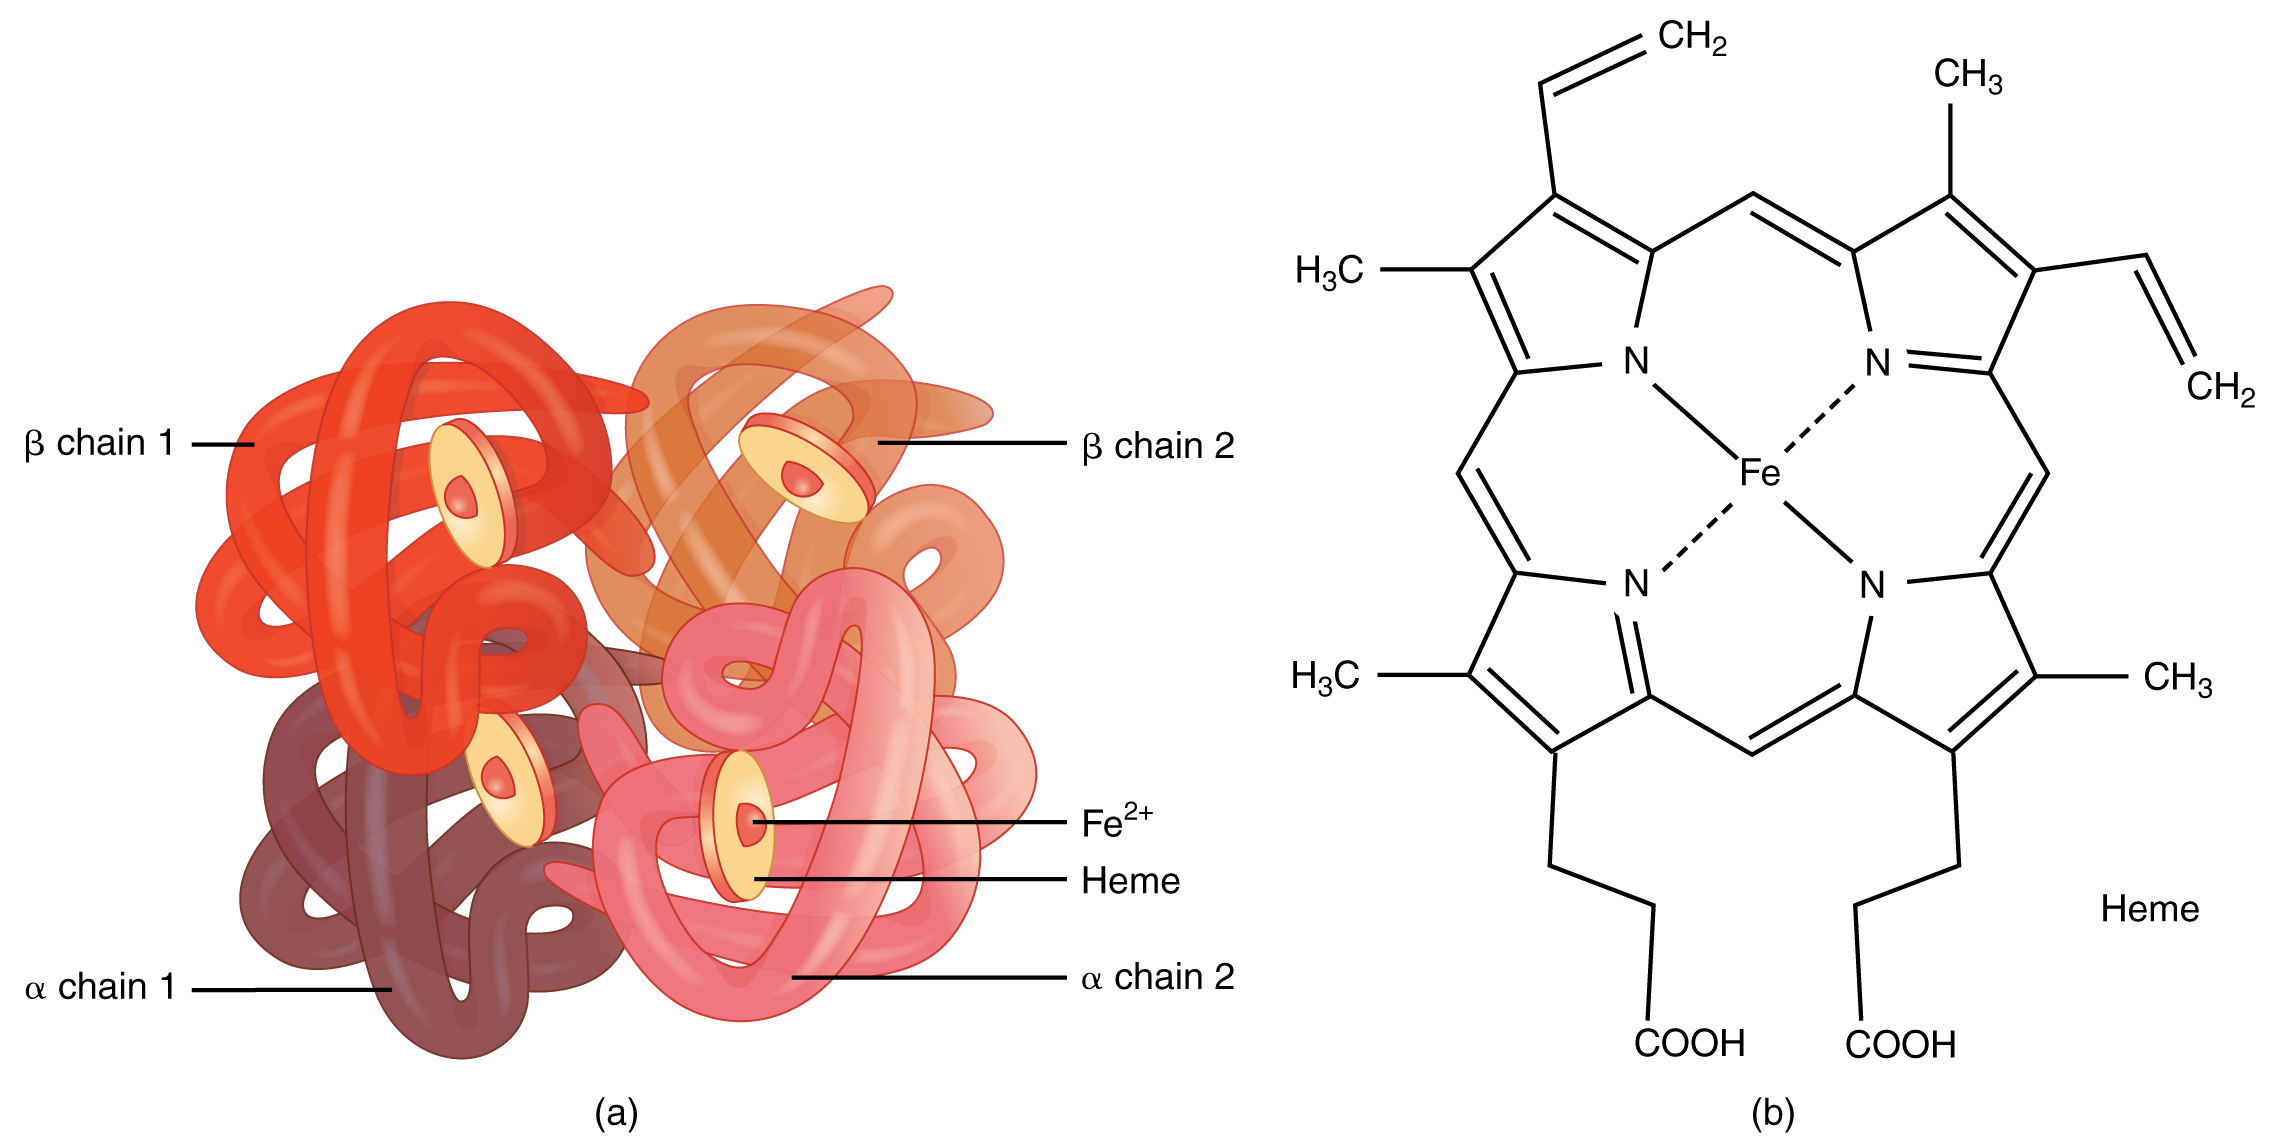
\includegraphics[width=1\linewidth]{./figs/hemoglobin} 

}

\caption{Structure of hemoglobin that consists of 4 subunits, each having a heme group with an iron molecule that can bind oxygen. This function emerges from its unique 3D structure (Source: Wikipedia)}\label{fig:hemoglobin}
\end{figure}

So hemoglobins' property to transport oxygen naturally emerges at the protein level upon combining many simple amino acid molecules in the appropriate sequence. Indeed, this specific long chain of amino acid spontaneously folds into a unique 3D structure that gives the hemoglobin protein its unique function.

Lichens are another compelling example of emergent properties (Figure \ref{fig:lichen}). Lichens are true colonists. They were among the first organisms that colonized the earth surface.
Indeed, when glaciers pull back lichens appear on the bare hostile rocks and in the course of thousands of years they can convert these rocks into soil, an environment that is fertile for other species. However, their unique and important properties for life on earth could never have been expected when only studying a lichen's components.

\begin{figure}

{\centering 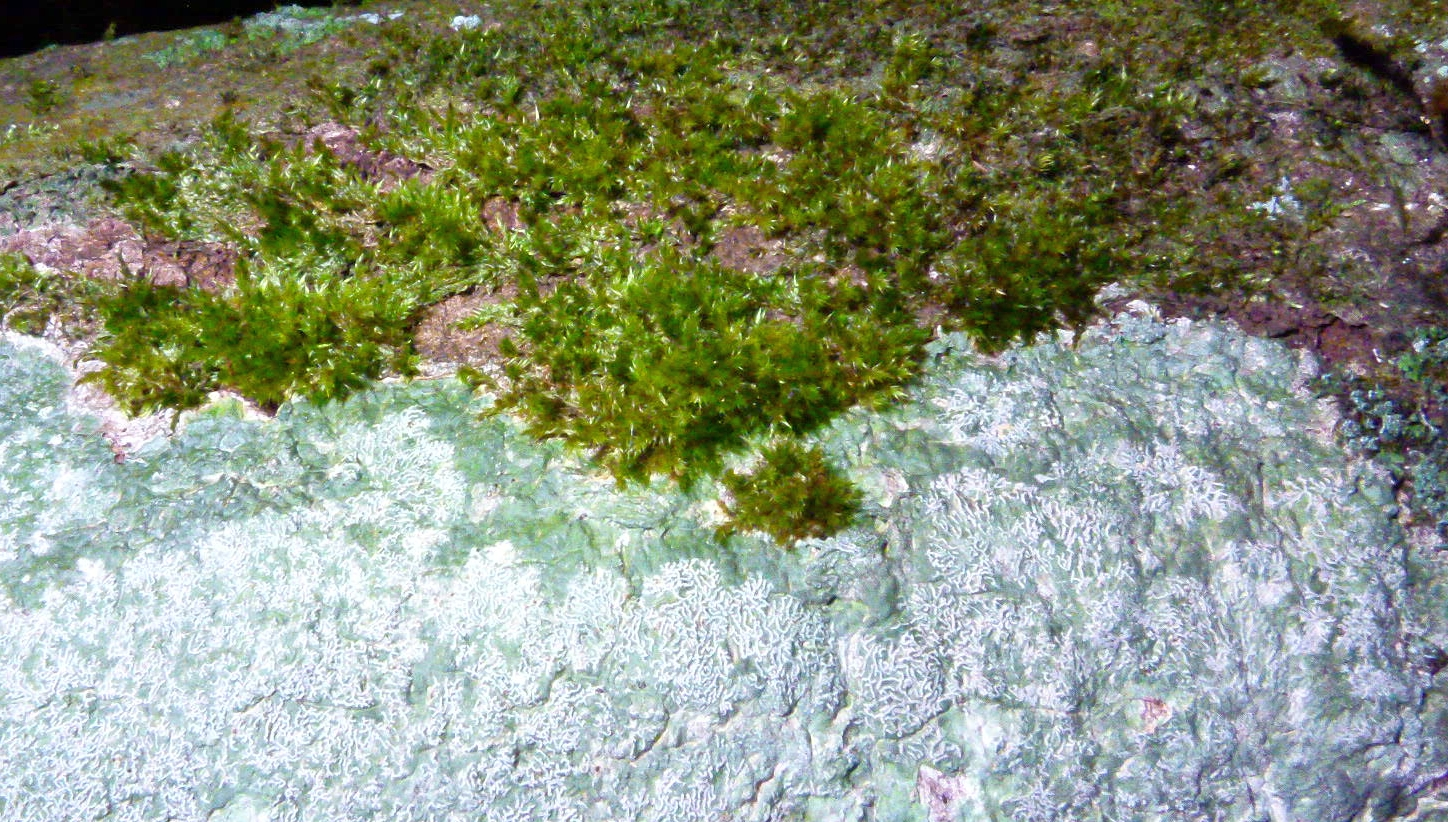
\includegraphics[width=0.45\linewidth]{./figs/lichen} 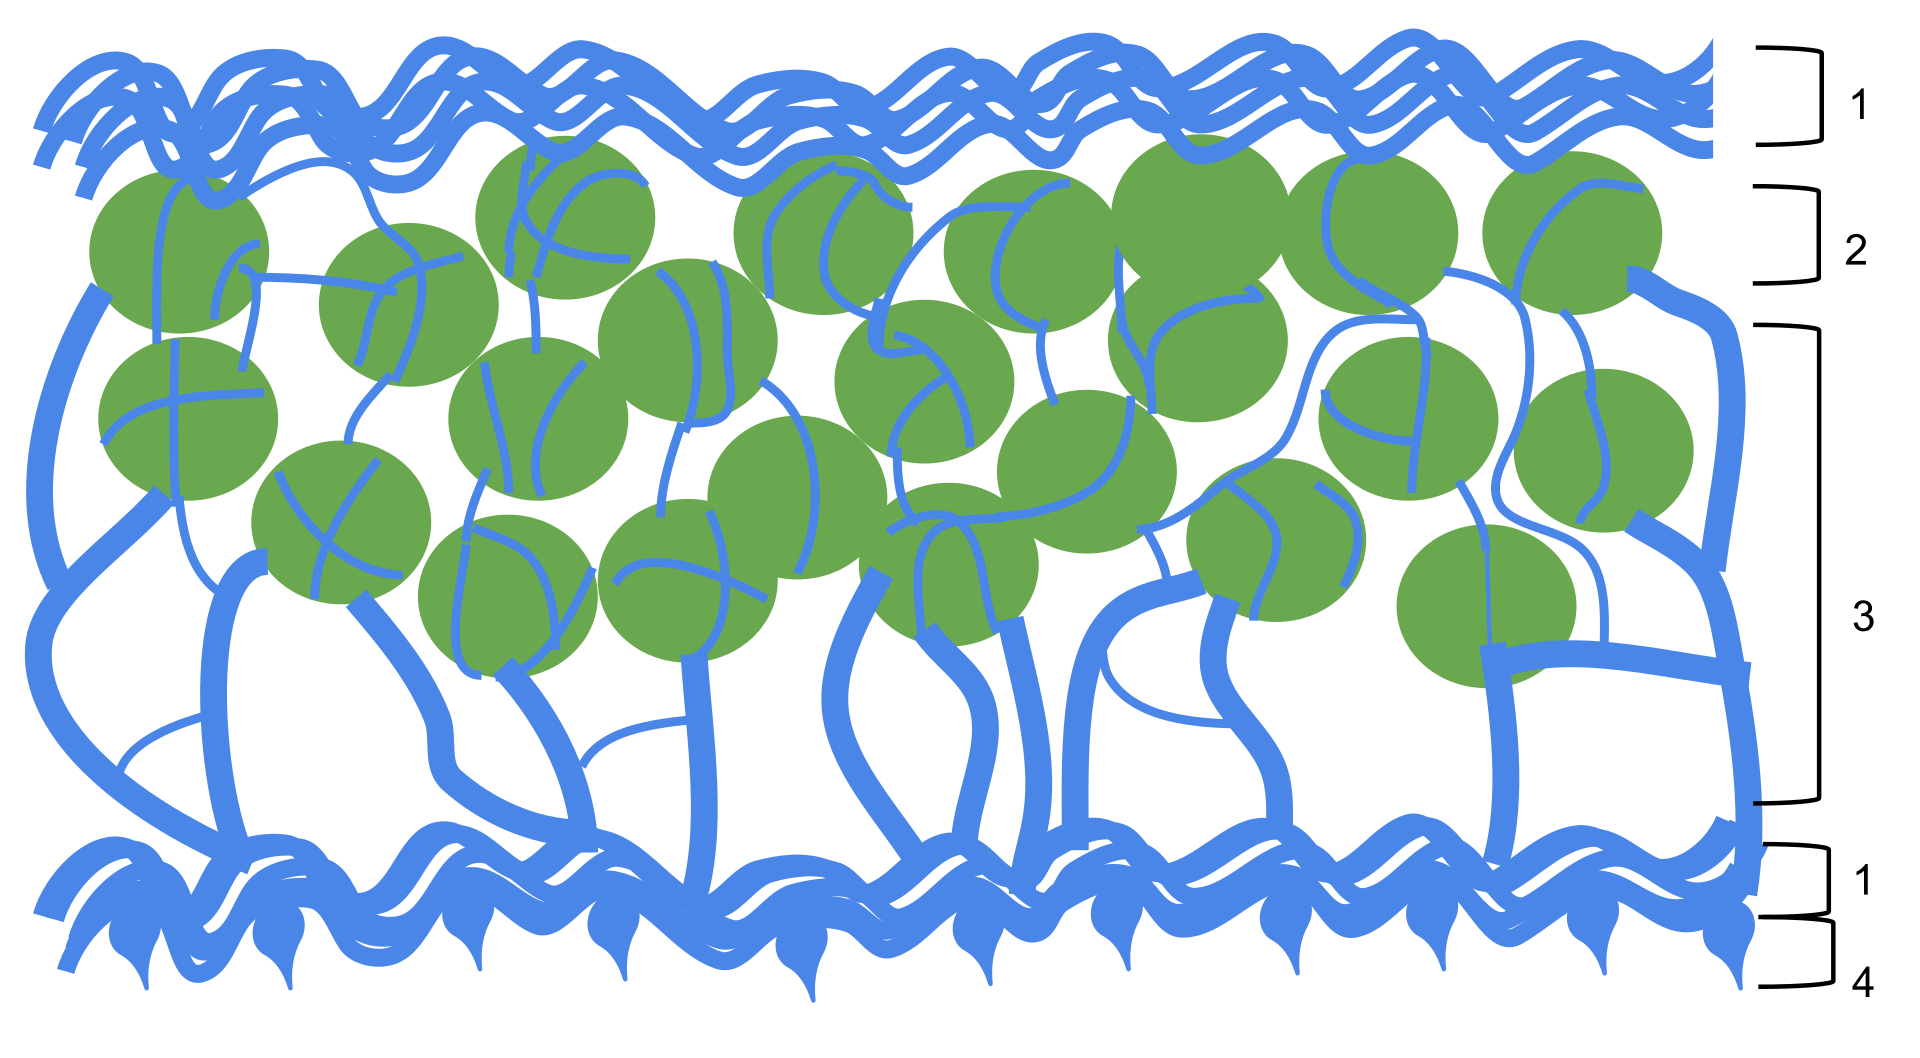
\includegraphics[width=0.45\linewidth]{./figs/LichenDiagram} 

}

\caption{Lichens. Left: Lichens, a unique organism that can colonize rocks (Source: Shyamal, Wikipedia). Right: Lichens are a symbiosis of a green alga and a fungus. 1. Thick layers of fungal hyphae protecting the green alga 2. Green algae 3. Loosely packed fungal hyphae 4. Anchoring fungal hyphae that act as a kind of roots (Jdurant, Wikipedia).}\label{fig:lichen}
\end{figure}

Although lichens macroscopically look like one being, they are effectively two beings: a green algae with the precious gift of photosynthesis that turns sunlight and air into sugars, and, a fungus that provides shelter and is gifted with the art to mine the rocks for minerals, but which cannot make sugars. They are joined in a symbiosis that is so close that their union becomes an entirely new organism. When biologists tried to unravel this unique algal-fungal marriage, they started to grow them in the lab in ideal conditions for both algae and fungus. However, under these conditions they both happily lived next to each other. So the unique properties of lichens could not be delineated from studying both species apart. Only when the scientists exposed them to ecofactors that became so harsh, they teamed up in reciprocity and gained their unique transformative power of turning rocks into fertile environments \citep{Kimmerer2013}.

\hypertarget{life-as-an-emergent-property}{%
\subsection{Life as an emergent property}\label{life-as-an-emergent-property}}

\citet{capraLuisi2014} convincingly argue that the same holds at any level and for life itself. Indeed the autopoietic property of a cell originates by properly combining all its molecules in the large networks of chemical reactions from which its structure and organisation, self maintenance, and self replication emerge. We cannot localize life. Life is simply a global property that emerges from the collective interactions of all kind of molecules in a cell, of the collection of cells in a tissue, of the collection of tissues in a organ system, of the collection of organ systems for an organism, of the collection of organisms in a population etc.
At each level we have a network of lower level components from which new properties naturally emerge.

So life itself is an emergent property, it is not present in the parts it originates from, and only emerges when its parts are assembled together correctly.

\hypertarget{life-as-a-gestalt-of-autopoetic-unit-cognition-and-environment}{%
\subsection{Life as a gestalt of autopoetic unit, cognition and environment}\label{life-as-a-gestalt-of-autopoetic-unit-cognition-and-environment}}

For Maturana and Varela cognition is also inseparable from autopoiesis \citep{capraLuisi2014}. Each living organism is an open system that interacts with its environment through its sensory arsenal. It senses its environment, it feeds on its environment, releases products in it, it changes its environment, and, actualizes itself to its environment. The fact that an organism is changing its environment is often overlooked. However, life has dramatically transformed Earth. Indeed, think of photosynthesis for instance that radically changed Earth by the release of the highly reactive molecule oxygen.

An organism at any time in its development is a record of its previous interactions with its environment and that determines its future interactions.
Hence, cognition is a natural product of its evolution.

Varela sees life as a gestalt of three domains \citep{capraLuisi2014}:

\begin{itemize}
\tightlist
\item
  Environment,
\item
  Cognition and
\item
  The autopoietic unit.
\end{itemize}

Life is the synergy of these three domains, which he refers to as the embodied mind.

\hypertarget{our-social-system-as-an-emergent-property}{%
\subsection{Our social system as an emergent property}\label{our-social-system-as-an-emergent-property}}

The insights of Maturana and Varela have the compelling implication that we no longer need the duality of matter and soul when trying to understand life. Life naturally arises as an emerging property of the large networks of matter or molecules at the level of each individual cell, the basic autopoietic unit, and then new properties emerge at a higher level when combining autopoietic units into tissues, organs, organ systems, organisms, populations, etc.

As such, we can also view our cognitive awareness as an emerging property of the network of our neurons in our brain in response to the history of our interactions with our environment. Indeed, consciousness is an expression of life, it is embodied and pathologies can arise when mental processes dissociate from our bodily experiences. Our embodied mind is indeed remarkable. However, in our arrogance we are often blind for the intelligence that emerges in other forms of life. Nevertheless, similar to other species, the unique novel functions and processes that do arise when human entities are forming networks are astounding.

Indeed, at the next level, the network of people, our rich psycho-socio-emotional realm emerges. As human beings, our lives do not only take place in the physical domain, but also in the symbolic social domain, which is also very important for our development. Hence, our behavior in the physical domain is shaped by the ``laws of nature'', while our behavior in the social domain is governed by rules that are generated by the social system itself \citep{capraLuisi2014}. Moreover, research in the social sciences has pointed out that social networks exhibit the same general principles as biological networks. So, as human beings we develop ourselves in an organised ensemble with internal rules that are generated by the networks and their boundaries, i.e.~the physical boundary in our biological networks and the cultural boundary in our social networks \citep{capraLuisi2014}.

\hypertarget{shared-bio-logic-from-cell-to-social-system}{%
\subsection{Shared ``bio-logic'' from cell to social system}\label{shared-bio-logic-from-cell-to-social-system}}

Similar to the biochemical system of a cell, the social system is an open system with social feedback loops. Indeed, each social system needs to sustain itself in a stable but dynamic way, by letting new members, materials and ideas to enter the system, which will in turn be transformed by the internal rules or organisation of the system \citep{capraLuisi2014}, leading to a kind of ``social homeostasis''. Sometimes, these novel ideas can be so powerful that they transform the social system by itself, i.e.~switching it towards a novel attractor. At the individual level, however, the transformation implied by the social system sometimes are a bliss, but they also can cause trauma. The observation that the ``bio-logic'' or pattern of organisation of a simple cell is similar to that of an entire social structure has large implications.

Indeed, as \citet{Kimmerer2013} points out so convincingly in her book Braiding Sweetgrass, these insights also invites us to learn from all forms of life that are surrounding us.
The lichen example can teach us on our relationships and society. Indeed, in the lab environment when resources were plentiful both the fungus and green algae did not interact, only when the environment became harsh for both of them, they join forces and take their unique lichen form where there are intimately intertwined. A similar disruption of our social function can be seen in our modern western society that is flooded by resources, which cultivates individualism and loneliness.

So this shared bio-logic from cells up to our symbolic realm, suggests a fundamental unity of life \citep{capraLuisi2014}, and that studying human development thus requires a unifying perspective, which Rolando Toro deeply embraced when he developed his system of Biodanza.

This bio-psycho-socio-emotional angle, although extremely interesting, is beyond the scope of this monograph as it can give food of thought for an entire monograph on itself.

\hypertarget{links-to-vital-unconciousness}{%
\section{Links to Vital Unconciousness}\label{links-to-vital-unconciousness}}

``Life is One'', all species originated from the same population of ancestral cells, they use the same chemistry, and the same encoding system to store their genetic information.
The wealth of living species, all with their own sensory arsenal, have all been shaped from our last universal common ancestor through evolution by interactions with their environment.
So we can feel that all living beings are intimately connected. Moreover, the emergent properties of networks of living beings follow the same ``bio-logic'' and suggest a fundamental unity of life.

The cells of living organisms act on internal and external stimuli by producing biochemical molecules, proteins, hormones, neurotransmitters, which in term shape their response and how they interact in their population.
Our response on ecofactors in the environment is largely determined by our embodied mind. This embodied mind emerged from the different levels of autopoietic units of which our organism consists together with the history of the interactions with the environment and social networks that we had ourselves, that our ancestors had and that the species had from which we evolved.

This intimate connection to life that is one, through our embodied mind, is in my opinion what Rolando was referring to with the term \emph{vital unconsciousness}.

So it becomes clear that all beings are sharing a kind of common cognition and this from ecosystem, population, organism, tissue, down to the cellular level. The latter, which Rolando also referred to as a kind of \emph{cellular psychism}: with a memory, and an ability for affinity, repulsion, solidarity and communication as well as recognition of similar autopoietic structures in other forms of life.

So this shared \emph{psychism} or \emph{vital unconsciousness} encompasses the origin of our instincts, bodily sensations and deeper knowledge that we can experience immediately from our embodied mind. Vivencia is a path to deeply connect, ameliorate and heal the vital unconsciousness, and, this along the five lines of Biodanza.

Now that we developed a basic understanding of important insights that shaped Rolando Toro's view on life, we will elaborate in the remaining chapters of this monograph on where, how and why biological aspects appear in the Model of Biodanza. Do note, however, that many of the concepts that we will touch upon from a biological perspective also have an important sociological, psychological, emotional and mystic dimension as a very substantial part of our human life takes place in the symbolic social domain.

\hypertarget{principles-of-cosmic-life-and-the-genesis-of-life}{%
\chapter{Principles of Cosmic Life and the Genesis of Life}\label{principles-of-cosmic-life-and-the-genesis-of-life}}

The biological aspects are the vertical axis of the Model of Biodanza.
At the bottom of the model, we first encounter the Principles of Cosmic Life and the Genesis of Life, which are indicate with the red box in Figure \ref{fig:modelCosmic}.

\begin{figure}

{\centering 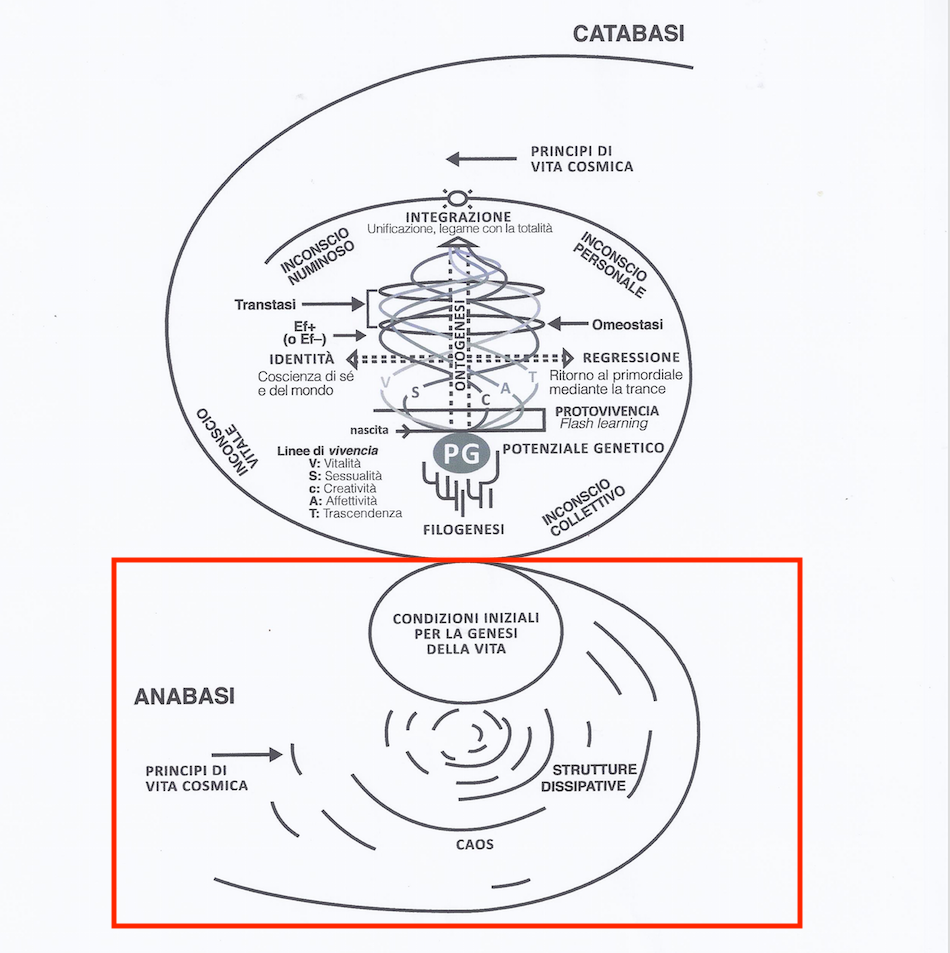
\includegraphics[width=0.5\linewidth]{./figs/biologischeAspectenBiodanzaDeelI} 

}

\caption{Model of Biodanza and Principles of Cosmic Life and the Genesis of Life}\label{fig:modelCosmic}
\end{figure}

We will start with the genesis of the universe and we conclude with the genesis of life. These two sections cover the concepts in the reader for module IV Biological aspects of Biodanza on these topics.

\hypertarget{genesis-of-universe}{%
\section{Genesis of Universe}\label{genesis-of-universe}}

An overview of the evolution of our universe is given in Figure \ref{fig:evolutionUniverse}.

\begin{figure}

{\centering 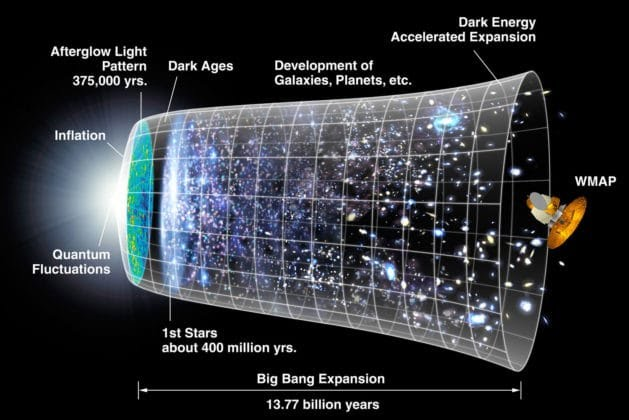
\includegraphics[width=1\linewidth]{./figs/originKosmos} 

}

\caption{Genesis and Evolution of our Universe (Source: NASA/WMAP Science Team, Wikipedia)}\label{fig:evolutionUniverse}
\end{figure}

The most common theory is that our cosmos started with the Big Bang.
A very energy-rich state.

By expanding the universe quickly cooled down enough for energy to be converted into mass, i.e.~the majority in hydrogen and a fraction in more heavy helium nuclei.

\hypertarget{genesis-of-stars}{%
\subsection{Genesis of Stars}\label{genesis-of-stars}}

Under the influence of the gravitational force, matter then started to cluster in nebula, gaseous clouds essentially consisting of hydrogen (H) and helium (He).

Due to concentration difference in these first nebula, these clouds further contracted and eventually imploded (See Figure \ref{fig:genesisStar}).

\begin{figure}

{\centering 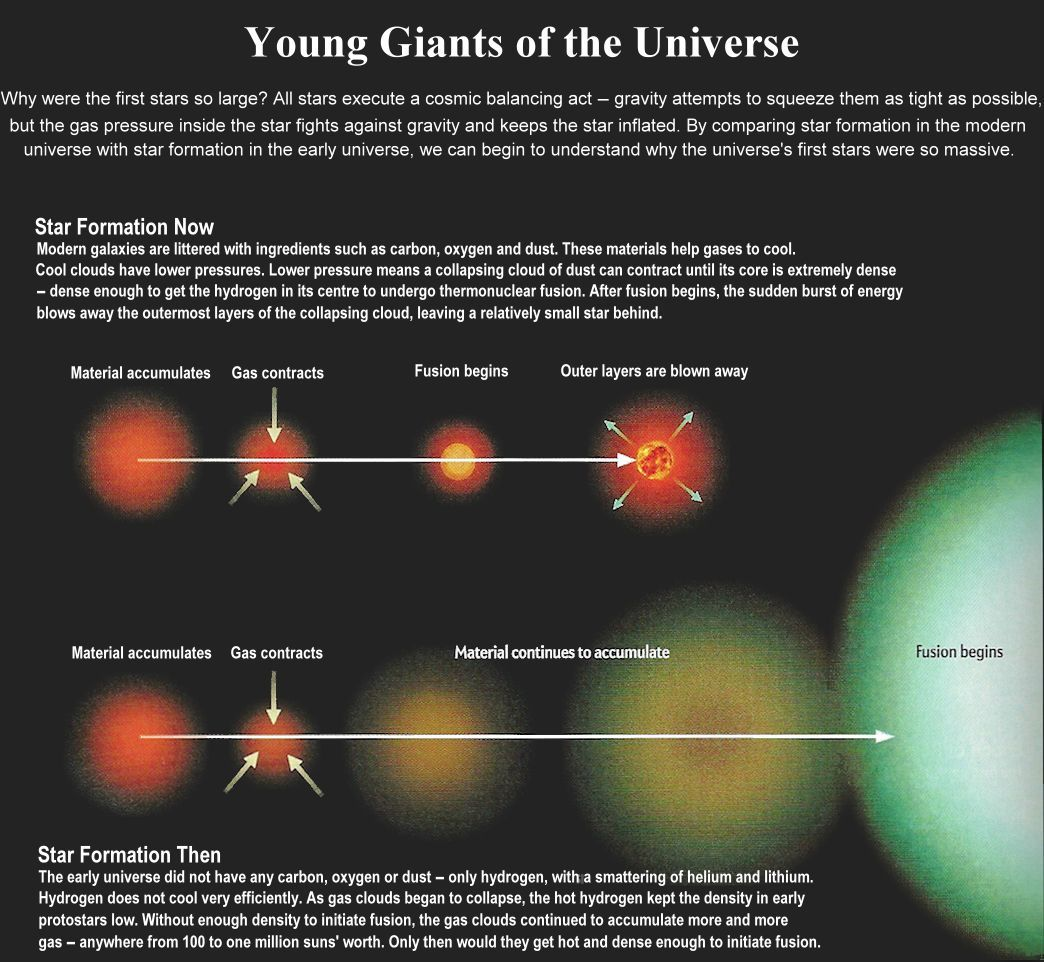
\includegraphics[width=1\linewidth]{./figs/I08-13-firststars6} 

}

\caption{Genesis of the first stars (Source: universe-review.ca)}\label{fig:genesisStar}
\end{figure}

Extreme heating in the nebula that imploded by gravity gave rise to a condition in which all matter was in the form of a super hot plasma.
In such a plasma nuclear fusion spontaneously takes place. In this process light atoms are combined into more heavy atoms and much energy is released.

First all hydrogen atoms are converted into helium (see Figure \ref{fig:nuclearFusion}). The mass of the resulting Helium nuclei is slightly lower than that of the original helium nuclei and the mass difference has been converted again into energy.

\begin{figure}

{\centering 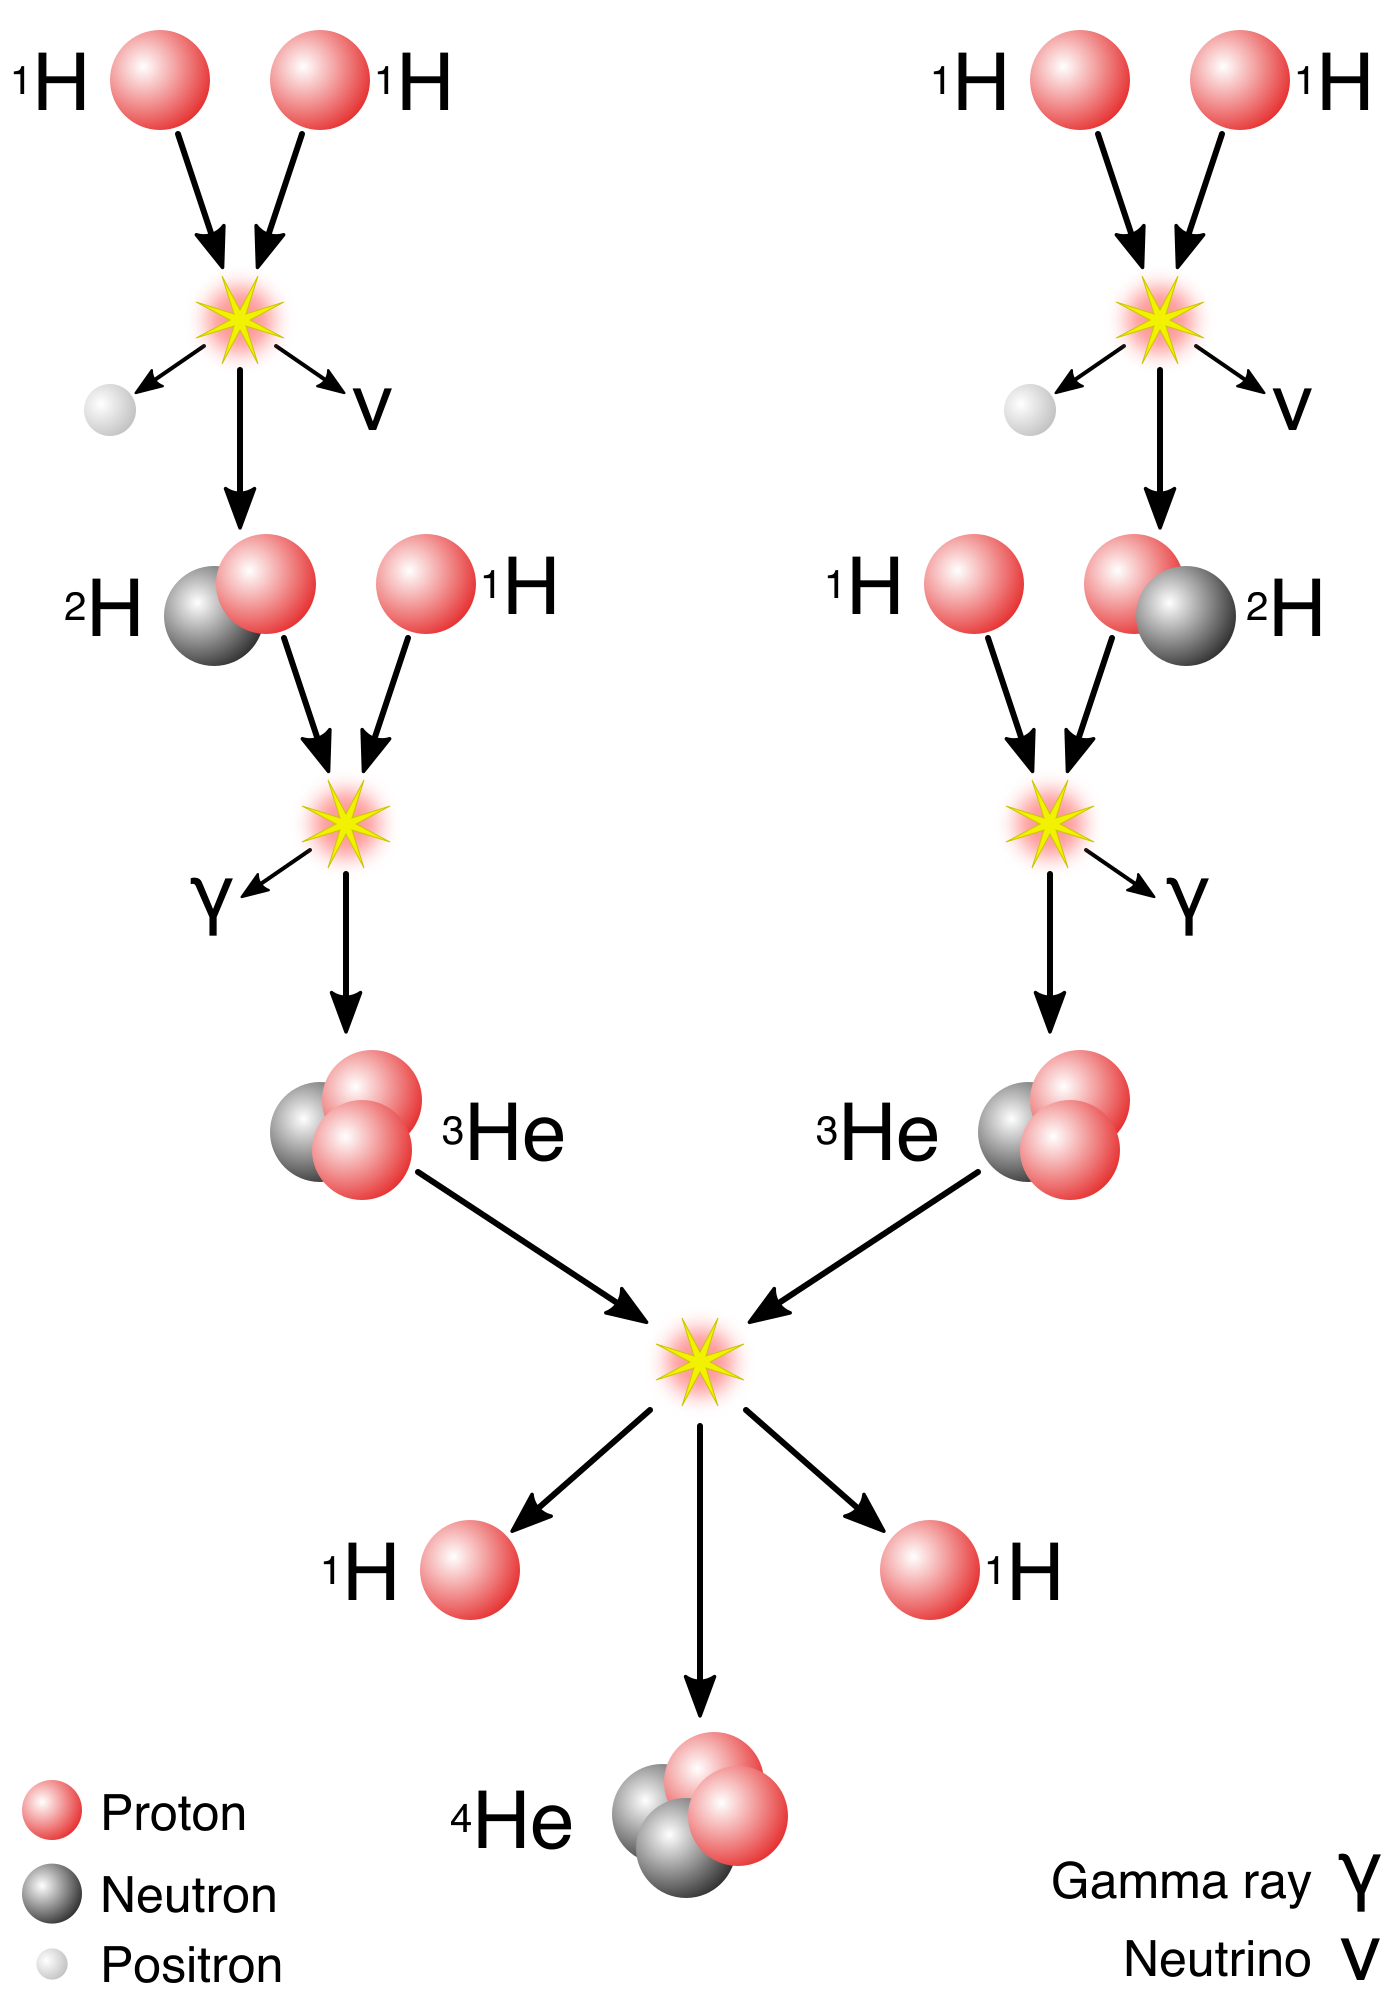
\includegraphics[width=0.5\linewidth]{./figs/fusion} 

}

\caption{Nuclear Fusion of hydrogen to the more heavy helium (Source: Sarang, Wikipedia)}\label{fig:nuclearFusion}
\end{figure}

If all hydrogen in a star is used, the fusion stops because the activation energy to convert helium to lithium is too high (Figure \ref{fig:fusionEnergy}).

\begin{figure}

{\centering 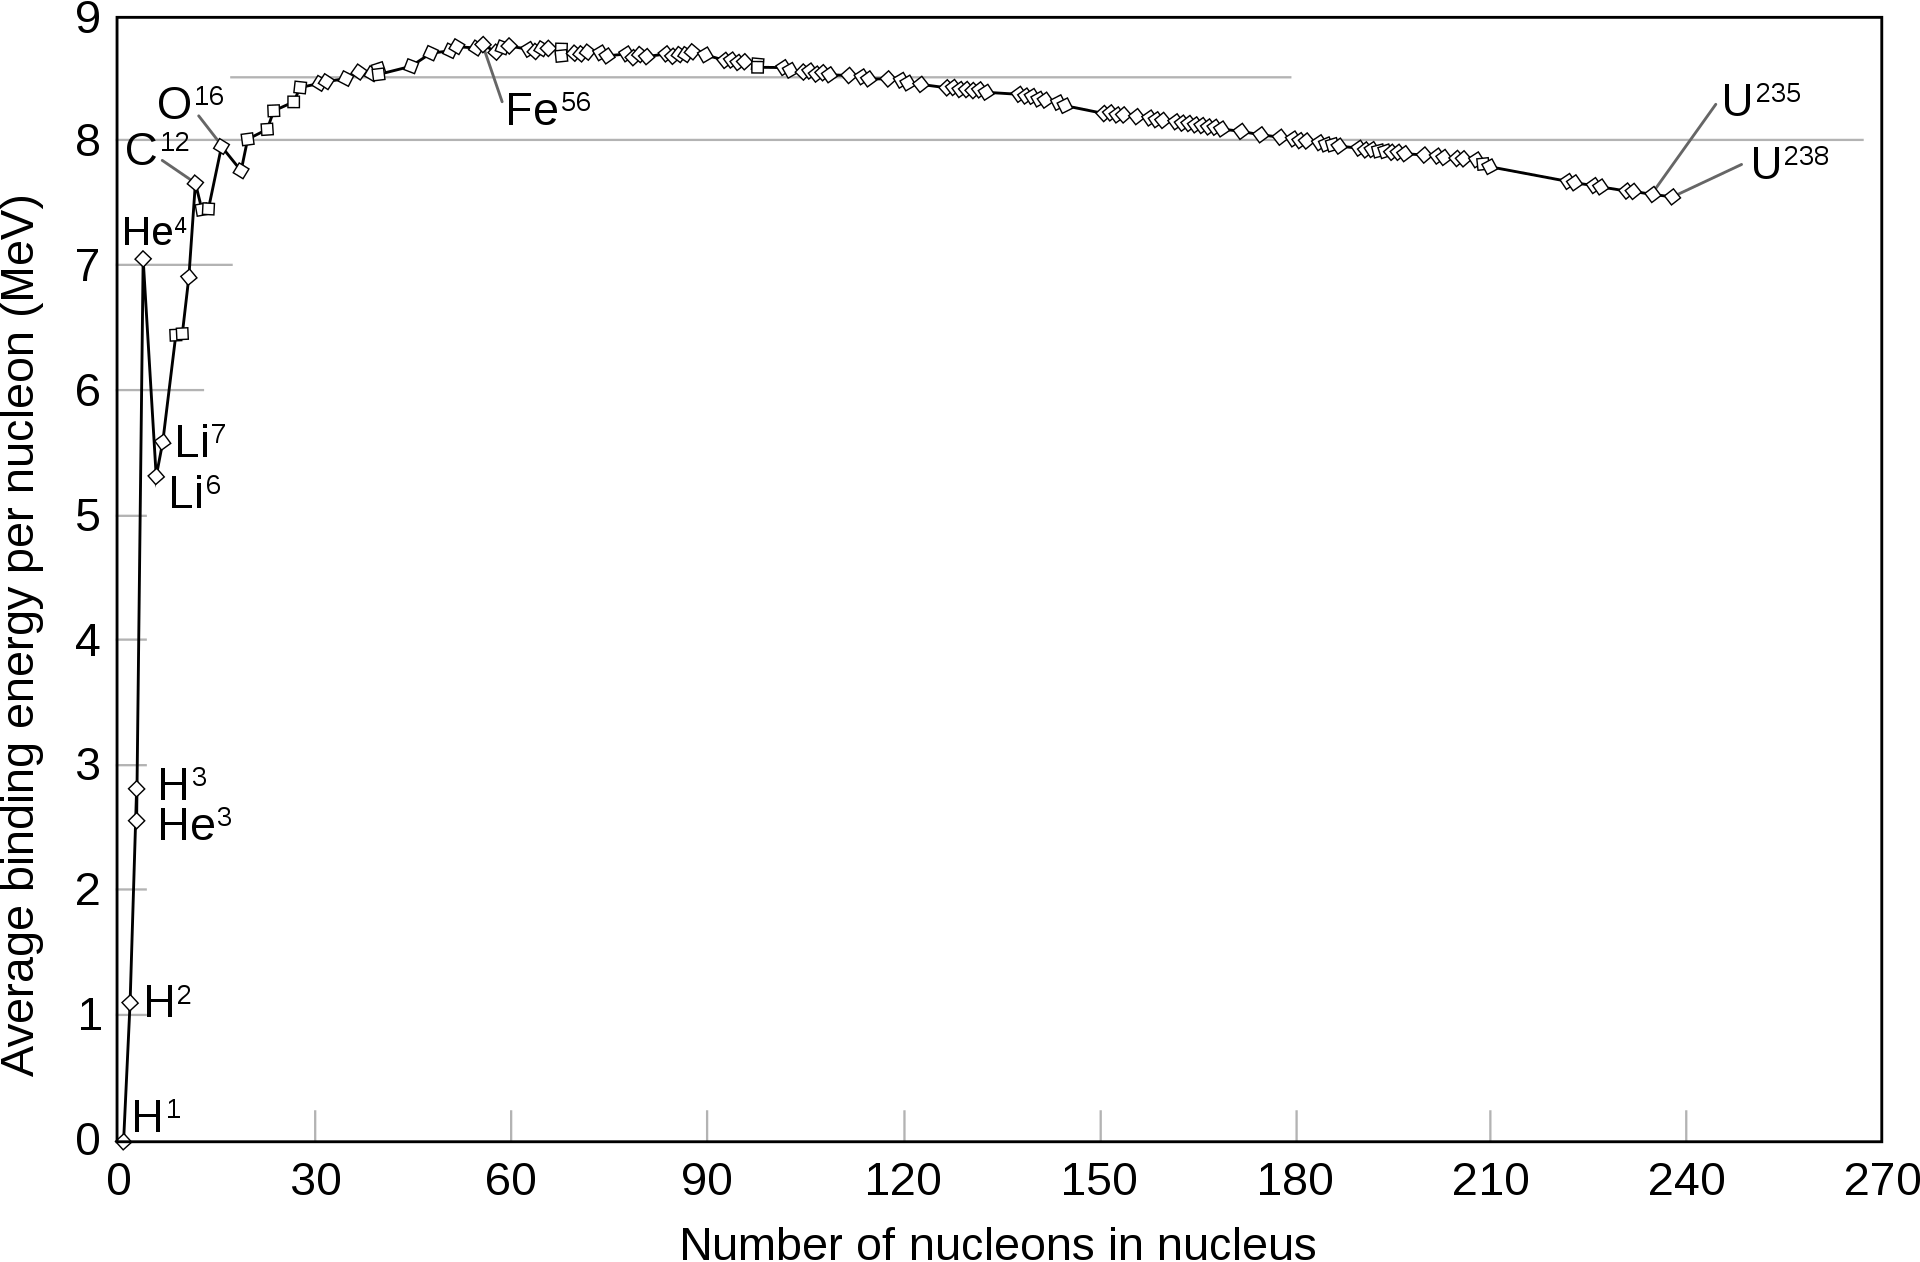
\includegraphics[width=0.5\linewidth]{./figs/fusionEnergy} 

}

\caption{Energy liberated by nuclear fusion. In a star nuclear fusion happens until Iron (Source: Wikipedia)}\label{fig:fusionEnergy}
\end{figure}

Therefore, the star cools down, implodes and subsequently explodes into a supernova (see Figure \ref{fig:supernova}). During the supernova nuclear fusion further occurs towards more heavy elements up to iron (Figure \ref{fig:fusionEnergy}) and these elements are projected in the universe.

\begin{figure}

{\centering 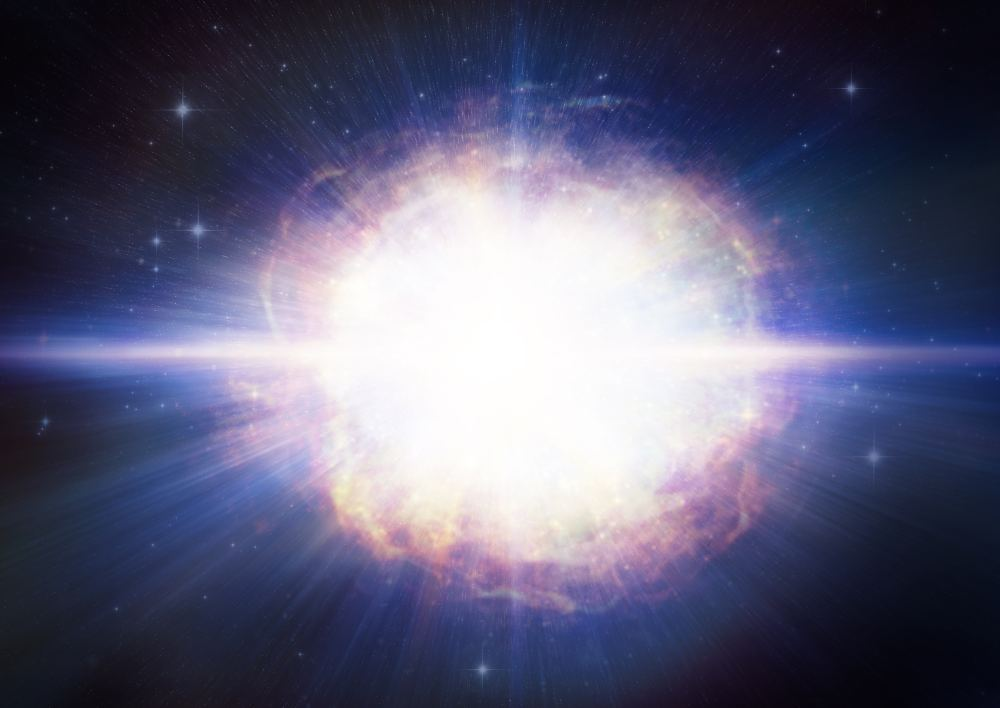
\includegraphics[width=0.5\linewidth]{./figs/hires} 

}

\caption{Supernova of a star (Source:  www.universetoday.com)}\label{fig:supernova}
\end{figure}

A supernova gives rise to new nebula and these will eventually lead to new stars and the whole process begins all over.

Hence, through nuclear fusion in the stars the more heavy atoms have been generated of which the bio-molecules of life are eventually built. So we are built out of cosmic dust!

\newpage

\hypertarget{carbohydrates-in-interstellar-space}{%
\subsection{Carbohydrates in Interstellar Space}\label{carbohydrates-in-interstellar-space}}

Upon nuclear fusion in the stars many different elements are formed. For life, hydrogen, carbon, oxygen, sulfur, phosphorous and nitrogen atoms, among others, are key to compose organic matter.

In interstellar space, carbon reacts spontaneously with other elements to form poly-aromatic carbohydrates (PAHs). This is for instance visible in a photograph of the Cat's paw nebula (Figure \ref{fig:catPawNebula}). In the green regions radiation of hot stars induces fluorescence of PAHs.

\begin{figure}

{\centering 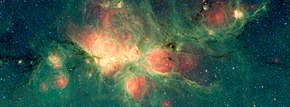
\includegraphics[width=0.5\linewidth]{./figs/orionWithPAH} 

}

\caption{Cat's Paw nebula, in the green regions radiation of hot stars induces fluorescence of PAHs (Source: NASA/JPL-Caltech, Wikipedia)}\label{fig:catPawNebula}
\end{figure}

PAHs were already be generated shortly after the Big Bang. Once they are produced, they are further transformed in interstellar space upon reaction with hydrogen and oxygen among others to form precursor molecules (``forerunners'') for amino acids and nucleotides, which are the building blocks of proteins, and, of RNA and DNA, respectively. So these simple building blocks that are essential for the chemistry of life are already omnipresent in space.

This, among other arguments, let Christian de Duve to formulate his quote that ``Life is an obligatory manifestation of matter, written into the fabric of the universe'' \citep{deDuve2002}.

\hypertarget{genesis-of-life}{%
\section{Genesis of Life}\label{genesis-of-life}}

In a remote corner of our milky way, which is an average galaxy, an average planet was formed, which we know as our planet Earth.
After the Earth cooled down liquid water was formed. The unique features of liquid water are essential for life as we know it.
Indeed, once liquid water was available, life emerged in less than 300 million years, which is very short time interval on the geological timescale.

So on earth conditions emerged that made the \emph{``genesis of life''} as we know it, possible. The exact process that led to the life forms on earth is unknown and will probably remain so.
However, a general rationale is displayed in Figure \ref{fig:originOfLife}.

\begin{figure}

{\centering 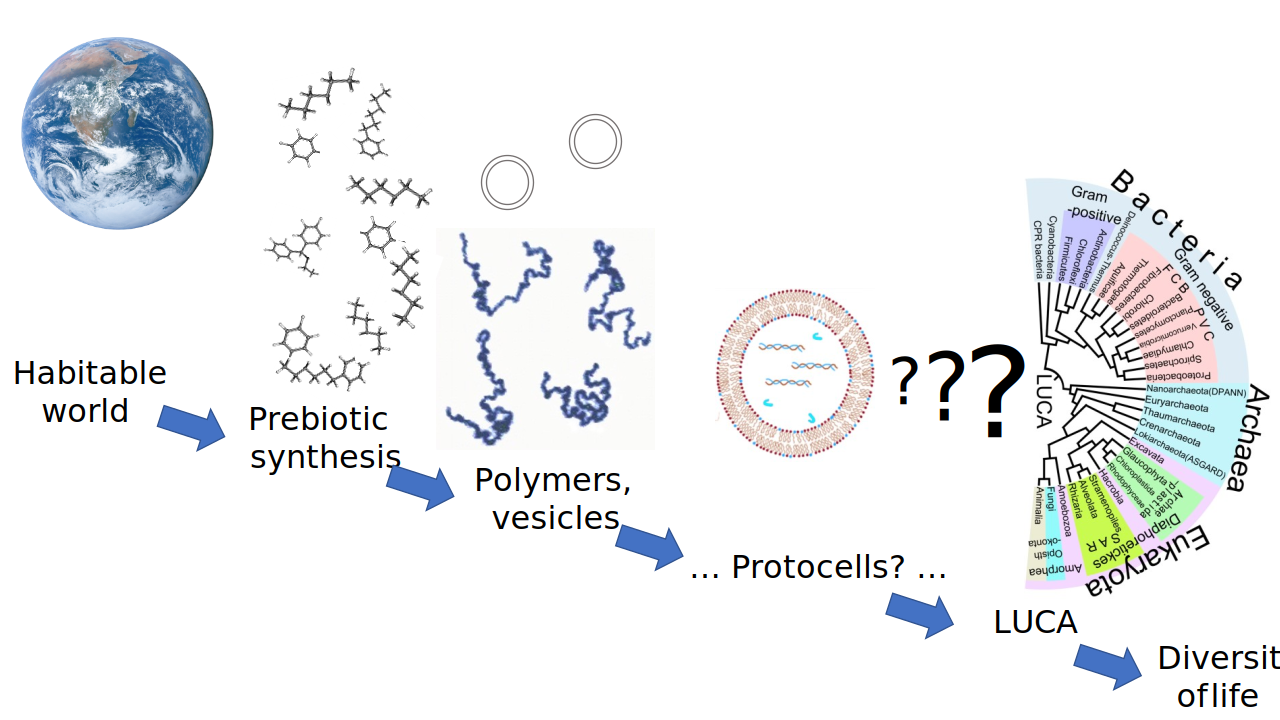
\includegraphics[width=1\linewidth]{./figs/origin_of_life_stages} 

}

\caption{Stages in the origin of life range from well-understood, such as the abiotic synthesis of simple organic molecules, to largely unknown, like the origin of the last universal common ancestor (LUCA) with its complex molecular functionalities. (Source: Chiswick Chap, Wikipedia)}\label{fig:originOfLife}
\end{figure}

First, a chemical evolutionary process gave rise to organic molecules with increasing complexity. It is a general consensus that RNA molecules emerged first from free nucleotides. RNA molecules are known to be catalytic and are carriers of genetic information. They can also replicate themselves under anoxic conditions (in the absence of oxygen) and in the presence of iron, conditions that occurred at young planet Earth (e.g. \citet{Williams2013}). These RNA molecules evolved either alone, the RNA-world hypothesis, or already in conjunction with proteins.

Next, it is assumed that prebiotic molecules, which could self-replicate, were encapsulated by phospholipids, which spontaneously form membrane like structures. This resulted in a protocell with a membrane (see Figure \ref{fig:originOfLife}).
In these protocells a further chemical evolution was possible, separated from the environment, which ultimately led to a self-replicating and self-organizing cell that was built from the four essential type of bio-molecules of life: lipids, carbohydrates, proteins and nucleic acids.

Further biological evolution of these first living cells eventually gave rise to our last universal common ancestor (LUCA).
LUCA must have had at least 355 genes, which all living organisms have in common.
LUCA was anaerobic, living without oxygen, and maintained its hereditary material using DNA, the genetic code, and produced proteins from RNA templates in ribosomes. LUCA retrieved its energy from oceanic volcanic activity in deep sea vents, i.e.~the intensely hot plumes caused by seawater interacting with magma erupting through the ocean floor. And eventually LUCA evolved into all species that currently live on Earth.

Now, that we introduced the genesis of life, we can focus on the tale of the evolution of LUCA into all species of the tree of life, a process which is also referred to as phylogenesis.

\hypertarget{phylogenesis-and-evolution}{%
\chapter{Phylogenesis and Evolution}\label{phylogenesis-and-evolution}}

In the middle of the model, we see the biological aspect ``phylogenesis'' indicated with the red box in Figure \ref{fig:modelPhylo}, which forms our focus in this chapter.

\begin{figure}

{\centering 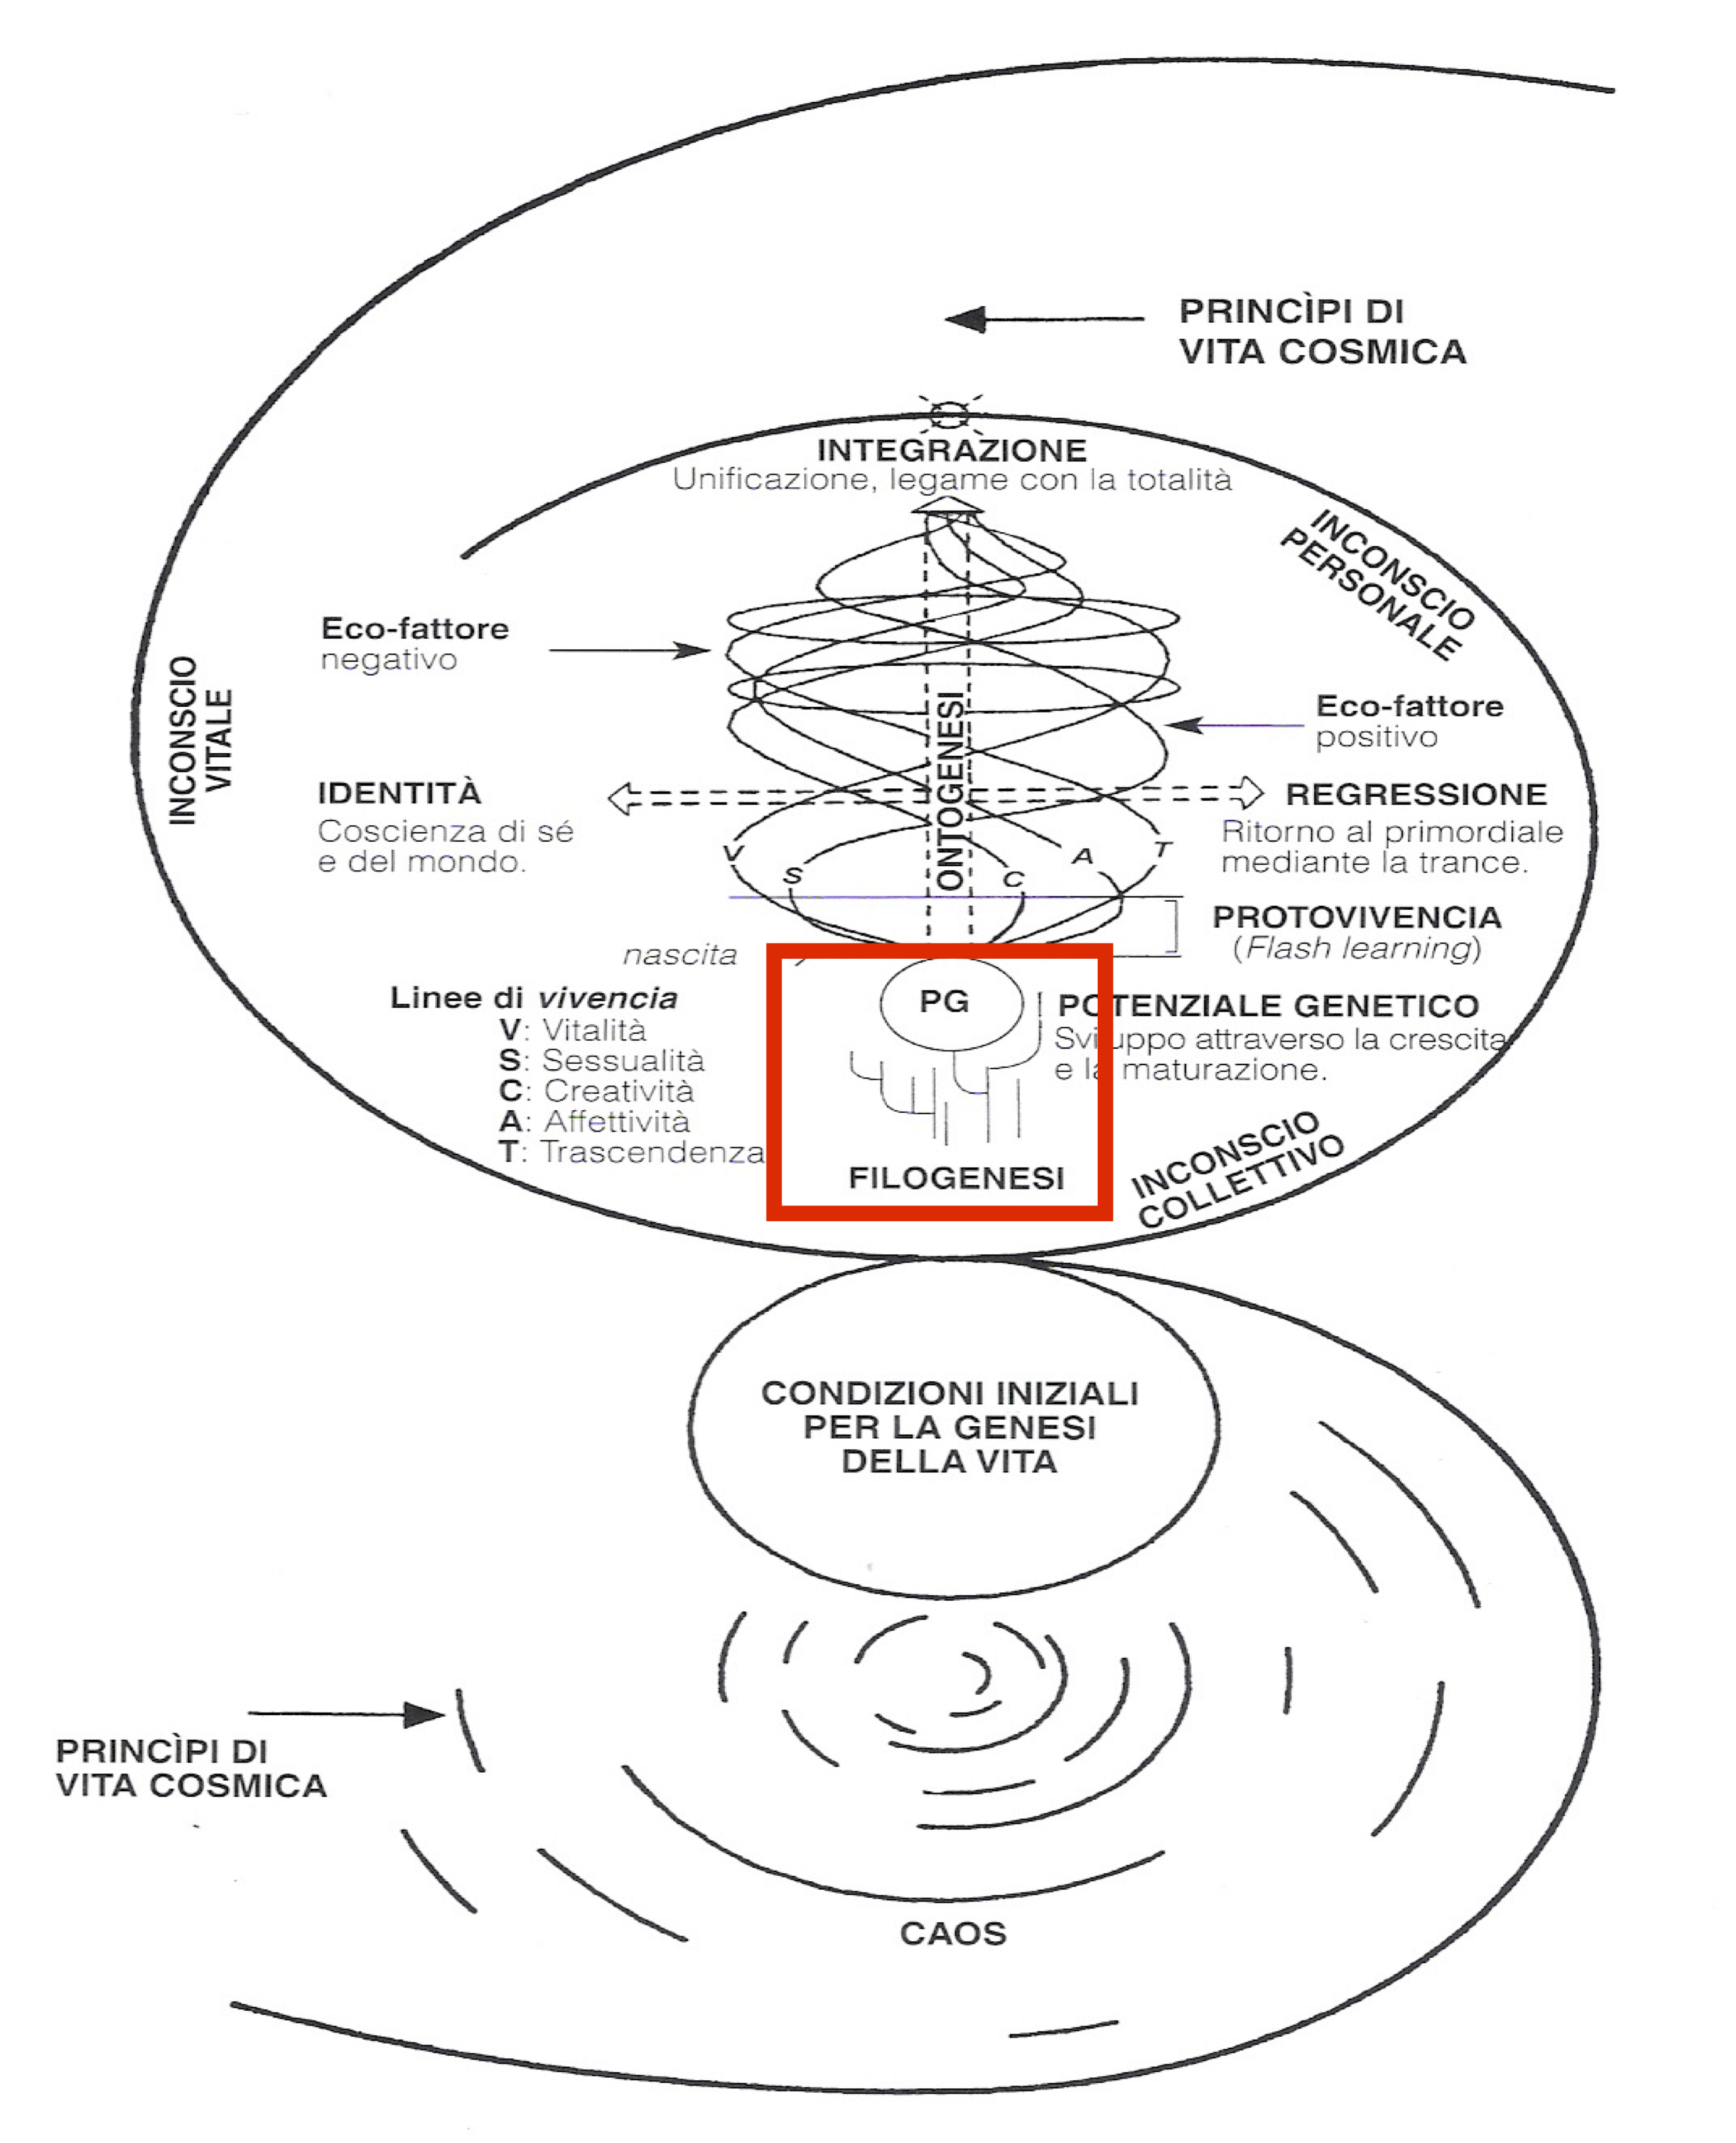
\includegraphics[width=0.5\linewidth]{./figs/biologischeAspectenBiodanzaDeelII} 

}

\caption{Model of Biodanza and Phylogenesis}\label{fig:modelPhylo}
\end{figure}

We start this chapter with two sections that are more technical and focus on the concepts related to Phylogenesis and Evolution introduced in the reader of the Biodanza teacher training ``Module IV: Biological aspects of Biodanza''. We conclude this chapter with a more philosophical section on evolution, humanity and Biodanza.

\hypertarget{phylogenesis}{%
\section{Phylogenesis}\label{phylogenesis}}

All species evolved from the same ancestral population of cells.
This is also referred to as the same Last Universal Common Ancestor (LUCA).
In the tree of life the evolutionary relations are summarized between different organisms (and groups of organisms). All living beings eventually can be traced back to the last universal common ancestor who is located at the root of the tree, see Figure \ref{fig:treeOfLifeBis}.

\begin{figure}

{\centering 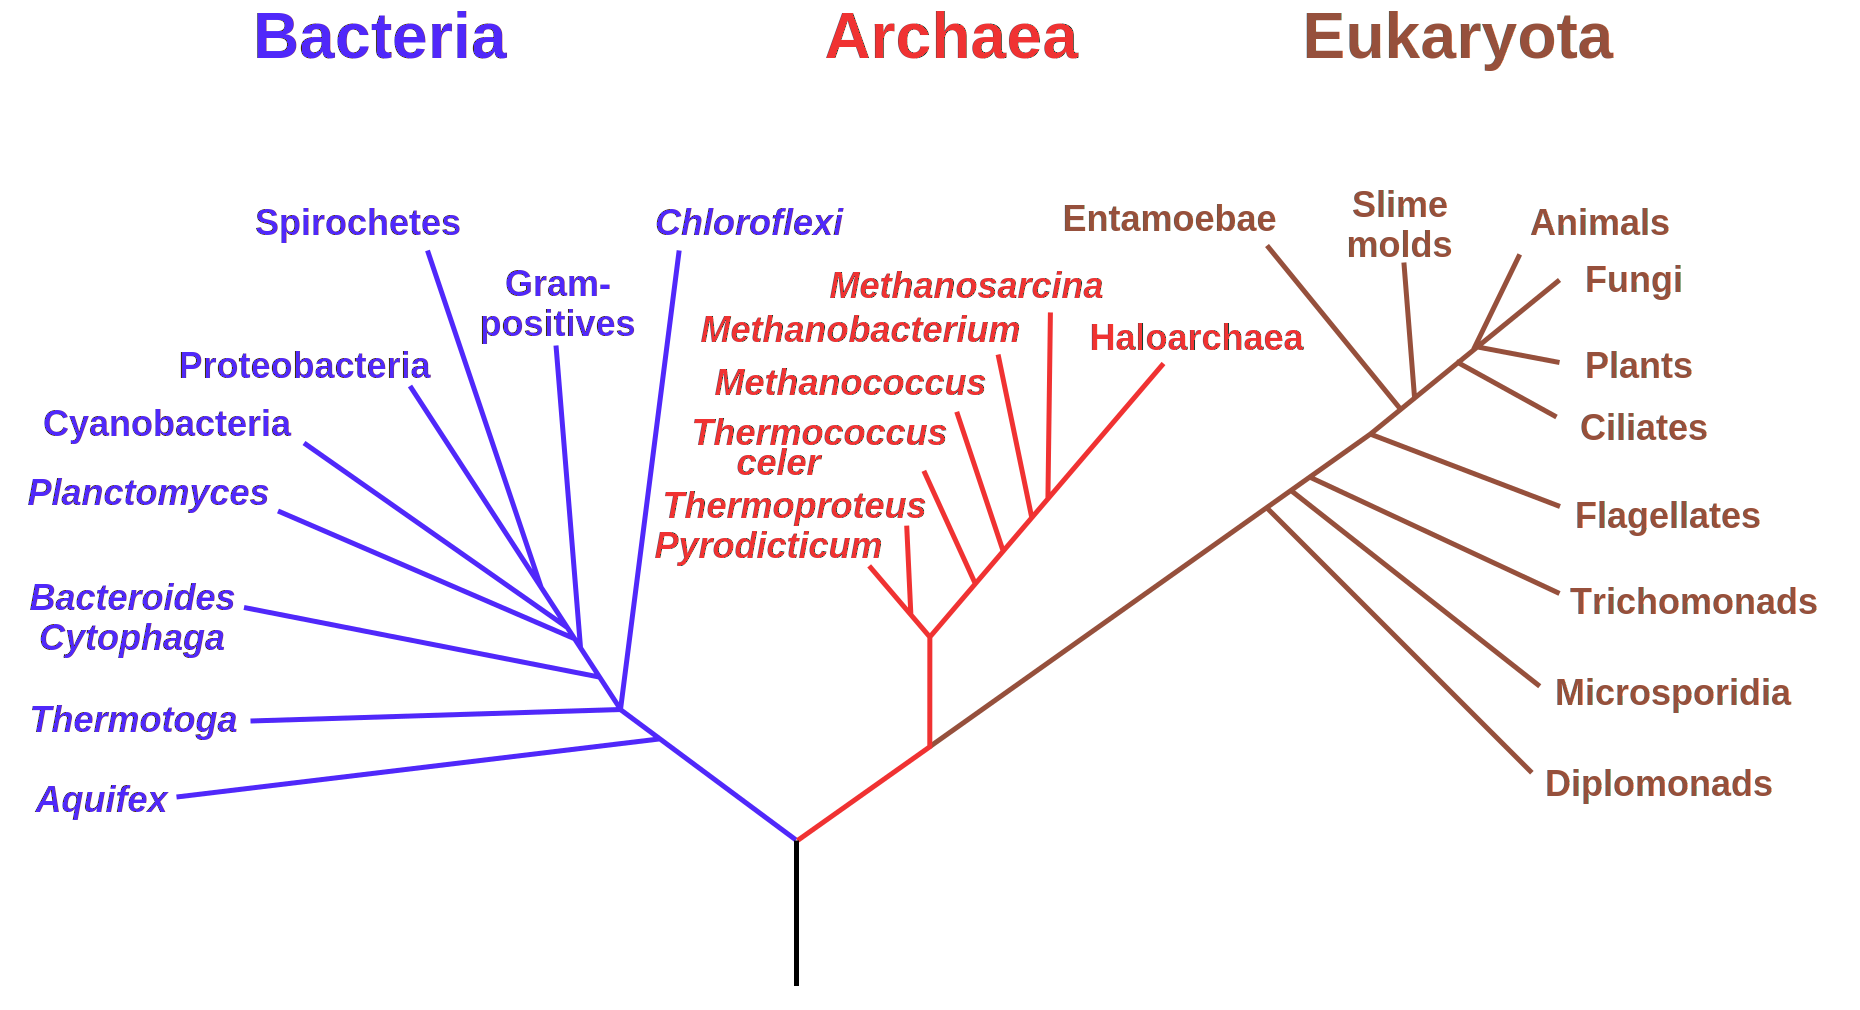
\includegraphics[width=1\linewidth]{./figs/Phylogenetic_tree} 

}

\caption{The tree of life is one of the most important organizing principles in biology. It shows the evolutionary relationships among different organisms and that all living beings eventually can be traced back to the last universal common ancestor who is located at the root of the tree (Source: wikipedia)}\label{fig:treeOfLifeBis}
\end{figure}

Phylogenesis is the process of the origin of all species from the tree of life from LUCA.

Rolando Toro refers to the origin of species and adaptation to the environment as evolutionary differentiation.

\hypertarget{timescale}{%
\subsection{Timescale}\label{timescale}}

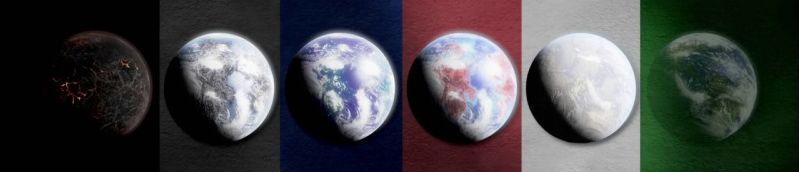
\includegraphics{./figs/liferockystartstrip.jpeg}

\begin{longtable}[]{@{}llllll@{}}
\toprule()
4.5 BYA & 4.3 BYA & 3.8 BYA & 3.5 BYA & 540 MYA & 520 MYA \\
\midrule()
\endhead
& & & & & \\
\bottomrule()
\end{longtable}

(Source: naturedocumetaries.org)

At its origin about 4.5 Billion Years Ago (BYA) the Earth was black, a hot basalt rock and dust in a cold vacuum.
As the Earth cooled down she became Grey Earth (4.3 BYA) as she was mainly covered by granite and rocks. Another 500 million years later she was covered with liquid water: Blue Earth (3.8 BYA).

In only 300 million years she radically changed into Red Earth (3.5 BYA) due to life. Indeed, cyanobacteria emerged that can do photosynthesis and produce oxygen, a very reactive molecule. This led all free iron in the ocean to precipitate as iron oxide or rust (red). There was an explosion of the number of minerals, they went from approximately 250 to more than 5000 mineral species. Oxygen also caused a mass extinction because only few organisms could cope with its highly reactive nature. The coming 3 billion years life on Earth stayed relatively similar.

Around 540 MYA Earth was struck by a large ice age, White Earth.
Again leading to a mass extinction due to the cold. However, volcanic activity came to the rescue by producing greenhouse gasses and an atmosphere that could retain more heat.

In less than 20 million years (MY) Earth radically changed again and turned into Green Earth (520 MYA). There was an explosion of life, and life suddenly evolved from being mainly unicellular to complex multicellular forms.

\hypertarget{endosymbiosis}{%
\subsection{Change Point: Eukaryotic Cells and Increase of Oxygen}\label{endosymbiosis}}

There are two archetypes of cells:

\begin{itemize}
\tightlist
\item
  Prokaryota, simple cells of a size of 0.1 to 5.0 \(\mu m\) with DNA that is lying freely in the cell cytosol (the fluid in the cell), see Figure \ref{fig:prokaryotaCell} and
\end{itemize}

\begin{figure}

{\centering 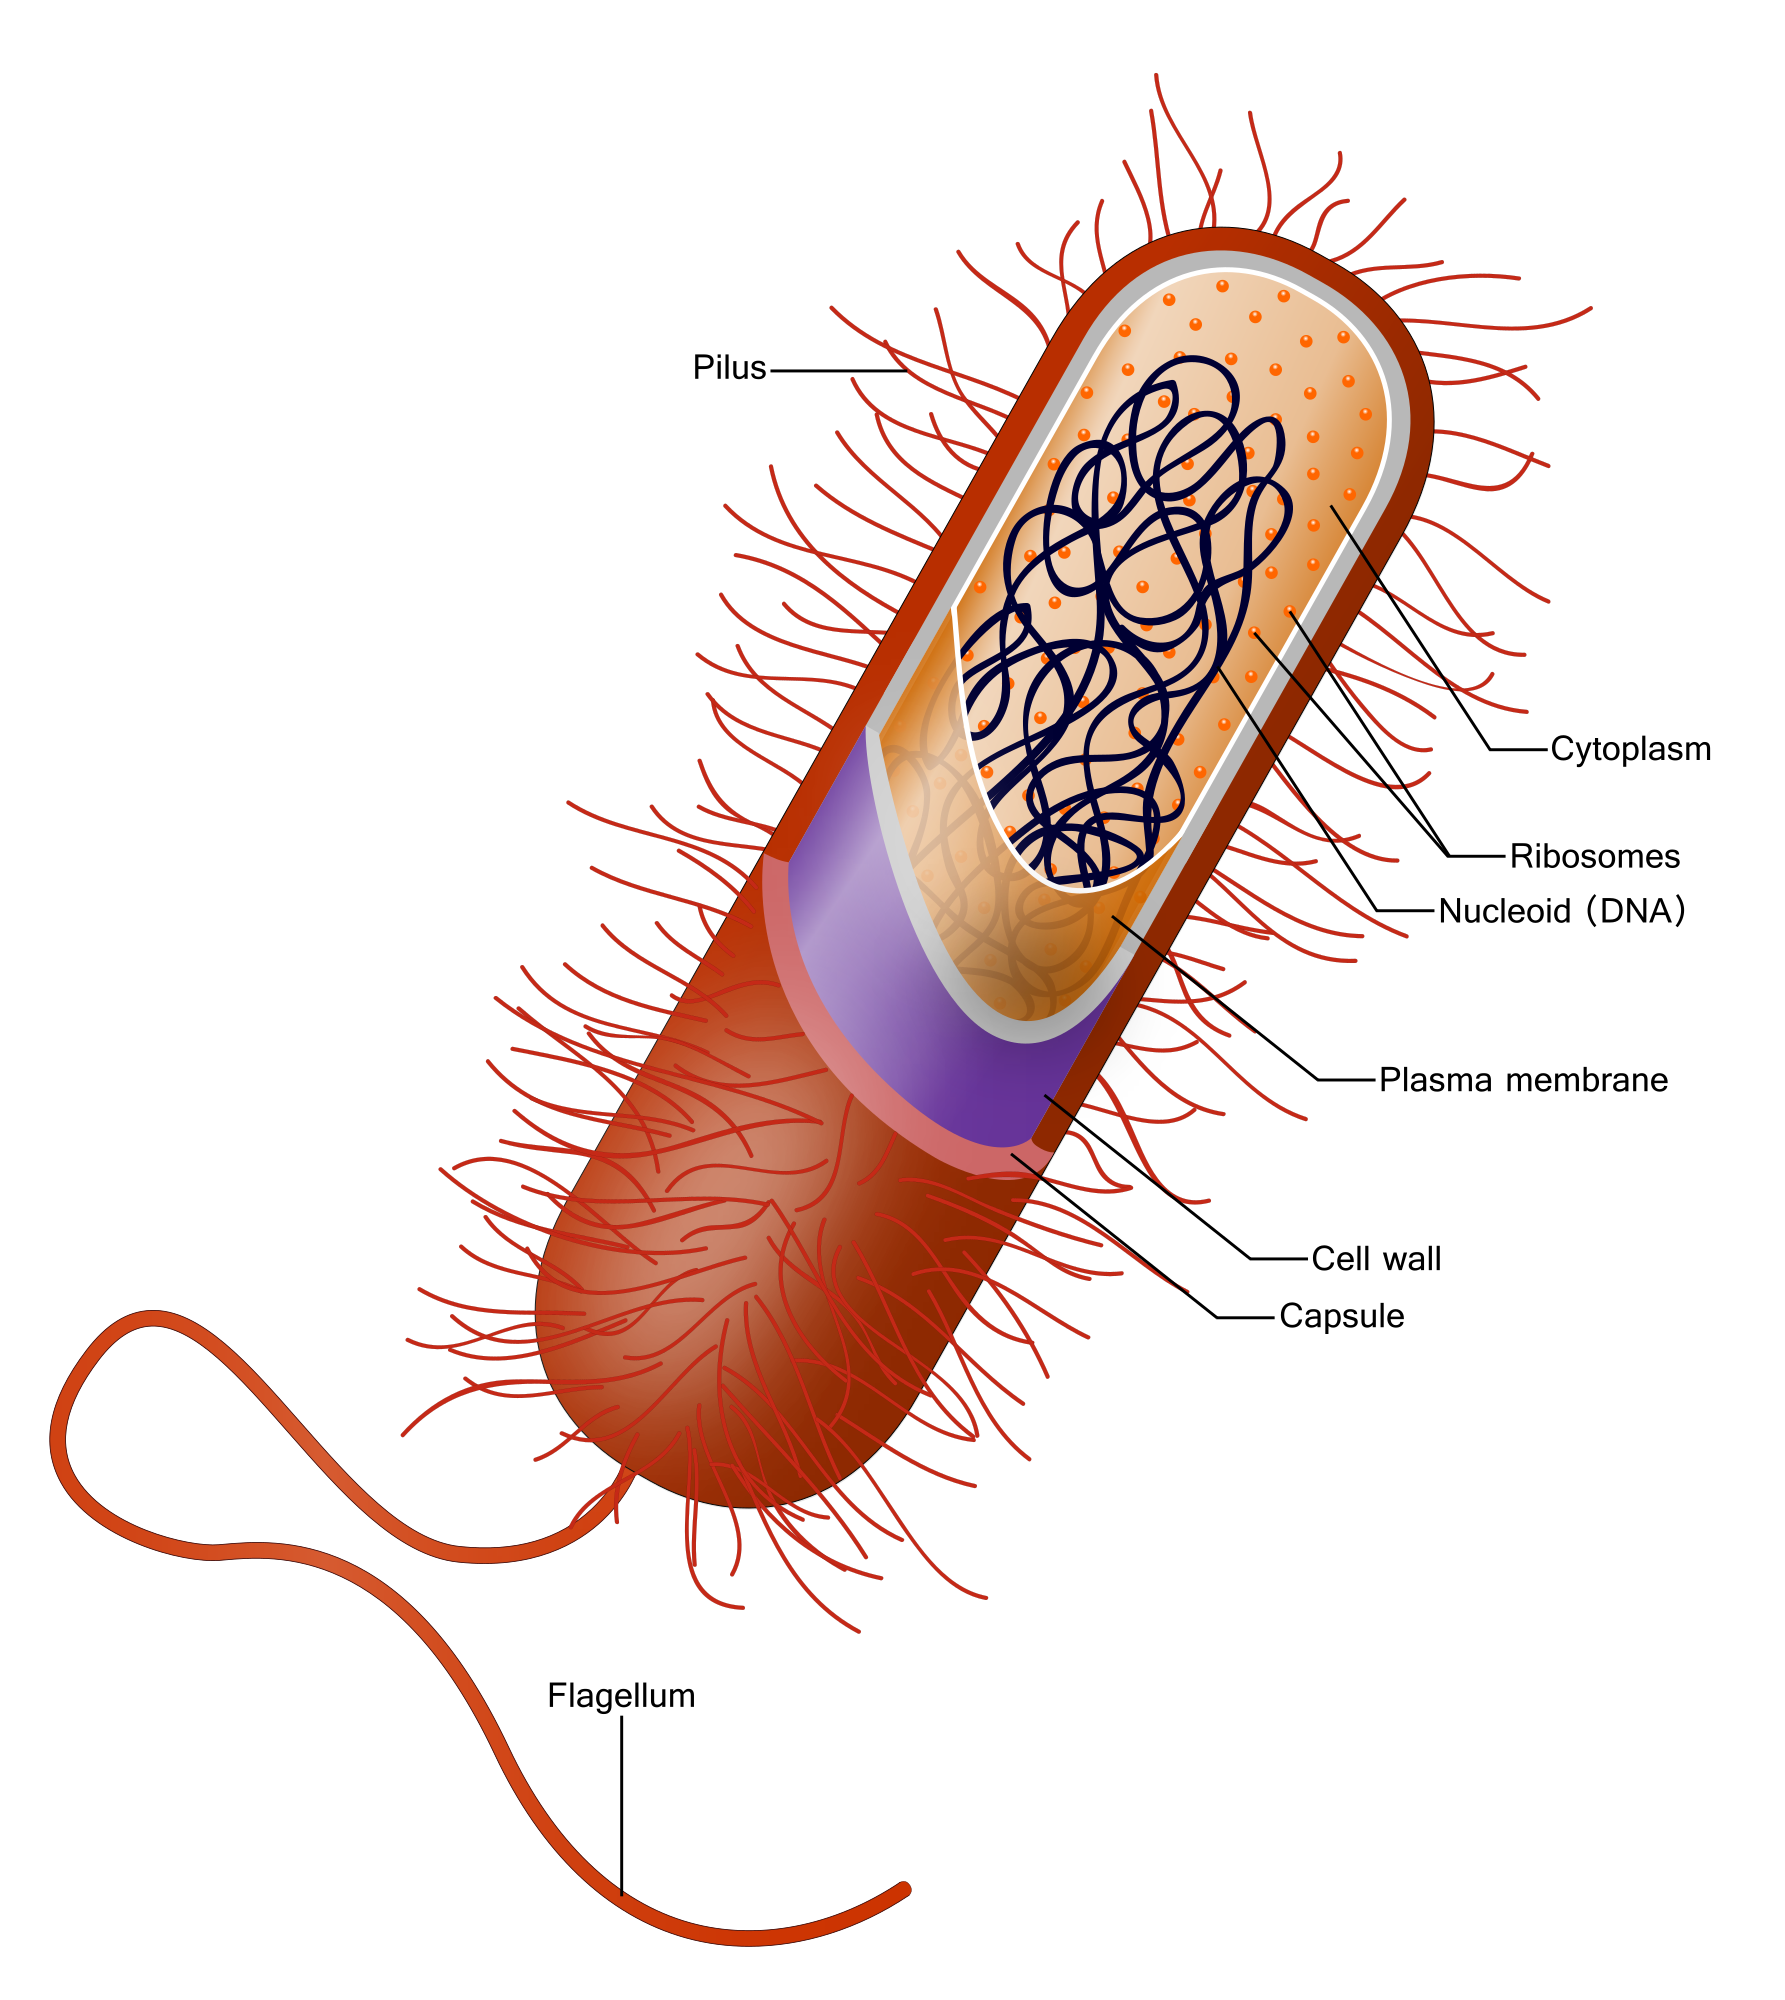
\includegraphics[width=0.5\linewidth]{./figs/prokaryoteCell} 

}

\caption{Diagram of a typical prokaryotic cell. The cell is simple, the DNA is lying free in the cell (Source: Ali Zifan, Wikipedia)}\label{fig:prokaryotaCell}
\end{figure}

\begin{itemize}
\tightlist
\item
  Eukaryota are larger and more complex cells, 10-100 \(\mu m\) in size. They have a variety of internal membrane-bound structures, called organelles, and a cytoskeleton, which play an important role in defining the cell's organization and shape. Eukaryotic DNA is stored in chromosomes. A chromosome is a long DNA molecule that is stored in a compact form. A chromosome contains a part or all of the genetic material of an organism. Human cells have 46 chromosomes, i.e.~23 chromosome pairs. Each pair consists of one copy from our biological mother and one from our biological father. The chromosomes are located in the cell nucleus, which is the organelle maintaining the integrity of chromosomes and thus of our genes, and plays an important role in the regulation of gene expression and of the activities of the cell. See Figures \ref{fig:animalCell} and \ref{fig:plantCell}.
\end{itemize}

\begin{figure}

{\centering 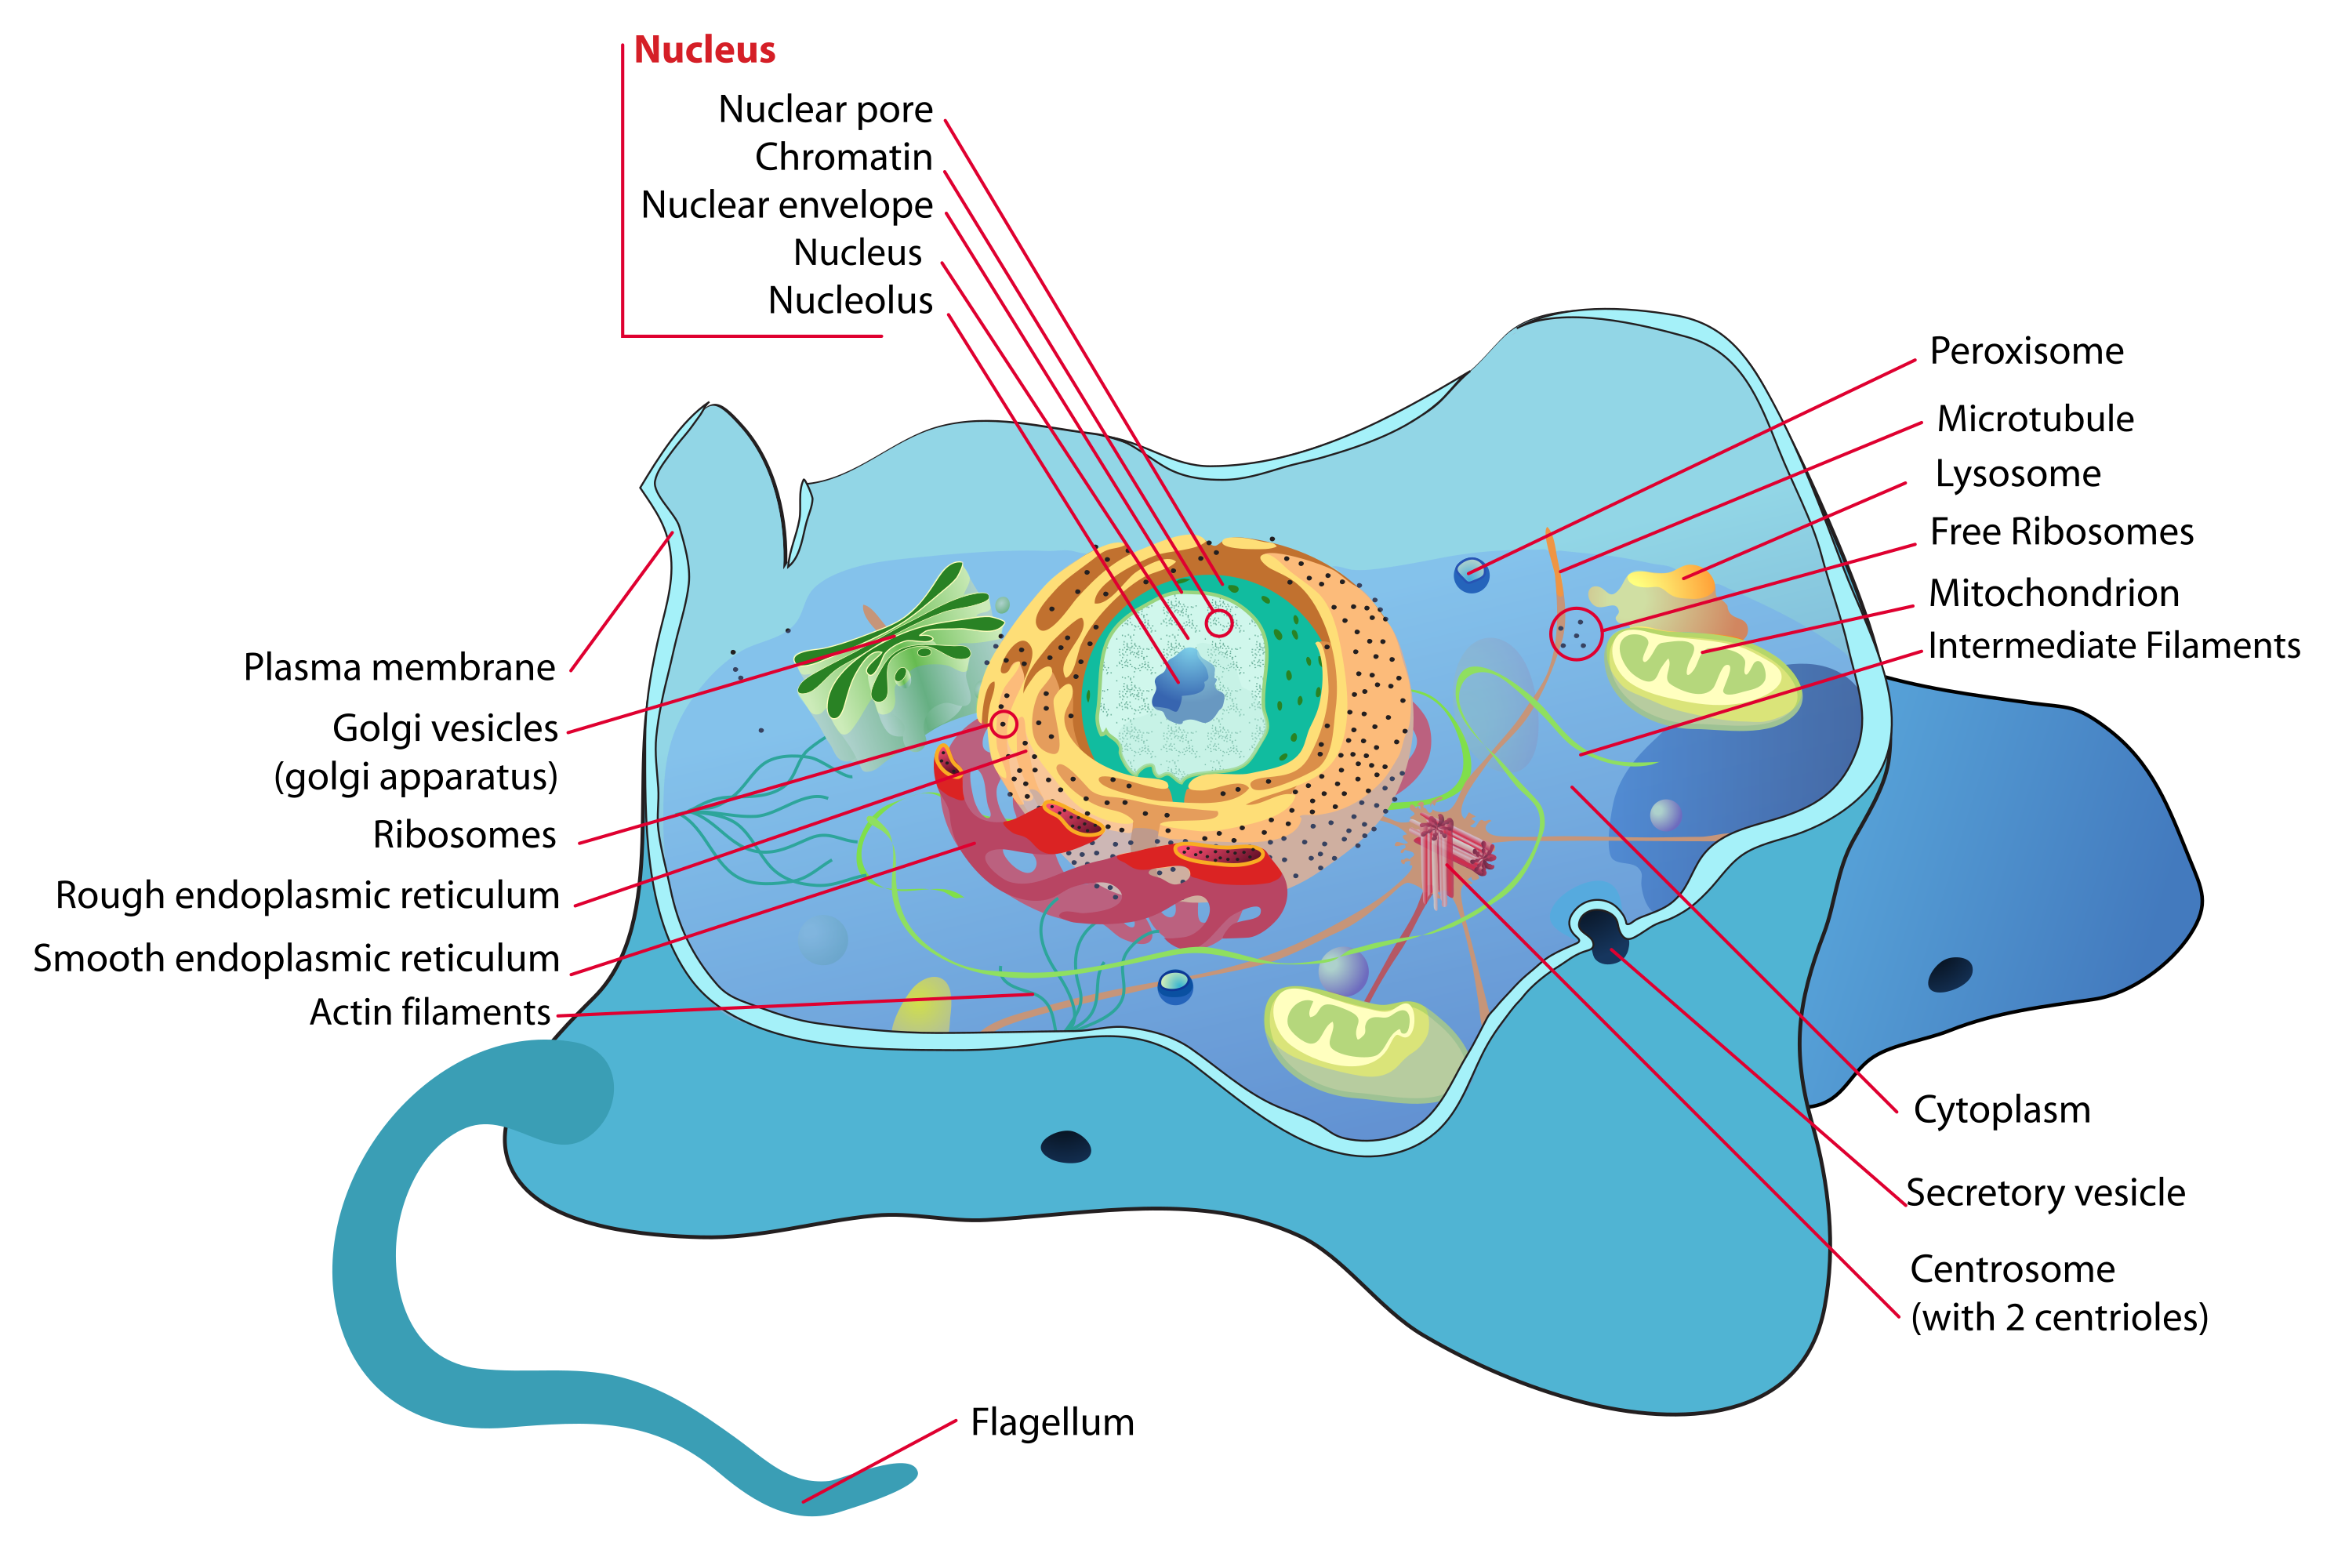
\includegraphics[width=0.5\linewidth]{./figs/animalCell} 

}

\caption{Diagram of a typical animal cell. Animal cells are eukaryotic cells. They are typically much larger than those of prokaryotas. They have a variety of internal membrane-bound structures, called organelles, and a cytoskeleton, which play an important role in defining the cell's organization and shape. Eukaryotic DNA is divided into chromosomes, that are located in the cell nucleus, which is the organelle maintaining the integrity of genes, and plays an important role in the regulation of gene expression and of the activities of the cell. (Source: Mariana Ruiz Villarreal, Wikipedia)}\label{fig:animalCell}
\end{figure}

\begin{figure}

{\centering 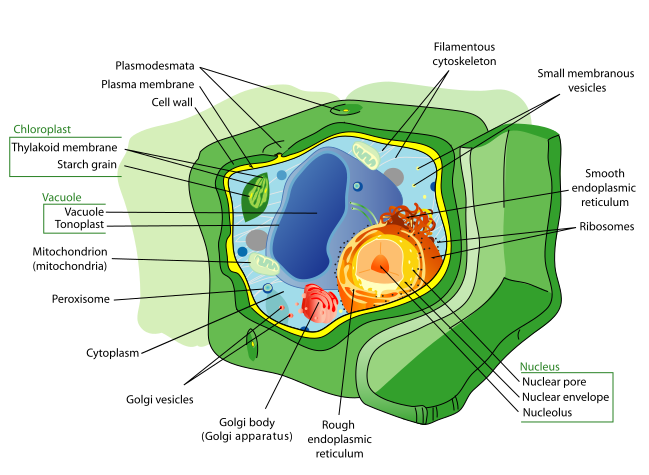
\includegraphics[width=0.5\linewidth]{./figs/plantCell} 

}

\caption{Diagram of a typical plant cell. Animal cells are eukaryotic cells. They are typically much larger than those of prokaryotas. They have a variety of internal membrane-bound structures, called organelles, and a cytoskeleton, which play an important role in defining the cell's organization and shape. Eukaryotic DNA is divided into chromosomes, that are located in the cell nucleus, which is the organelle maintaining the integrity of genes, and plays an important role in the regulation of gene expression and of the activities of the cell. Plant cells also have a cell wall and chloroplasts that can perform photosynthesis. (Source: Mariana Ruiz Villarreal, Wikipedia)}\label{fig:plantCell}
\end{figure}

From 3.5 BYA - 540 MYA we find mainly prokaryotic and some simple eukaryotic organisms in fossils and life was mainly unicellular.

Eukaryotic cells are believed to be generated by endosymbiosis, i.e.~a symbiotic relationship where one organism lives inside the other, which is beneficial for both organisms.

The process of endosymbiosis that led to eukaryotic cells is displayed in Figure \ref{fig:endosymbiosis}.

\begin{figure}

{\centering 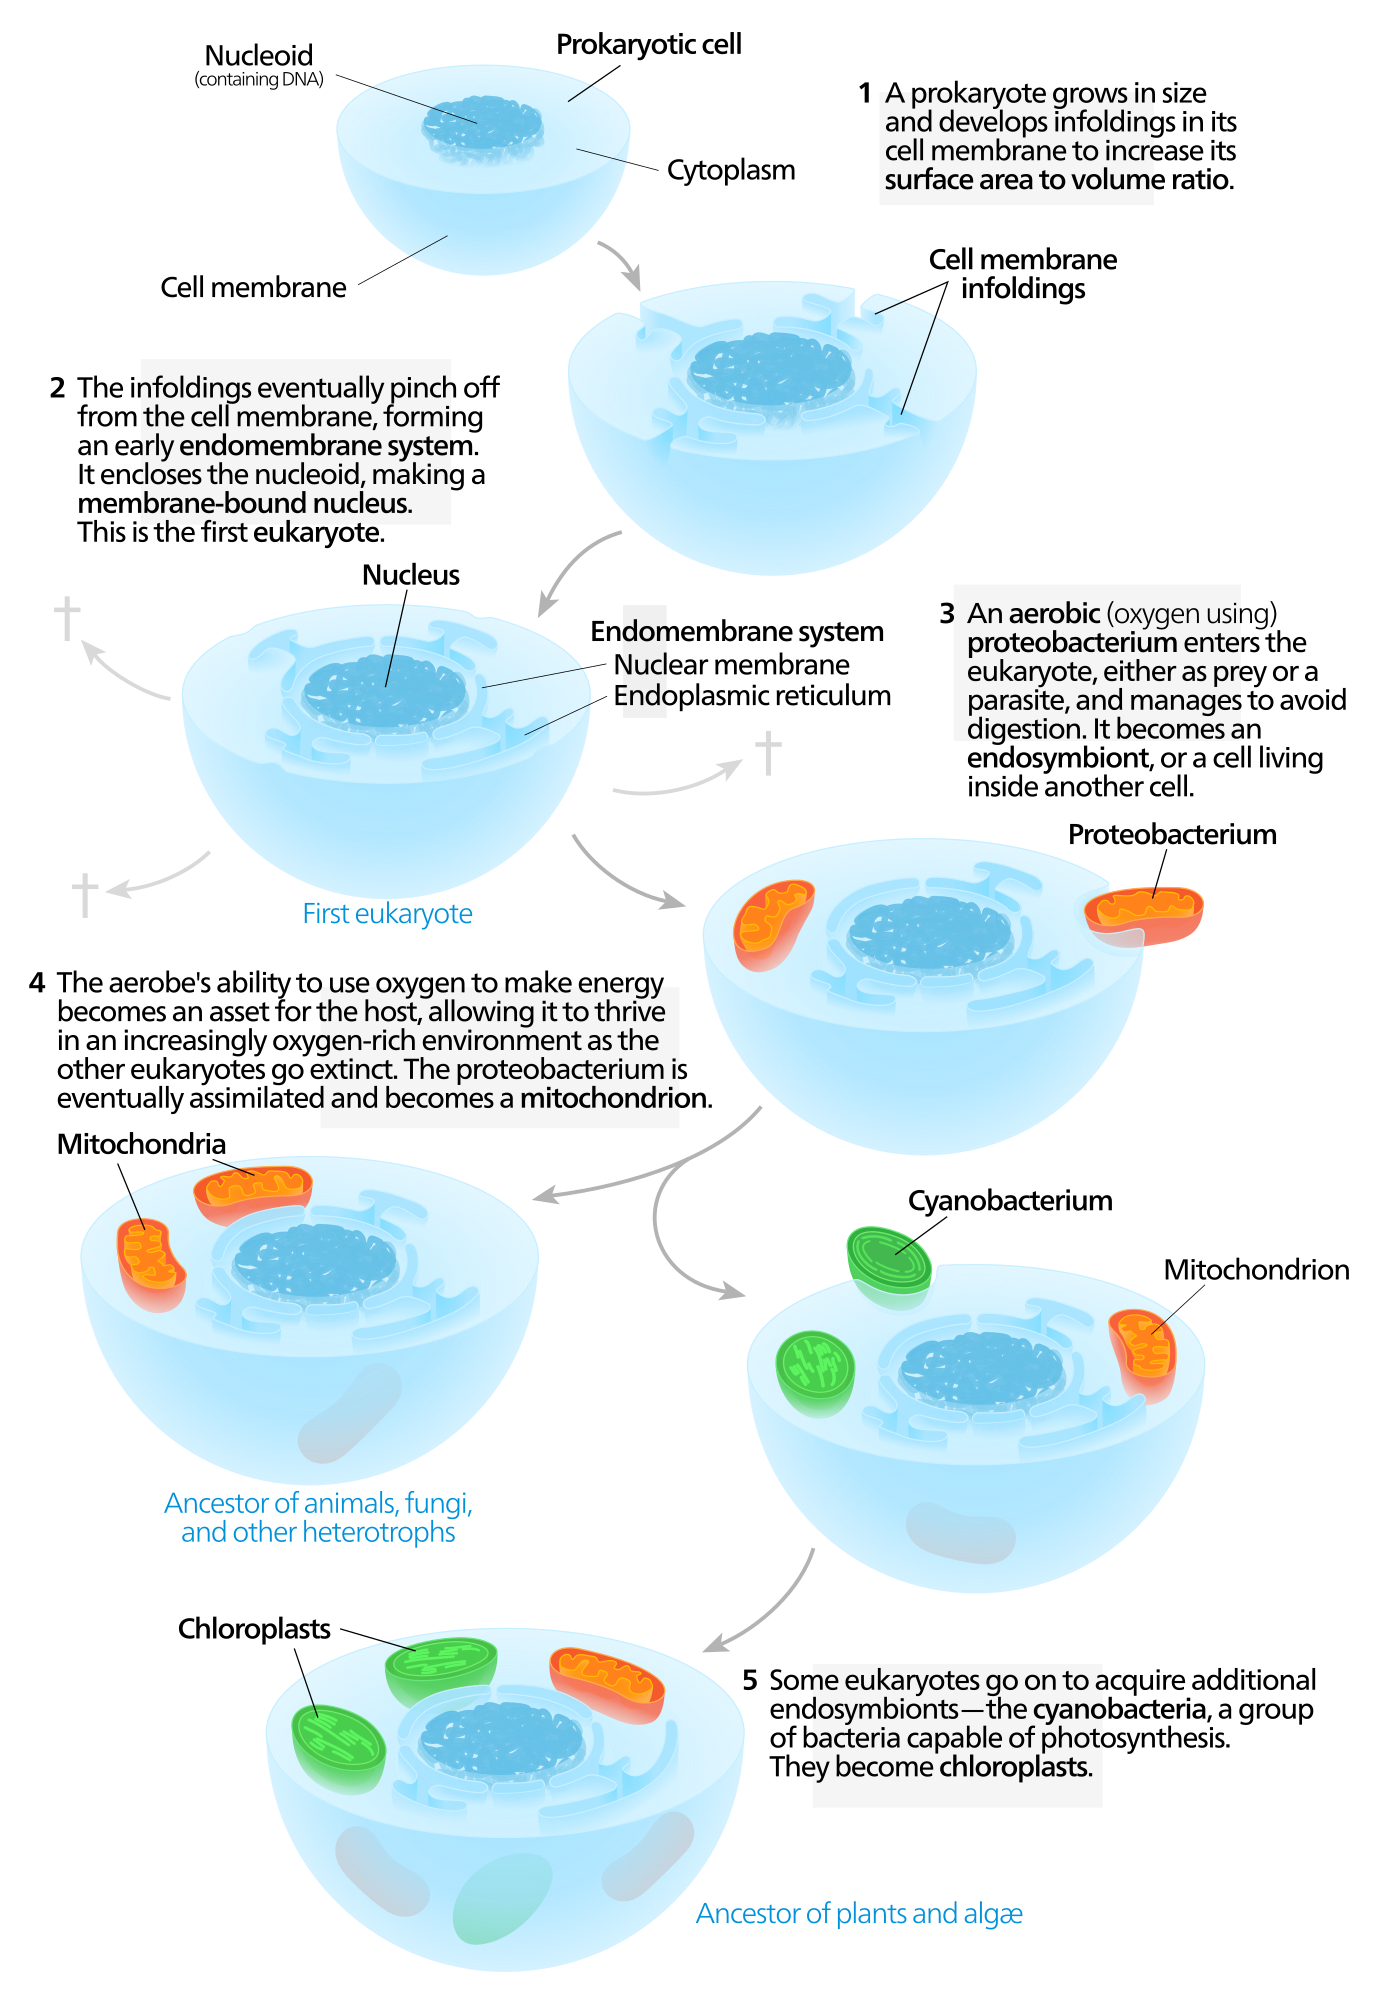
\includegraphics[width=0.8\linewidth]{./figs/endosymbiosis} 

}

\caption{Genesis of eukaryotic cells (Source: wikipedia)}\label{fig:endosymbiosis}
\end{figure}

First an anaerobic\footnote{Anaerobic: living in the absence of oxygen} prokaryotic cell was assumed to have grown and to have developed membrane systems inside the cell, which gave rise to the formation of the nucleus. At a certain point of time this large prokaryotic cell with internal membrane systems must have ingested an aerobic\footnote{Aerobic: oxygen using and respiration with oxygen provides more energy} proteobacterium, which managed to avoid digestion. The two cells started with an endosymbiotic relation.

The proteobacterium provided the host cell with additional energy through the synthesis of ATP by metabolizing carbohydrates and lipids using oxygen and the host cell fed the proteobacterium with these bio-molecules. This gave the endosymbiotic pair the ability to grow further in size and to thrive in the oxygen rich environment of planet Earth that was established during the Cambrian era that started 540 million years ago. The increase of oxygen is believed to be one of the major triggers that gave rise to the ``biological big bang'' that led to an explosion of novel species and the emergence of all large groups\footnote{Large groups of a kingdom are more formally referred to as \emph{phyla}} in the animal kingdom \citep{he2019}.

During their endosymbiotic evolution the proteobacterium gradually handed over many genes to the cell nucleus, and became under regulation of the nucleus. It eventually evolved to mitochondria, the organelles that are the energy plants of a cell. So, we inherit more from mother than father: we inherit our cell structure as well as our energy system, i.e.~our mitochondria and their remaining DNA, from mother side through her egg cell.

For plant cells, a second endosymbiotic event must have occurred with eukaryotic cells and cyanobacteria. The ingested cyanobacteria has evolved in a similar way into chloroplasts, which give plants the ability for photosynthesis and led them become the most successful life form of the globe. Fossil evidence of land plants dates back to 485 MYA - 420 MYA, however, phylogenetic analysis also suggests an earlier origin in the Cambrian \citep{StrotherFoster2021}.

Other key differences between Prokaryota and Eukaryota are in terms of their reproduction.
For Prokaryota that only takes place by cell division. A mutation in the DNA is thus fixed in all daughter cells. While nearly all Eukaryota have a phase of sexual reproduction. They are diploid organisms, i.e.~they have two copies of each gene, one from fathers' and mothers' side. This enables successive mutations to be made in one copy because another functional copy of the gene is available. Moreover during sexual reproduction recombination of chromosomes occurs, i.e.~reshuffling of paternal and maternal genes, which leads to much more variation.

The Eukaryota further evolved in protists, which are unicellular organisms, fungae, plants and animals.

\hypertarget{evolution}{%
\section{Evolution}\label{evolution}}

How does the evolution of LUCA to all species of the tree of life occurred?
Evolution is largely driven by variability and selection.

\hypertarget{variability-and-selection}{%
\subsection{Variability and Selection}\label{variability-and-selection}}

Variation occurs, among others, through errors in the copying of DNA for cell division of prokaryotic cells and gamete\footnote{Gamete: sperm or egg cell} production for eukaryotic cells (see Figure \ref{fig:dnaPolymerase}).

\begin{figure}

{\centering 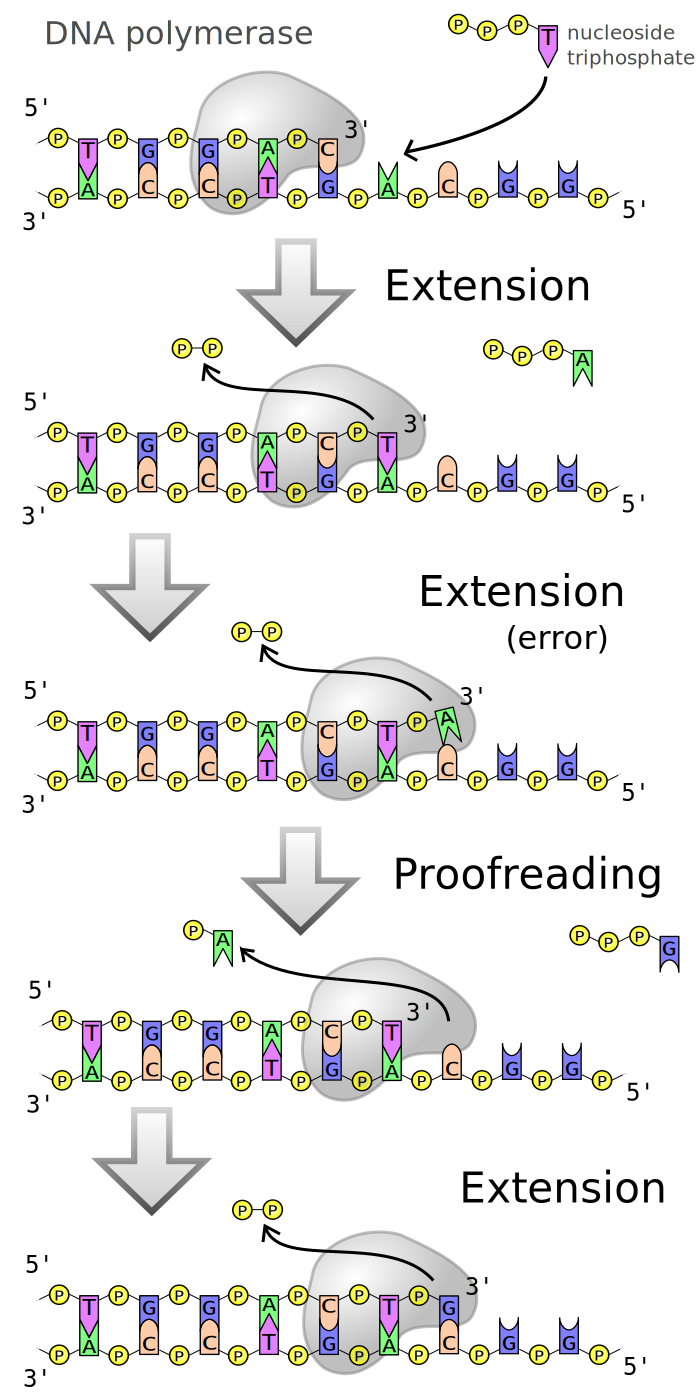
\includegraphics[width=0.45\linewidth]{./figs/DNA_polymerase} 

}

\caption{Copying of DNA by DNA-polymerase. DNA polymerase extends a DNA strand by incorporating a complementary nucleoside-tri-phosphate and splitting two of the three phosphate groups. Note, again the link between energy and information. Errors are often corrected by proofreading. However, some of the errors remain.}\label{fig:dnaPolymerase}
\end{figure}

The error margin of DNA replication is 1 error per billion base pairs that are copied, which can lead to point mutations. Note, that we humans have a genome size of about 6.4 billion base pairs.

Other sources of variability are

\begin{itemize}
\tightlist
\item
  Insertions or deletions, i.e.~base pairs that are added or removed, respectively.
\item
  Recombination, reshuffling of genetic traits, e.g.~during sexual reproduction
\end{itemize}

Most mutations are neutral, i.e.~the mutated codon encodes for the same amino acid. Neutral mutations can be used as a molecular/genetic clock to tell how far apart two species are in an evolutionary sense.

But, mutations are not always neutral! For instance, sickle cell anemia is caused by one point mutation in hemoglobin (see Figure \ref{fig:sickleCell1} and \ref{fig:sickleCell2}). A thymine is mutated to an adenine, which results in a codon that encodes for the amino acid valine instead of glutamic acid. This causes dramatic changes to the 3D structure of the hemoglobin protein and causes a deformation of the red blood cells from a round to sickle shape, which leads to anemia.

Why does this mutation remain? It mainly occurs in Africa, where the mutation for sickle cell anemia is selected because it makes affected individuals resistant against malaria, which gives them a evolutionary competitive advantage despite their anemia. However, offspring who inherit the mutation of both parents are not viable. Therefore, the regular variant of hemoglobin also remains.

\begin{figure}

{\centering 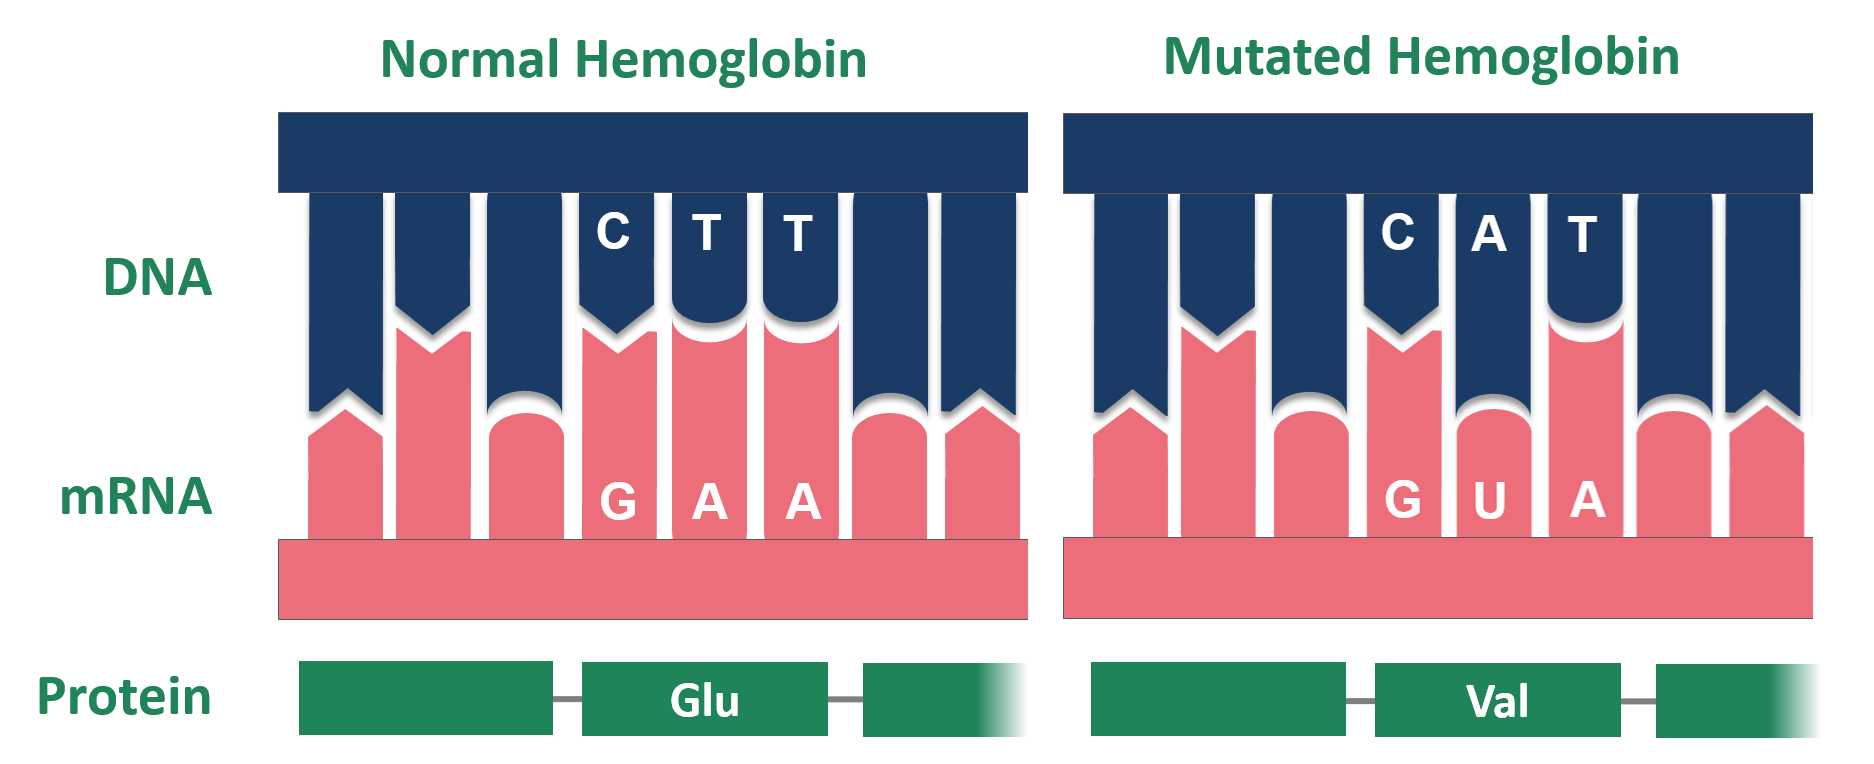
\includegraphics[width=0.45\linewidth]{./figs/sickleCellWikipedia2} 

}

\caption{Mutation of Hemoglobin in patients with sickle cell anemia (Source: Wikipedia)}\label{fig:sickleCell1}
\end{figure}

\begin{figure}

{\centering 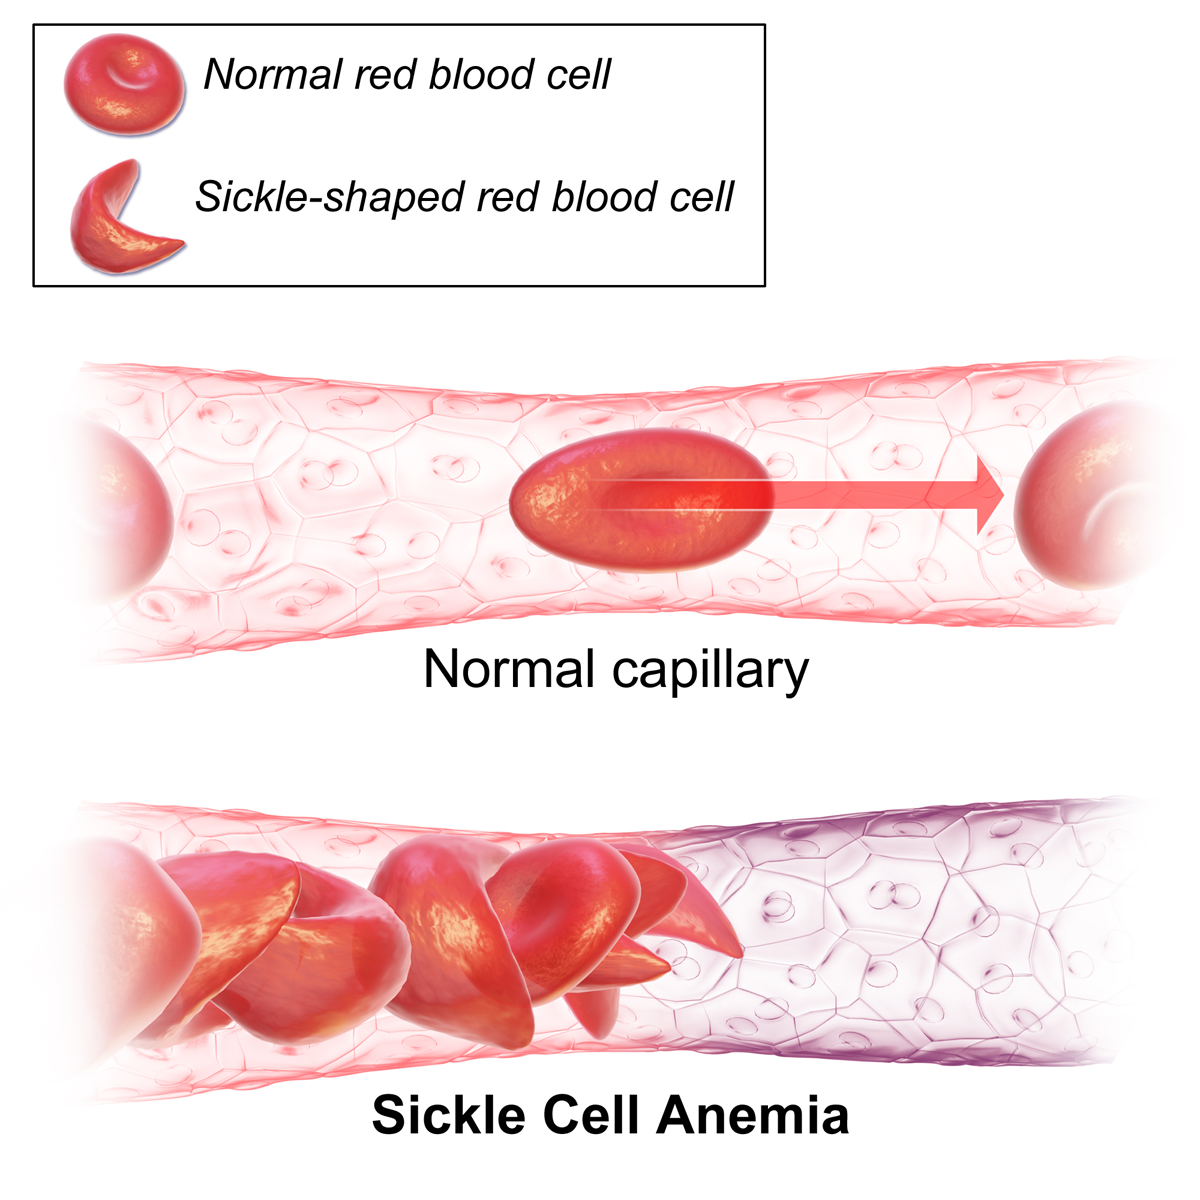
\includegraphics[width=0.45\linewidth]{./figs/Sickle_Cell_Anemia_wiki3} 

}

\caption{Deformed red blood cells in patients with sickle cell anemia (Source: Wikipedia)}\label{fig:sickleCell2}
\end{figure}

Hence, evolution is a natural process that is driven by two opposing forces: variation and selection.

Variation occurs by spontaneous copy errors in genetic code or mutations, among others.

Selection occurs upon ecofactors: Is a mutation beneficial or harmful for a particular organism in its specific environment?
The odds on fixation of the mutation thus depends on the reproductive success.

The process of genetic variation and selection can eventually lead to evolution of new species upon many generations.

\hypertarget{genetic-drift}{%
\subsection{Genetic Drift}\label{genetic-drift}}

Another important process for the origin of species is genetic drift. This are random fluctuations of alleles, which are particular sequence variants of a gene. Genetic drift is particularly strong in small populations. As opposed to selection it is not adaptive.

New species will thus originate more quickly when a small fraction of the population gets isolated in a new environment.

\hypertarget{horizontal-gene-transfer}{%
\subsection{Horizontal Gene Transfer}\label{horizontal-gene-transfer}}

Horizontal gene transfer, which is non-sexual transfer of genetic information between two distinct organisms, is also important for the evolutionary process.

This is very common between Prokaryota, i.e.~eubacteria and archaea bacteria, think on the super bugs in hospitals that acquired resistance to multiple antibiotics. It also occurs between Eukaryota. Mainly in protists, which are unicellular organisms with a nucleus. As well as between Prokaryota on the one hand and Eukaryota on the other hand.

\hypertarget{endosymbiosis-1}{%
\subsection{Endosymbiosis}\label{endosymbiosis-1}}

Endosymbiosis is also a very important driver of evolution. Niles Eldredge and Stephen Jay Gould have shown that the fossil record indicates that evolution happens in bursts: it is slow most of the time until suddenly rapid changes occur over a brief time \citep{margulis1999}. According to Lynn Margulis this can be explained due to endosymbiosis, where one species starts to live within another species, which is a source of evolutionary novelty that can give rise to an explosion of novel life forms. We already touched in more detail upon an important endosymbiosis event in section \ref{endosymbiosis}.

\hypertarget{teleonomy}{%
\subsection{Teleonomy}\label{teleonomy}}

The term teleonomy means that evolution only has the primitive goal to maintain and reproduce the species, and, that it thus has no other purpose and thus also no direction.

When complex organs and organisms originate it might seem as if there is a direction or purpose, but, that is not the case! A good example is the development of an eye, see Figure \ref{fig:evolutionEye}.

\begin{figure}

{\centering 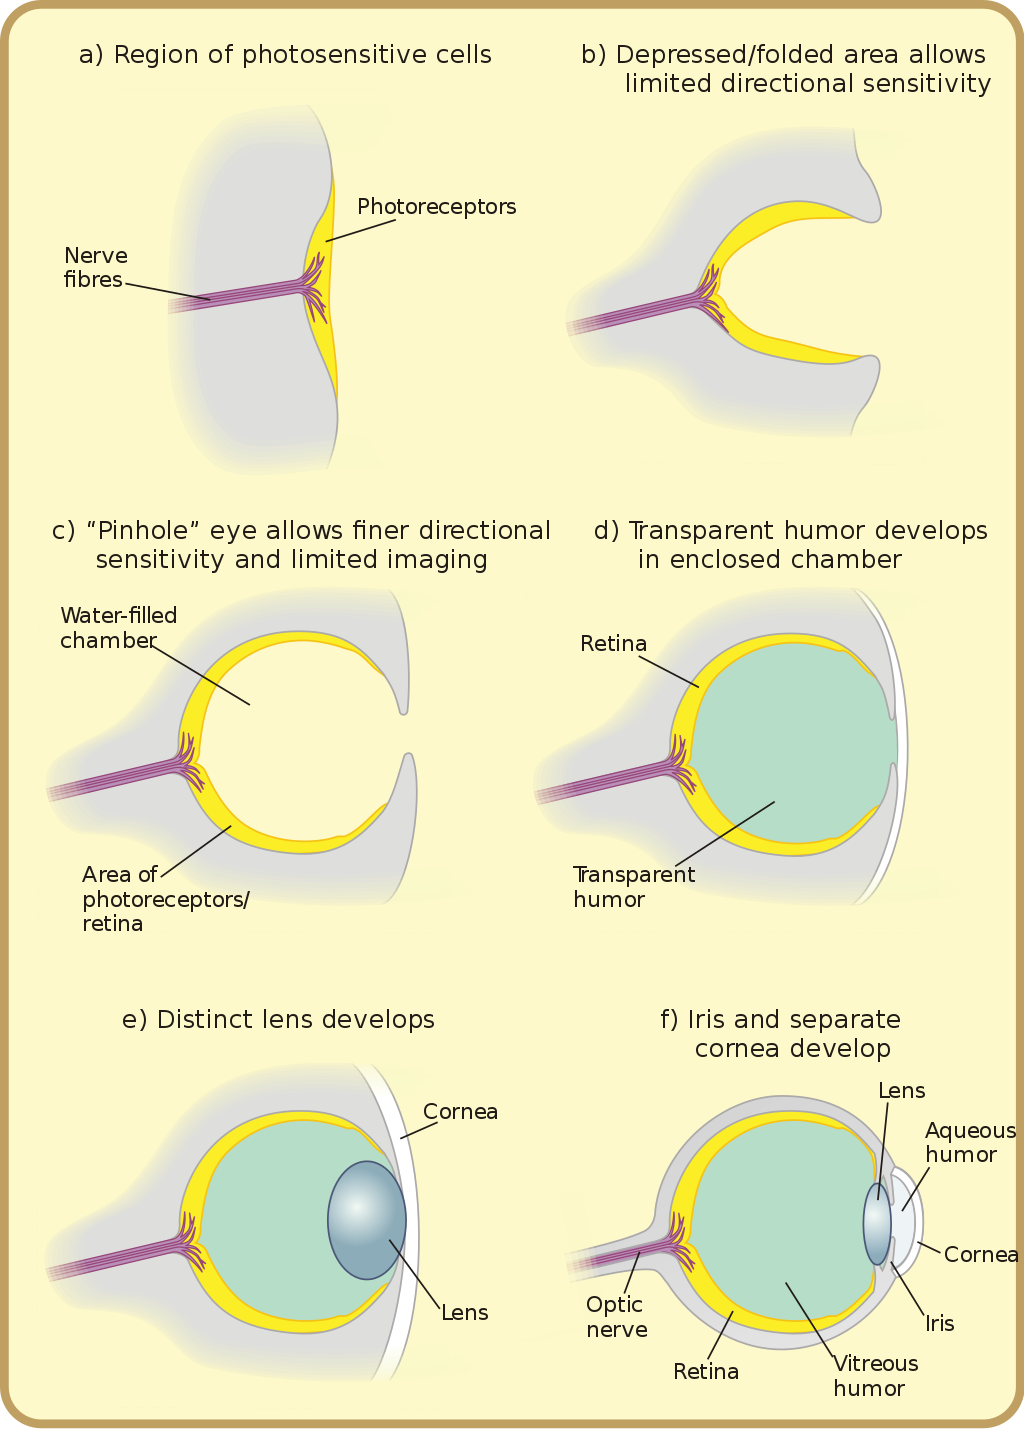
\includegraphics[width=0.45\linewidth]{./figs/evolutionEye} 

}

\caption{The evolution of an eye (Source: Wikipedia)}\label{fig:evolutionEye}
\end{figure}

Indeed,

\begin{itemize}
\item
  The eye is not developed by evolution with the purpose to see.
\item
  The eye only has the function to see.
\item
  It is the result of a gradual process where each adaptation gave a reproductive advantage in a particular environment.
\item
  In another environment it can be no longer functional and than it might disappear or might become dysfunctional, e.g.~moles eyes.
\end{itemize}

Hence, the origin of a species is the result of evolution, but, not the purpose of evolution. Evolution is thus adaptation with as sole goal maintenance and reproduction.

From the distribution of the complexity of species in Figure \ref{fig:distributionComplexity}, it is clear that the most abundant species in number always has been bacteria.
Indeed, evolution has no direction.
The distribution of complexity at present, however, has a tail to the right.
This mainly stems from the fact that there is lower bound of complexity of living organisms. Hence, evolution could not generate organisms with a complexity below this lower bound and it therefore only seems as if it slightly favors increasing complexity.



\begin{figure}

{\centering 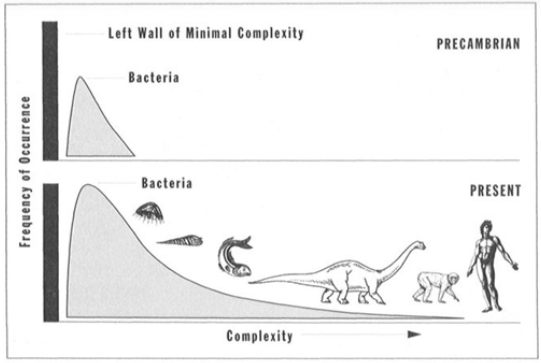
\includegraphics[width=0.45\linewidth]{./figs/selectionNoDirectionDef} 

}

\caption{Distribution of complexity of species \citep{gould1997}}\label{fig:distributionComplexity}
\end{figure}

\citet{Bar-On2018} published the distribution of carbon mass fixated in different types of species in Figure \ref{fig:carbonFixated}, which also shows that there is no preference towards more complex organisms.



\begin{figure}

{\centering 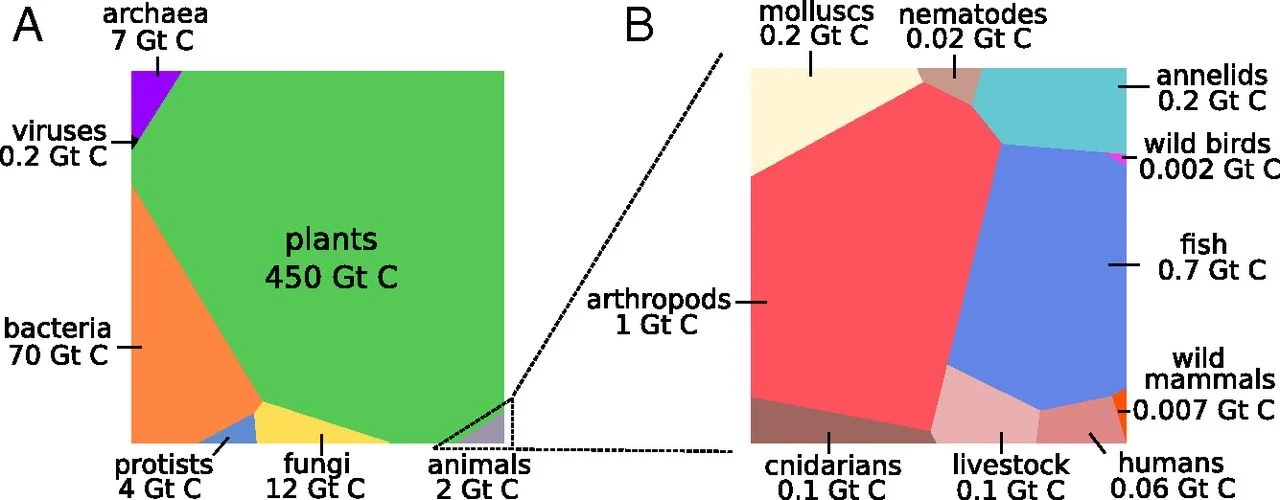
\includegraphics[width=1\linewidth]{./figs/pnas.1711842115fig01} 

}

\caption{Mass in giga tons of carbon for different groups of species. \citep{Bar-On2018}}\label{fig:carbonFixated}
\end{figure}

Note, that

\begin{itemize}
\item
  Plants are the most successful group in terms of the mass of carbon that they fixate.
\item
  Bacteria clearly dominate the more complex animal kingdom.
\item
  Animals represent a relative small fraction. Among animals, cattle and humans are over represented.
\end{itemize}

Other compelling evidence that there is no direction to evolution stems from the number of bacterial cells in our body. \citet{Sender2016} showed that the ratio of the number of bacterial cells to the number of human cells is close to 1. A human with a weight of 70kg has \(\pm\) 38 trillion bacterial cells and 30 trillion humane cells. Note, that trillion is a thousand billion or 10\(^{12}\)!

So, all these examples make clear that evolution has no direction. For every organism with a higher complexity there also emerge many organisms with lower complexity! However, we can view evolution as a creative process that is generating novel life forms that are well adapted to their environment.

\hypertarget{evolution-humanity-and-biodanza}{%
\section{Evolution, Humanity and Biodanza}\label{evolution-humanity-and-biodanza}}

First there was

\begin{enumerate}
\def\labelenumi{\arabic{enumi}.}
\item
  Chemical evolution: evolution of building blocks and chemistry of life.
\item
  Then, biological evolution of cells/organisms based on the selection of genetic information and function.
\item
  And finally, our species introduced cultural evolution that can bypass natural evolution using

  \begin{itemize}
  \tightlist
  \item
    artificial selection: breeding of plants, pets, cattle, genetic manipulation, etc.
  \item
    Technology: that enables us for a fast adaptation to new environments
  \end{itemize}
\end{enumerate}

Indeed, our upright walking life style gave our hands a new freedom that allowed homonids to make and use tools and weapons. This stimulated rapid brain development that eventually gave rise to the evolution of language and human consciousness, which is closely entwined with the evolution of technology and social relations \citep{capraLuisi2014}.

\hypertarget{consciousness}{%
\subsection{Consciousness}\label{consciousness}}

With this evolution a second type of consciousness arose, which is referred to as extended consciousness (see e.g. \citet{capraLuisi2014}). So on the one hand we have primary consciousness that is the cognitive process that is accompanied by basic perceptual, sensory and emotional experience, which gives an organism a sense of self here and now, and, is widespread among living organisms. On the other hand, extended consciousness involves a more elaborate self-awareness, an experience of identity, the ability for reflection and to hold mental images, which eventually enabled us to formulate values, beliefs, goals and strategies. From the evolution of language not only an inner world of concepts and ideas emerged but also a social world with organised relationships and culture \citep{capraLuisi2014}.

This organised social world has been key for our reproductive success. But, also came with profound consequences for our global ecosystem, which we changed in unprecedented ways. Our social organisation and human technology enabled us to make a giant jump from hominids who typically had a position in the middle of the food chain towards our position at the top of the food chain \citep{Harari2015}. Other species at the top of the food chain evolved over a course of millions of years into that position, which enabled ecosystems to slowly adapt to them. We, humans, however, took this spectacular leap so quickly that the ecosystem and our own psycho-emotional system had no time to adjust. Indeed, top predators are majestic creatures full of confidence as they evolved over millions of years with almost no natural enemies, while mankind took that position so quickly that we are still confronted with the fears and anxieties that are associated to species with a position at the middle of the food chain \citep{Harari2015}, which can have far reaching consequences on how we act and react.

Similar to biology, our social culture also evolves, but at a much faster and ever increasing pace.
Our current social culture, however, overemphasizes our extended consciousness, which led in extremis to the radical humanism of Decartes, which is summarized in his famous quote ``je pense donc je suis''.

Our self, however, is a mental image, which is very nicely worded by Brad Blanton in his book ``Radical Honesty'': ``We are the Being, the source of being and remembering. The creator of our own universe. We awaken in the womb into the ocean of experiences. Over a long period of time, that ocean becomes a sea of suggestions. We lose track of the ocean of experiences. We lose track of having created the sea. After we have lost track of everything sufficiently, we continue to interact with the sea and create a self. What we call the self is a creation of further interactions of the sea of suggestion. The being we were when we began, the being we actually still are, alive in an ocean of experience, including all the ocean as itself, recedes to the background of our attention, and the self we have created comes to the foreground. As we identify with our newly created self, we lose touch with the being we are and have been since light came on.'' \citep{Blanton1996}.

This has also been confirmed in scientific experiments. \citet{Kahneman2012}, for instance, showed in his cold water experiments that we have an experiencing self, which refers to our primary consciousness that resides in the ocean of experiences, and, a remembering or narrative self associated with our extended consciousness that can create mental images and memories of our experiences, which both play an important role in our decision making. In these experiments he exposed people to two treatments. In one treatment, a person's hand was immersed in cold water at 14 degrees for 1 minute. In the other treatment, he immersed their hand in water at 14 degrees for 1 minute, which is as annoying as the first treatment, and then the water temperature was raised to 15 degrees, which is only slightly less annoying, for an additional 30 seconds. Our experiencing self would never consider that extending the treatment with an episode of slightly warmer water makes the whole episode more appealing. But, when people were asked almost everyone preferred the longer treatment where the water is less cold at the end. Storing experiences happens according to a peak/end rule, i.e.~according to the maximum intensity of the experience and its ending, and, it is our remembering self that makes decisions. The peak/end rule is a heuristic that evolved biologically and allows us to quickly and efficiently store experiences without the burden to remember every instant of the entire episode. This rule works very well in general, however, it can lead to peculiar choices in specific situations.

\hypertarget{thinking-fast-and-slow}{%
\subsection{Thinking fast and slow}\label{thinking-fast-and-slow}}

In his book Thinking, Fast and Slow \citet{Kahneman2012} also discusses many other heuristics that lie at the heart of our decision-making. Indeed, he pointed out that we have two systems, a fast system and a slow system.

Fast thinking happens when facing problems that comes to mind automatically, e.g.~when seeing a picture of an angry person we immediately know that they is angry. This way of thinking happens through our instincts, emotions, intuition and associative activation. Experiences and words evoke memories, which evoke emotions that in turn trigger physiological responses, facial expressions and other reactions. This all happens extremely quickly and all at once and results in a self-reinforcing pattern of integrated cognitive, emotional, physiological and physical responses.

Slow thinking involves mental work and happens when we face problems for which the solution does not come to mind or that do not seem trivial. It is strongly associated with our extended consciousness. Note, however, that Kahneman points out that our slow thinking is also embodied. Indeed, during the slow thinking process our muscles tense up, our blood pressure rises, our heart rate increases and our pupils dilate, among others. Although many humans experience themselves as independent individuals who make their decisions in a rational and well thought out way, \citet{Kahneman2012} further argues that the majority of our decision making happens through fast thinking.

\hypertarget{implications-for-our-well-being-and-biodanza}{%
\subsection{Implications for our well-being and Biodanza}\label{implications-for-our-well-being-and-biodanza}}

It is thus important for our well-being to be well connected to our instincts and emotions. Indeed, as Rolando Toro pointed out, our instincts and emotions are the result of million of years of evolution. They are a cognition that has been shaped to maintain and reproduce our species, and are the result of the environments and evolutionary development that our ancestors, i.e.~humans and other species from which we evolved, underwent up to this point.

In our current society, however, there is a large emphasis on our extended consciousness. Moreover, information technology such as social media are also designed to hack our fast thinking process with the sole purpose to manipulate us for economic purposes. Together with the repression of our emotions and instincts this can invoke a dissociation between our cognitive processes, our bodily experiences and our needs, which in turn can lead to psycho-emotional pathologies. With Biodanza we strengthen our identity and with exercises evoking biological regression we feed our primary consciousness, which lets us reconnect with our perceptual, sensory and emotional experiences, and, our instincts, here and now. This can restore our primary cognition that has evolved over the course of millions of years. The vivencia can reactivate vital physiological and psycho-emotional processes and can have a deep impact on our being. Moreover, in the reactivation phase of the session, we reactivate our extended consciousness and often color our mental images and memories with the deep vivencial experience.

Now that we introduced how all species could evolve from their last universal common ancestor and touched upon some specific evolutionary aspects of our human species, we are ready to make the transition to how we humans evolve in our life span. This is also referred to as ontology, which is a another crucial biological aspect in the Model of Biodanza and is our focus in the next chapter.

\hypertarget{ontogenesis}{%
\chapter{Ontogenesis}\label{ontogenesis}}

In the middle of the model, we see the biological aspect ``ontogenesis'' indicated with the red box in Figure \ref{fig:modelOnto}, which is our focus in this chapter.

\begin{figure}

{\centering 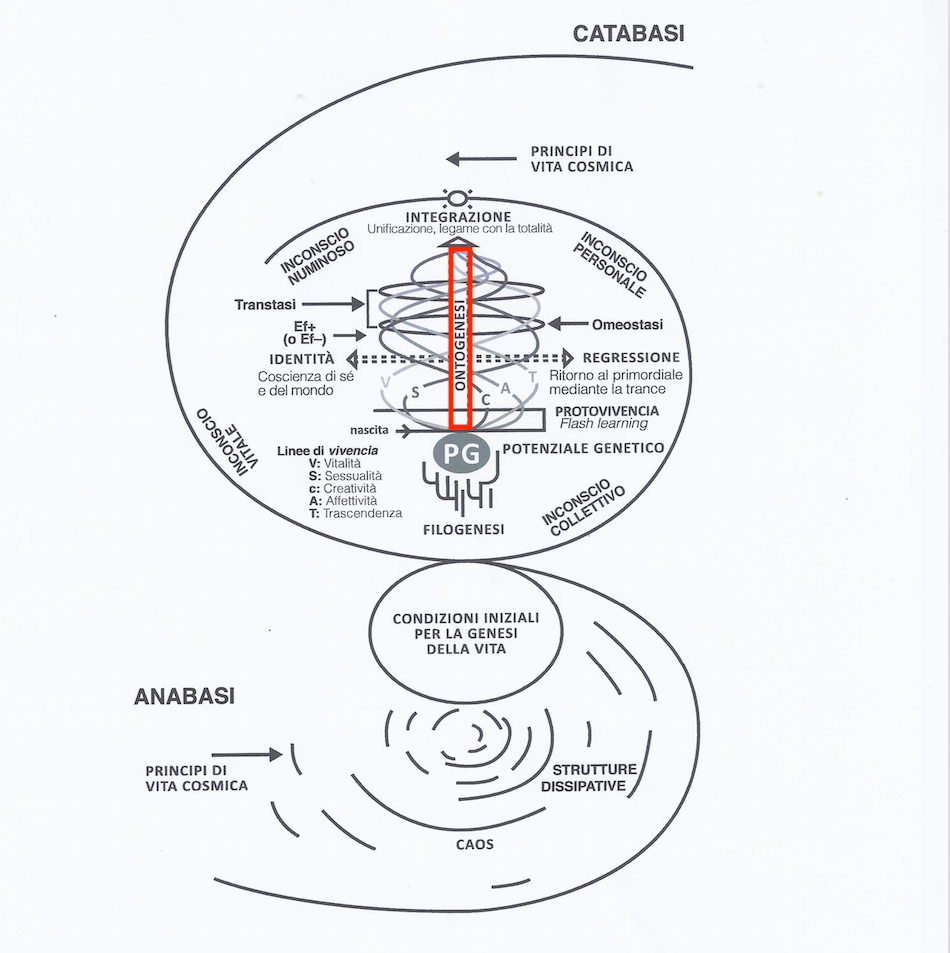
\includegraphics[width=0.5\linewidth]{./figs/biologischeAspectenBiodanzaDeelIII} 

}

\caption{Model of Biodanza and Ontogenesis}\label{fig:modelOnto}
\end{figure}

The ontogenesis is the development of an organism from a fertilized egg cell up to the adult stage until we eventually die.

Our ontogenesis starts from the genetic potential we inherit from our parents through their egg and sperm cell. The fertilized egg cell then starts to divide and at a certain point the cells start to differentiate into different tissues.
Each of our cells, apart from our germ cells, has the same genetic material!

Another very important factor in our development is our environment and how we interact with our environment.
Indeed, our phenotype, our observable traits and characteristics, stem from the complex interplay between our genomic makeup, our genotype, and environmental factors.

Key questions that arise in this respect is how cells of different tissues of the same organism that share the same genetic code can be morphologically so distinct, and how the environment and changes in our environment can impact our phenotype?

This is due to epigenetics! And, epigenetics is also the missing link that Rolando Toro needed to explain how Biodanza can provide an enriched environment that induces organic and cellular renewal, affective re-education and relearning of the original functions of life.

\hypertarget{epigenetics}{%
\section{Epigenetics}\label{epigenetics}}

Epigenetics is the study of how development, behavior and environment can cause changes that affect the way we use our genes. Unlike genetic changes, epigenetic changes are reversible and do not change your DNA sequence, but they can change how our body can (or cannot) read a DNA sequence, see Figure \ref{fig:epigenetics}.

\begin{figure}

{\centering \includegraphics[width=1\linewidth]{./figs/Epigenetic_mechanisms} 

}

\caption{Principes of epigenetics. Small molecules, epigenetic markers, interact with the DNA and histones. They can cause a gene to be accessible or inaccessible for RNA transcription (Source: NIH, Wikipedia)}\label{fig:epigenetics}
\end{figure}

Epigenetic markers, however, are copied during cell division to the two new cells that are formed. This causes a liver cell to remain a liver cell and a brain cell to remain a brain cell upon cell division.

Epigenetic markers are small molecules that interact either directly with the DNA or with histones, which are specific proteins that act as spools that wind the long DNA molecule in a more compact/condense form.
They can make genes accessible or inaccessible for RNA transcription and thus eventually for the production of proteins. Two common types are

\begin{itemize}
\tightlist
\item
  DNA methylation: binding a methyl group directly to DNA\footnote{A methyl group (-CH\(_3\)) consists of one carbon and three hydrogen atoms}.
\item
  Histone acetylation: binding an acetyl group to histone proteins\footnote{An acetyl group (-CO-CH\(_3\)) consists of two carbon, one oxygen and three hydrogen atoms}.
\end{itemize}

Both types can impact the activity of genes.
On the one hand DNA methylation actively represses the expression of a specific gene, while DNA demethylation enhances gene expression.
On the other hand histone acetylation makes the structure of a region of DNA more open and thus more accessible for transcription of the genes in that region, while de-acetylation has the opposite effect.

\hypertarget{epigenetics-during-embryonal-development}{%
\section{Epigenetics during Embryonal Development}\label{epigenetics-during-embryonal-development}}

Epigenetics plays an important role in embryonic development (see Figure \ref{fig:epiEmbryo}).



\begin{figure}

{\centering \includegraphics[width=1\linewidth]{./figs/DNA_methylation_reprogramming} 

}

\caption{Epigenetics in embryo genesis at CpG islands, regions that can bind with many methyl groups. All CpG islands of a sperm cell are almost fully methylated. That of an egg cell are methylated around 50\%. Upon fertilization the methylation drops and almost all genes become accessible for the undifferentiated blastula. As cells differentiate and get specific functions in tissues methylation increases again (Source: Mariuswalter, Wikipedia)}\label{fig:epiEmbryo}
\end{figure}

CpG islands are regions in our DNA that can be heavily methylated. They are major regulatory units and around 70\% of our genes have CpG islands in their promotor regions\footnote{A promoter is a sequence of DNA to which proteins bind to initiate transcription of the gene downstream of the promotor}. Methylation of the promotor region is typically associated with a reduction of gene expression. In Figure \ref{fig:epiEmbryo} we observe that the CpG islands of a sperm cell are almost fully methylated, which indicates that many genes are likely to be silenced. Indeed, a sperm cell has one main function and that is to swim forward and fertilize the egg cell. The CpG islands of an egg cell are methylated around 50\%. Upon fertilization the methylation drops in the blastocyst (an early stage of embryonic development, about five days upon fertilization). This is required for the cells to regain the property that they can divide and differentiate to all cell-types of the developing organism. As differentiation of the cells starts and as they evolve into tissues, methylation increases again so that the cells have access to less genes and get more specific functions. Note, that the methylation status is also passed upon cell division, which leads to invariance of differentiated cells: indeed, a liver cell remains a liver cell upon division and a brain cell a brain cell, etc.

\hypertarget{epigenetics-and-learning}{%
\section{Epigenetics and Learning}\label{epigenetics-and-learning}}

This section is largely based on the review article of Creighton et al.~entitled ``Epigenetic Mechanisms of Learning and Memory: Implications for Ageing'' \citep{Creighton2020}.

In the last decade, it has been shown that epigenetics is very important in development of the brain and for learning.

Animal research has shown that the disruption and inhibition of gene expression and translation in the brain shortly after a learning event has a tremendous impact on long time memories (\(\geq 24\) hours), but not on short term memories. These manipulation had most impact in the first hours upon the learning event. Suggesting that the initial memory consolidation happens within a 6 hour time window.

Learning typically happens in waves. Genes activated shortly after learning return to baseline within 24 hours, a time point at which a second wave of gene expression is triggered.
In the second wave genes are included that encode for epigenetic regulators.
So, the first wave within 6 hours upon learning is known to up regulate transcription factors important to initiate the second wave of transcription, which is needed to establish long-lasting memories.

\hypertarget{dna-methylation-and-memory}{%
\subsection{DNA Methylation and Memory}\label{dna-methylation-and-memory}}

In a large number of studies, DNA methylation has been shown to play an important role in multiple stages of memory formation.

On the one hand it is shown that DNA methylation is transient, i.e.~rapidly induced and reversed in the first hours upon learning. On the other hand, stably altered cortical DNA methylation has been shown up to 4 weeks upon learning and blocking the cortical DNA methylations has been shown to impair memory.
So methylation plays a role in different stages of the process of memory formation.

It also has been shown that methylation influences memory through different mechanisms, e.g.~

\begin{itemize}
\tightlist
\item
  Regulation of the activity of enhancers, i.e.~short DNA regions that enhance the transcription of genes
\item
  Alternative splicing, i.e.~transcribed RNA from a gene region is spliced by which certain exons, i.e.~coding stretches, are removed, resulting in the production of different gene products from the same gene. So methylation can change the specific gene products that are transcribed from a particular gene.
\item
  Expression of micro RNAs, short non-coding RNAs, that are biologically active.
\end{itemize}

A large body of literature support the role of methylation in learning and it is shown that methylation associated to learning occurs in the hippocampus, prefrontal cortex and the amygdala of the brain (Figure \ref{fig:brainRegionsLearning}).

\begin{figure}

{\centering \includegraphics[width=0.5\linewidth]{./figs/Brain_regions_in_memory_formation} 

}

\caption{Brain regions involved in memory formation. (Source: Wikipedia)}\label{fig:brainRegionsLearning}
\end{figure}

\hypertarget{histone-modifications-and-memory}{%
\subsection{Histone Modifications and Memory}\label{histone-modifications-and-memory}}

Another type of epigenetic regulation is through the modification of histones, i.e.~the proteins that act as spools around which the long DNA molecule is winded and which can affect the accessibility of a DNA region upon modification.

Histone modifications with epigenetic markers have been shown to be mainly important in the initial phase of memory consolidation. They are rapidly modified after which they return to baseline. These modifications cause ``winding or unwinding the DNA around or from the histones'' making particular genes accessible or inaccessible for expression.

Histone epigenetic markers seem to regulate the transcriptional sensitivity towards external stimuli. Histone acetylation that makes the DNA more accessible, for instance, has been shown to increase learning induced gene expression and seem to be particularly important for regulating memory strength.

So recent progress has shown the tremendous importance of epigenetics for brain development and learning, however, the field of neuro-epigenetics is still in its infancy and many open questions remain.

\hypertarget{epigenetics-and-aging}{%
\section{Epigenetics and Aging}\label{epigenetics-and-aging}}

Epigenetics are also largely driven by ecofactors. This can be nicely illustrated with identical twins who have almost the same genome\footnote{Identical twins have almost exactly the same genome, only very small differences have been build up in the womb}. It gets more easy to tell them apart over time due to epigenetic changes that are triggered by the different environments to which they were exposed and that effectively changed how they are using their genes. A good example is the difference in skin ageing between twins that had a different exposure to UV radiation (e.g.~Figure \ref{fig:epiUV}).



\begin{figure}

{\centering \includegraphics[width=0.5\linewidth]{./figs/dentical-twins-with-phenotypic-discordance-due-to-environmental-exposure-Although-MZ} 

}

\caption{Difference in skin ageing between twins is largely induced by epigenetic changes originating from a difference in exposure to UV radiation \citep{Schwab2017}}\label{fig:epiUV}
\end{figure}

Another twins study showed an association between physical exercise and epigenetic markers associated with a reduced development of metabolic syndrome \citep{Duncan2022}. Indeed, by studying monozygotic twins with one person that was physical more active than the other member of the twin, the researchers minimized the genetic differences between active and inactive participants in the study. This setup allowed them to discover regions that were differentially methylated between active and inactive participants, while controlling for their genetic make-up. The methylation alterations that were found were associated with genes that are known to be involved with physical activity and obesity.

Aging and longevity are influenced by genetic, epigenetic, and environmental factors during development, growth, maturity, and older stages.
It has been shown that the genetic component (heritability) plays only a moderate role in aging and longevity, so epigenetics seems to be a major contributor \citep{Adwan2018}. Indeed, many epigenetics markers and in particularly DNA methylation sites have been shown to be remarkable predictors of chronological age.
Aging has been shown to be associated
with profound changes in the epigenetic landscape, that give rise to alterations of gene expression and genome architecture.

An important modes of action in ageing has been shown to be through the association of epigenetics and telomere length.

Telomeres are regions of repetitive nucleotide sequences associated with specialized proteins at the ends of our chromosomes, see Figure \ref{fig:telomeres}. Each cell division the telomeres get shorter and the telomere shortening has been associated with ageing of cells, tissues and organs.

\begin{figure}

{\centering \includegraphics[width=0.8\linewidth]{./figs/telomeres} 

}

\caption{Telomeres are repetitive nucleotide sequences at the end of a chromosome. Each time a cell divides the telomeres on the end of the chromosome get smaller. The average cell will divide between 50 and 70 times before cell death (Source: Wikipedia).}\label{fig:telomeres}
\end{figure}

\citet{BlackburnEpel2017} use the plastic ends of shoelaces as an analogy for telomeres. If these ends shorten, the shoelace is prone to start fraying. Indeed, if the telomeres are getting too short, the integrity of the chromosome is at risk in the next cell division. Therefore a cell with too short telomeres goes into senescence: it stops with cell division, which will eventually lead to cell death.

However, through an enzyme complex called telomerase, the telomeres can be extended. So in the shoe lace analogy telomerase is the glue with which we could restore the plastic caps of a shoelace.

There is growing evidence that telomeres play a role in age-related processes. Indeed, mutations in telomerase and telomere genes causing increased telomere shortening, occur in patients with age-related disease, such as degenerative organ failure and a cancer-prone state among others. Moreover, causal links between telomere loss, cellular senescence (increasing cell death rates) and aging have been established with genetically modified animal models \citep{Adwan2018}.

Epigenetics has also been shown to play an important role in telomere maintenance \citep{Adwan2018}.
Multiple studies showed that telomeric and subtelomeric regions contain histone modifications and subtelomeric DNA can undergo methylation.
Here, the epigenetic modification does not induce changes in the expression of target genes but affects telomere length or telomere structure.
Moreover, genes involved in the production of telomerase also have been shown to be under the regulation of methylation.

\hypertarget{epigenetics-and-stress}{%
\section{Epigenetics and Stress}\label{epigenetics-and-stress}}

Epigenetics also have been shown to be a key mechanism by which stressors interact with the genome.
This leads to stable changes in DNA structure, gene expression, and behavior (e.g. \citet{Park2019}).

Interestingly, stress and depression are mainly
associated with epigenetic alterations in genes involved in mediating resilience, vulnerability to stress, and stress-response related genes (e.g. \citet{Park2019}).

In their book ``the telomere effect'' \citet{BlackburnEpel2017} give an overview of their studies on the impact of stress on telomere length and telomerase activity.
They introduce many compelling examples and study results that underpin that ageing effects are strongly impacted by stress during childhood as well as by long-lasting stress on later age. And this, through the mediation of telomerase activity and telomere length, which we argued to be largely under control of epigenetics in the previous section.

\citet{BlackburnEpel2017} also discuss studies where it was shown that mind-body techniques such as meditation, qigong and yoga, among others are stress reducing, have positive effects on our well-being, can prevent inflammation and can induce cell rejuvenation by (re-)activating the gene that is encoding for teleomerase, among others. These effects were observed in well designed experiments and are in line with the beneficial effects that Rolando Toro also envisioned to induce through his System of Biodanza.

\hypertarget{ontogenesis-in-the-model-biodanza}{%
\section{Ontogenesis in the Model Biodanza}\label{ontogenesis-in-the-model-biodanza}}

So epigenetics represents the scientific explanation for Ontogenesis in the Rolando Toro's System of Biodanza. Indeed, with a quote of Rolando ``Es que en la epigénesis
se permite o no la expresión de los genes existentes'' \citep{Montanari2023}. So, it is through epigenetics that the expression of existing genes is allowed or not.

Hence, our ontogenesis, the formation of our phenotype, does not directly stem from our genome, but is the result of the modulation mechanism on our genome, i.e.~the activation and inhibition of the expression of our genes we inherited from our parents.

Rolando further argued that ``We have many genes that are not good (\ldots) It is epigenetics, through the enriched environment, that prevents or allows the expression of some aspects of the genetic code (\ldots) Sometimes the environment does not block the malignant genes, then the pathology appears'' \citep{Montanari2023}. With this respect practicing Biodanza can be seen as a regular administration of stimuli through vivencia that trigger changes and repairs necessary to rebalance our biological system from the damage caused by our toxic experiences and the attacks of pathogenic agents \citep{Montanari2023}.

In this chapter we introduced the biological angle of ontogenesis with which we conclude the biological aspects of the Model of Biodanza. Here, we focused exclusively on the pure biological component of ontogenesis. Note, however, that it is not our intention to reduce ontogenesis in the model of Biodanza to these biological aspects, only. Indeed, the biological development of an individual takes place in a larger field as it also involves an important social, psychological and emotional component because an important part of human life takes place in the symbolic social domain.

This larger and important intersection of the life sciences, physiology, anthropology, sociology, psychology, art and mysticism is well beyond the scope of this monograph. It is in this larger field that Rolando was operating when he developed his system of Biodanza. So these aspects are also key for understanding growth and integration of an individual towards a state which Rolando referred to with his metaphor ``the cosmic human''.

\hypertarget{concluding-remarks}{%
\chapter{Concluding Remarks}\label{concluding-remarks}}

My writing was my humble attempt to convey my passion for the system of Biodanza and vibrating it to you. I hope that I was able to bring the message across

\begin{itemize}
\item
  That life is deeply rooted in the universe
\item
  That life is one
\item
  That life is an emergent property that arises on different levels: from the chemical level, over cellular, tissue, organ, organ system, organism, community, ecosystem level upto the level of our entire planet, and that this also involves our human life that largely takes place in the symbolic social domain.
\item
  That life is a gestalt of environment, cognition and an autopoietic unit (i.e.~a cell, or organism, or ecosystem, \ldots), which can be viewed as an embodied mind.
\item
  How each of these levels and thus also our psycho-socio-emotional realm share the same ``bio-logic'' or pattern of organisation, which invites us to deeply respect and to learn from all forms of life around us.
\end{itemize}

These insights makes a biocentric world view very natural, which was Rolando's starting point when he developed his system of Biodanza. With Biodanza he envisioned to create an enriched environment with regular administration of stimuli through vivencia that can rebalance our biological system and can have a large impact on our ontogenesis.

Indeed, vivencia has a strong impact on our body and brain. The sensations that we experience have a physiological impact through the modulation of our genes that encode for a diverse scala of proteins, hormones and neurotransmitters.

Vivencia also have the quality that they immediately access our embodied mind through experience that precedes our extended consciousness. So it enables us to learn by strong experiences that directly tap into our personal, collective and vital unconsciousness.

These transformative experiences through vivencia can be imprinted by epigenetics, which can induce important changes at a physiological level and also is a driver for mechanisms of learning and memory.

Indeed, as Biodanza practitioners we are familiar with the long lasting memories to deep vivencia, and with how practicing Biodanza also induces change.
Change in how we feel, stand in life, interact socially and with our environment.

I also hope that this monograph will trigger you to continue on your Biodanza path with even more enthusiasm. Indeed, it is a unique path to promote your ontogenesis and well-being, and it invites you to reconnect with yourself, the others, and the entire world surrounding you. Moreover, it might also change the larger autopoietic social system in which you are embedded. And this, as Rolando Toro envisioned, by effectively switching it to another attractor through its positive feedback on your change, growth and interaction.

\hypertarget{addendum}{%
\chapter*{Addendum}\label{addendum}}
\addcontentsline{toc}{chapter}{Addendum}

Below you will find some additional texts and impressions that I have written during my Biodanza teacher training.

\hypertarget{reflection-on-my-first-biodanza-retreat-with-annette-heynderickx-in-buirefontaine}{%
\section*{Reflection on my first Biodanza retreat with Annette Heynderickx in Buirefontaine}\label{reflection-on-my-first-biodanza-retreat-with-annette-heynderickx-in-buirefontaine}}
\addcontentsline{toc}{section}{Reflection on my first Biodanza retreat with Annette Heynderickx in Buirefontaine}

Heel onverwachts en op de valreep verschenen we met zijn twee op Buirefontaine.\\
En dat was alsof het zo moest zijn.

Al meteen in de eerste sessie kregen we de kans om elkaar als koppel het mooiste cadeau te schenken:\\
Onszelf,\\
in zachtheid aangekomen,\\
en in alle veiligheid opgenomen in een nieuwe groep,\\
waardoor we elkaar volledig geopend en in volle afstemming\\
opnieuw echt mochten ontmoeten.

Een diepe intense ontmoeting,\\
waarin we een hectisch jaar van zorg af mochten sluiten.\\
Iets wat ons mentaal al langer duidelijk was,\\
maar wat we op een of andere manier nog niet samen konden doorvoelen.

En die ontmoeting liet dat in al zijn eenvoud en echtheid transformeren.\\
Het was voor ons de kern van onze eerste vivencia (beleving),\\
en tegelijk het begin van een intense reis die voor ons verscholen lag in het anagram die jij, Annette, legde.

Tijdens volgende vivencia's konden we in ``de dans van de donder'' de kracht ervaren in onszelf en die ook zien in de ander;\\
om dan het mannelijke en vrouwelijke dat in ieder van ons schuilt te verkennen en te vieren;\\
waarna de dans van de chaos ons uitnodigde om connectie te maken met het donkere in onszelf,\\
dat donkere waar we zelf vaak blind voor zijn,\\
en waar ook die scheppende kracht in verscholen ligt om als een kiem door te breken naar het nieuwe licht.

En als je te midden van een vivencia even dreigde te overspoelen of te vervloeien,\\
was er steeds die zorg, van jou, van jullie en van de volledige groep,\\
zodat je die emotie, die beleving, die vivencia telkens opnieuw kon gaan containen.\\
En dat gebeurde in alle eenvoud door een zorgende blik, een ontmoeting, een omhelsing, \ldots{}

Dat is net de kracht van Biodanza,\\
het nodigt je zo uit om te voelen, om af te stemmen en om te connecteren op een dieper weten waardoor je gaat transformeren.\\
Het laat je versmelten met alle polen in jezelf,\\
met je partner,\\
met ieder uit de groep,\\
en met ``de elementen van het leven'' die we dansten,\\
waardoor je echt gaat ervaren,\\
waardoor het denken voelen wordt,\\
en daarna een innerlijk diep weten.

En dat is een kunst die jij, Annette, als geen ander verstaat en weet over te brengen.\\
Je lichaam spreekt,\\
je dans nodigt uit om te beleven,\\
jij en Frank scheppen de bedding van de groep met zoveel kracht,\\
zodat ieder zichzelf en de ander mag en kan ervaren,\\
zonder oordeel en zonder te veel woorden.

De reis was heel inspirerend,\\
het anagram werkt door \ldots{}

Fien \& Lieven - Juli 2020

\hypertarget{poetic-impressions-of-some-vivencia}{%
\section*{Poetic impressions of some vivencia}\label{poetic-impressions-of-some-vivencia}}
\addcontentsline{toc}{section}{Poetic impressions of some vivencia}

\hypertarget{de-fysiologische-loop}{%
\subsection*{De fysiologische loop}\label{de-fysiologische-loop}}
\addcontentsline{toc}{subsection}{De fysiologische loop}

Mijn bewustzijn zakt\\
van mijn hoofd\\
in mijn lichaam.\\
Ik voel en neem waar.\\
Spanning wordt ontspanning.\\
Ik laat los\\
en beweeg.\\
Het doen\\
wordt langzaam\\
zijn.

\hypertarget{ritmische-couxf6rdinatie}{%
\subsection*{Ritmische coördinatie}\label{ritmische-couxf6rdinatie}}
\addcontentsline{toc}{subsection}{Ritmische coördinatie}

Met mijn hand voel ik de ander\\
en we worden samen één.\\
Eén in de beweging,\\
één met de beweging.\\
Ik kleur jou\\
en jij kleurt mij.\\
We kleuren samen.\\
En na de wissels\\
regenbogen.

\hypertarget{lopen-met-vastberadenheid}{%
\subsection*{Lopen met vastberadenheid}\label{lopen-met-vastberadenheid}}
\addcontentsline{toc}{subsection}{Lopen met vastberadenheid}

Ik voel de muziek\\
en wordt geladen.\\
Ik stuur mezelf naar voor,\\
naar die overkant.\\
En dan terug.

Langzaam laat ik los.\\
En bij de derde oversteek,\\
wandel ik gewoon.\\
Vastberaden en toch ontspannen.

Ik voel die kracht en groei.\\
Ik groei in grootsheid\\
vanuit ontspanning.\\
En dat Groot-Zijn\\
zindert na.

\hypertarget{de-ontmoeting}{%
\subsection*{De ontmoeting}\label{de-ontmoeting}}
\addcontentsline{toc}{subsection}{De ontmoeting}

Vanuit dat Groot-Zijn\\
zie ik jou.\\
Ik zie jouw Groot-Zijn\\
en jij die van mij.

Stap voor stap\\
kom je bij mij binnen\\
en ik bij jou.

Onze aura's gaan versmelten\\
en onze handen raken aan.\\
Onze ogen vinden de weg\\
heel diep bij elkaar naar binnen.\\
Daar alwaar die puurheid\\
in ons schuilt.

Diep geraakt\\
gaan we in omhelzing\\
en we voelen na.

\hypertarget{fluuxefditeit-in-compacte-groep}{%
\subsection*{Fluïditeit in compacte groep}\label{fluuxefditeit-in-compacte-groep}}
\addcontentsline{toc}{subsection}{Fluïditeit in compacte groep}

Ik voel en beweeg.\\
Ik ontmoet\\
en ga verder.\\
Ik raak aan\\
en word aangeraakt.\\
Steeds opnieuw\\
en als maar verder.

We bewegen en voelen\\
we omhelzen en woelen\\
samen zijn we één.

We vloeien samen\\
helemaal terug\\
naar de oceaan.\\
Intens aangekomen\\
in onze oorsprong\\
zijn we één.

Muziek wordt zachter \ldots{}\\
Van oceaan terug naar druppels.\\
Vanuit het één worden we twee.\\
En dan weer één.

Je groeit uit mij\\
in al je puurheid,\\
daar zomaar in mijn oksel.\\
En ik groei uit jou.\\
Uit je armen en je handen,\\
diep en zacht,\\
en zo intens.

Langzaam wiegend\\
open ik mijn ogen en\\
zie ik wie je bent.\\
Langzaam wiegend\\
open ik mijn ogen en\\
zie ik wie ik ben.

Daarna allen samen\\
zo open en zo zacht\\
In die intense cirkel\\
schrijven we elk\\
die nieuwe herinnering

Een herinnering\\
sterk en diep\\
en o zo transformerend.\\
De weg naar de oceaan\\
is voor mij opnieuw geopend.

De weg die wacht\\
en roept\\
van zodra muziek\\
en dans weerklinkt.

\hypertarget{minotaurus}{%
\subsection*{Minotaurus}\label{minotaurus}}
\addcontentsline{toc}{subsection}{Minotaurus}

Jij Minotaurus,\\
Toont ons het menszijn in al haar facetten.

In het epicentrum van het veld van de aanwezige cirkel worden we herboren.\\
Een zachte welp wordt een krachtige tijger.\\
Een beer danst zijn angsten voor wilde dieren.\\
Drenkelingen geven zich over en durven zich kopje onder te laten gaan om daarna het vertrouwen te vinden om zich te laten redden en het leven te omarmen.

En ten midden van dit alles breng je voor mij de kracht van het loslaten,\\
van niet te redden voor er wordt uitgereikt.\\
De kracht van samen\\
te zakken naar een eindeloze diepte\\
En om daar dan te blijven staan \ldots{}

Daar beneden\\
word ik jij\\
En jij wordt ik\\
Omarmd dragen we elkaar\\
terug naar de oppervlakte.\\
Met jou Minotaurus\\
als ons baken,\\
een baken van liefde.

\hypertarget{how-quantum-mechanics-turned-the-cartesian-scientific-world-view-upside-down}{%
\section*{How quantum mechanics turned the Cartesian scientific world view upside down}\label{how-quantum-mechanics-turned-the-cartesian-scientific-world-view-upside-down}}
\addcontentsline{toc}{section}{How quantum mechanics turned the Cartesian scientific world view upside down}

Quantum mechanics invites us to let go the old Cartesian way of causal thinking.

In the Cartesian paradigm most processes are considered to be continuous and as soon as the initial conditions, such as position and velocity of particles, are known all future conditions can be derived from it. This led to our traditional deterministic world view and our associated cause and effect mind set.

In quantum mechanics, however, energy can only be transferred in indivisible units, quanta, and we only know the probability that a quantum of energy will be transferred. Moreover, we do not now exactly when and where it will be transferred. The same holds for position and momentum\footnote{Mass \(\times\) Velocity} of matter. Particularly, probabilities for the possible results of measurements can be derived from the wave function that is used in quantum mechanics to represent matter. The theory further implies that both light and matter will display wave-like or particle-like characteristics depending on their interaction with its environment, which has been validated in many experiments. Moreover, also long range correlations have been shown to exist between so-called ``entangled particles'' that were separated by a large distance\footnote{Quantum entanglement occurs when a group of ``particles'' are generated or interacted in a way such that the quantum state of each ``particle'' of the group cannot be described independently of the state of the others, even when the ``particles'' are subsequently separated by a large distance.}. So our world view can no longer remain deterministic, but, rather has to becomes probabilistic in nature.

The quantum characteristics are especially observable on a microscopic level. On a macroscopic scale, however, processes typically involve so many quanta and/or an aggregate of so many ``particles'' that we can reason on the average energy and/or average position and momentum at this scale. This, however, can be predicted in very narrow limits because we average over so many quanta or particles. Interestingly, the classical deterministic laws provide a good approximation for the average energy transfer and/or position and momentum of large matter aggregates. Moreover, a quantum is also a very tiny unit of energy so at a macroscopic scale the observed energy transfer involving many quanta also appears to be almost continuous.

This clearly shows that scientific theories are ever-changing insights that are giving shape and form to how we view and experience the world; and more importantly that we have to remain open to change our mind set.

  \bibliography{bibliography.bib}

\end{document}
